\documentclass[aspectratio=169]{beamer}

\usepackage{graphicx}
\usepackage{amsmath,amssymb}
\usepackage{ragged2e}
\usepackage{tikz}
\usepackage{xcolor}
\usepackage{array}

\usetikzlibrary{arrows.meta,positioning}

\graphicspath{{./}{../MACC2026/Figures/}{../report/figures/2026-04-30_lyapunov_results_synthesis/}}

\definecolor{maroon1}{rgb}{0.478, 0, 0.235}
\definecolor{lightgray}{rgb}{0.94,0.94,0.97}
\definecolor{lightgray2}{rgb}{0.5,0.5,0.5}
\definecolor{maccblue}{RGB}{28,74,117}
\definecolor{maccgreen}{RGB}{44,118,92}
\definecolor{maccred}{RGB}{156,58,52}

\usetheme{Copenhagen}
\usecolortheme[named=maroon1]{structure}

\setbeamerfont{caption}{size=\scriptsize}
\setbeamertemplate{navigation symbols}{}
\setbeamercolor{block body}{fg=black,bg=lightgray}
\setbeamercolor{block title}{fg=white,bg=maroon1}

\newcommand{\refnote}[1]{{\bfseries\color{maroon1}\scriptsize (#1)}}
\newcommand{\takeaway}[1]{%
\vspace{0.04cm}
{\scriptsize\color{maroon1}\textbf{Takeaway:} #1}
}

\setbeamercolor{takeawaybox}{fg=black,bg=maroon1!8}

\newcommand{\takeawaybox}[1]{%
\vspace{0.01cm}
\begin{center}
\begin{beamercolorbox}[wd=0.94\textwidth,sep=3pt,center,rounded=true,shadow=false]{takeawaybox}
\scriptsize
\textbf{\textcolor{maroon1}{Takeaway:}} #1
\end{beamercolorbox}
\end{center}
}

\setbeamercolor{pone title}{fg=white,bg=maccblue}
\setbeamercolor{pone body}{fg=black,bg=maccblue!8}
\setbeamercolor{ptwo title}{fg=white,bg=maccgreen}
\setbeamercolor{ptwo body}{fg=black,bg=maccgreen!8}
\setbeamercolor{pthree title}{fg=white,bg=maccred}
\setbeamercolor{pthree body}{fg=black,bg=maccred!8}

\expandafter\def\expandafter\insertshorttitle\expandafter{%
\insertshorttitle\hfill%
\insertframenumber\,/\,\inserttotalframenumber}

\title[Stats and Control 2026]{%
\textbf{A Practical Reinforcement Learning Control Framework\\
for Complex Process Systems}}

\author[A. H. Hamedi]{%
A. H. Hamedi\\[-0.2ex]
{\scriptsize Supervisor: P. Mhaskar}}

\date[Stats and Control 2026]{%
{\scriptsize Stats and Control 2026}\\[-0.1ex]
{\scriptsize Kingston University}}

\begin{document}

%============================= Slide 1 ============================
\begin{frame}
\setbeamertemplate{blocks}[rounded][shadow=false]
\setbeamercolor{block body}{fg=white,bg=maroon1}

\vspace{0.15cm}

\begin{center}

\includegraphics[width=.7\textwidth, height=0.25\linewidth]{figures/logo.png}
\end{center}

\vspace{0.25cm}

\begin{block}{}
\begin{center}
\parbox{0.92\textwidth}{\centering
\Large \textbf{A Practical Reinforcement Learning Control Framework\\
for Complex Process Systems}}
\end{center}
\end{block}

% \vspace{0.30cm}

\begin{center}
{\large \textbf{A. H. Hamedi}}\\[0.25ex]
{\scriptsize Supervisor: P. Mhaskar}\\[1.0ex]

{\scriptsize \color{maroon1} Department of Chemical Engineering, McMaster University}\\[0.45ex]
{\scriptsize \color{lightgray2} In collaboration with Linde plc.}\\[0.8ex]

% {\scriptsize \color{lightgray2} Stats and Control 2026}\\[-0.1ex]
\vspace{-0.25cm}
{\scriptsize \color{lightgray2} Kingston University}
\end{center}

\end{frame}

%============================= Slide 2 ============================
\begin{frame}
\setbeamertemplate{blocks}[default]
\setbeamercolor{block body}{fg=black,bg=lightgray}
\frametitle{\large \textbf{Outline}}
\small

\begin{block}{Central question}
\justifying
How can reinforcement learning improve constrained chemical process control while keeping the controller practical, interpretable, and safe?
\end{block}

\vspace{0.08cm}

\begin{enumerate}\justifying
  \setlength\itemsep{0.35ex}

  \item Motivation: why fixed linear MPC and naive online RL each face practical limits

  \item Problem settings: the polymer reactor benchmark and the Aspen Dynamics \(C_2\) splitter

  \item \textbf{Project 1} \textcolor{maccblue}{(published)}: MPC-pretrained RL with offset-aware online adaptation

  \item \textbf{Project 2} \textcolor{maccgreen}{(ongoing)}: RL-assisted MPC as a supervisory adaptive layer

  \item \textbf{Project 3} \textcolor{maccred}{(ongoing)}: direct Lyapunov target MPC and pretrained-RL safety gate

  \item \textbf{Closing:} Main takeaways, current limitations, and next steps

\end{enumerate}

\end{frame}

%============================= Slide 3 ============================
\begin{frame}
\setbeamertemplate{blocks}[default]
\setbeamercolor{block body}{fg=black,bg=lightgray}
\frametitle{\large \textbf{MPC works through its model, and the model is the bottleneck}}
\scriptsize

\vspace{-0.28cm}

\begin{columns}[T,onlytextwidth]

\begin{column}{0.56\textwidth}

\begin{block}{Why MPC is the right baseline}
\begin{itemize}\justifying
  \setlength\itemsep{0.35ex}

  \item MPC uses an internal process model to predict future behavior and optimize inputs under constraints
  {\bf \color{maroon1} \scriptsize (Rawlings et al., 2017)}.

  \item That model lets MPC coordinate multivariable decisions online.
\end{itemize}
\end{block}

\vspace{0.02cm}

\begin{block}{Why the model becomes the bottleneck}
\begin{itemize}\justifying
  \setlength\itemsep{0.35ex}

  \item \textbf{First-principles models:} mechanistic, but expensive to build and hard to maintain for large changing plants
  {\bf \color{maroon1} \scriptsize (Daoutidis et al., 2023)}.

  \item \textbf{Data-driven models:} flexible, but they need informative data, monitoring, and revalidation
  {\bf \color{maroon1} \scriptsize (Hassanpour et al., 2020)}.
\end{itemize}
\end{block}

\end{column}

\begin{column}{0.41\textwidth}
\centering

\vspace{0.5cm}

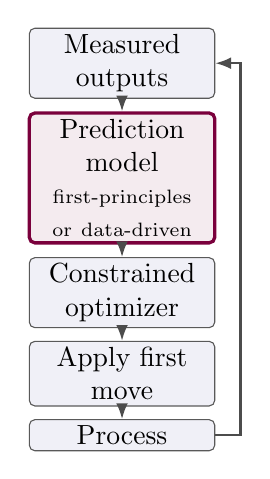
\begin{tikzpicture}[
  node distance=0.16cm,
  box/.style={draw=black!65, rounded corners=2pt, align=center,
  fill=lightgray, inner sep=2.2pt, text width=2.20cm},
  keybox/.style={draw=maroon1, very thick, rounded corners=2pt,
  align=center, fill=maroon1!8, inner sep=2.2pt, text width=2.20cm},
  arrow/.style={-{Latex[length=2.0mm]}, thick, draw=black!70}
]
\node[box] (measure) {Measured\\outputs};
\node[keybox, below=of measure] (model) {Prediction model\\[-0.1ex]\scriptsize first-principles or data-driven};
\node[box, below=of model] (opt) {Constrained\\optimizer};
\node[box, below=of opt] (move) {Apply first\\move};
\node[box, below=of move] (plant) {Process};

\draw[arrow] (measure) -- (model);
\draw[arrow] (model) -- (opt);
\draw[arrow] (opt) -- (move);
\draw[arrow] (move) -- (plant);
\draw[arrow] (plant.east) -| ++(0.32,0) |- (measure.east);
\end{tikzpicture}

\vspace{0.06cm}

{\tiny \textbf{Figure:} MPC relies on a prediction model inside the closed loop, so controller quality tracks model quality.}

\end{column}

\end{columns}

\takeawaybox{MPC performance depends directly on model quality and model upkeep.}

\end{frame}

%============================= Slide 4 ============================
\begin{frame}
\setbeamertemplate{blocks}[default]
\setbeamercolor{block body}{fg=black,bg=lightgray}
\frametitle{\large \textbf{Industry uses linear MPC because it is practical, but validity is local}}
\scriptsize

\vspace{-0.28cm}

\begin{columns}[T,onlytextwidth]
\begin{column}{0.56\textwidth}

\begin{block}{Why linear MPC remains common}
\begin{itemize}\justifying
  \setlength\itemsep{0.35ex}

  \item Linear MPC remains a practical industrial choice for constrained multivariable process control
  {\bf \color{maroon1} \scriptsize (Darby et al., 2012)}.

  \item Linear empirical models are easier to identify, validate, and maintain than large nonlinear models.

  \item The resulting online optimization problem is tractable and well understood.
\end{itemize}
\end{block}

\vspace{0.02cm}

\begin{block}{Why linear MPC still faces problems}
\begin{itemize}\justifying
  \setlength\itemsep{0.35ex}

  \item One linear model is usually most accurate near the operating region where it was identified.

  \item Nonlinearity, plant drift, and disturbances can create prediction error, offset, and retuning needs.
\end{itemize}
\end{block}

\end{column}

\begin{column}{0.41\textwidth}
\vspace{0.5cm}
\centering
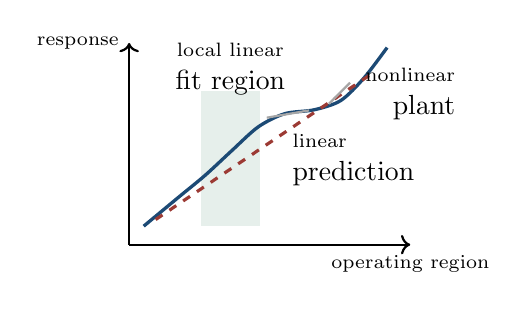
\begin{tikzpicture}[x=0.84cm,y=0.84cm]
  \fill[maccgreen!12] (1.08,0.28) rectangle (1.98,2.32);
  \draw[->,thick] (0,0) -- (4.25,0) node[below] {\scriptsize operating region};
  \draw[->,thick] (0,0) -- (0,3.05) node[left] {\scriptsize response};

  \draw[line width=1.2pt,maccblue]
    plot[smooth] coordinates {(0.22,0.28) (0.75,0.72) (1.15,1.05) (1.55,1.42) (1.95,1.78) (2.35,1.98) (2.8,2.04) (3.2,2.18) (3.55,2.52) (3.9,2.98)};

  \draw[line width=1.15pt,dashed,maccred] (0.4,0.38) -- (3.72,2.62);

  \node[align=center] at (1.53,2.66) {\scriptsize local linear\\fit region};
  \node[align=right] at (4.25,2.28) {\scriptsize nonlinear\\plant};
  \node[align=left] at (3.39,1.28) {\scriptsize linear\\prediction};

  \draw[thick,gray!70] (2.08,1.92) -- (2.72,2.03);
  \draw[thick,gray!70] (3.02,2.13) -- (3.34,2.45);
\end{tikzpicture}

\vspace{0.06cm}

{\tiny \textbf{Figure:} a linear model can match well near its identification region, then diverge as the plant moves away from nominal operation.}

\end{column}
\end{columns}

\takeawaybox{Linear MPC is practical and useful, but it becomes a local controller when plant behavior moves outside the identification region.}

\end{frame}

%============================= Slide 5 ============================
\begin{frame}
\setbeamertemplate{blocks}[default]
\setbeamercolor{block body}{fg=black,bg=lightgray}
\frametitle{\large \textbf{RL learns a policy from interaction and long-horizon reward}}
\scriptsize

\vspace{-0.30cm}

\begin{columns}[T,onlytextwidth]

\begin{column}{0.40\textwidth}
\centering
\vspace{1cm}

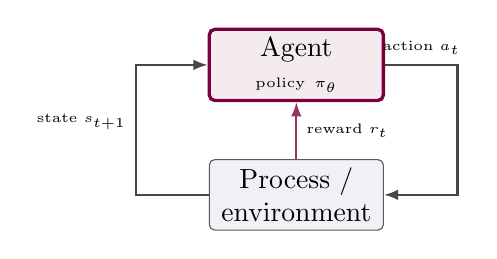
\begin{tikzpicture}[
  box/.style={draw=black!65, rounded corners=2pt, align=center,
  fill=lightgray, inner sep=3pt, text width=2.00cm, minimum height=0.58cm},
  keybox/.style={draw=maroon1, very thick, rounded corners=2pt, align=center,
  fill=maroon1!8, inner sep=3pt, text width=2.00cm, minimum height=0.58cm},
  arrow/.style={-{Latex[length=1.8mm]}, thick, draw=black!72},
  rarrow/.style={-{Latex[length=1.8mm]}, thick, draw=maroon1!80}
]
\node[keybox] (agent) at (0,1.20) {Agent\\[-0.2ex]\tiny policy \(\pi_\theta\)};
\node[box] (env) at (0,-0.45) {Process /\\environment};

\draw[arrow] (agent.east) -- node[above] {\tiny action \(a_t\)} ++(0.92,0) |- (env.east);
\draw[arrow] (env.west) -- ++(-0.92,0) |- node[pos=0.28,left] {\tiny state \(s_{t+1}\)} (agent.west);
\draw[rarrow] (env.north) -- node[right] {\tiny reward \(r_t\)} (agent.south);
\end{tikzpicture}

\vspace{0.05cm}

{\tiny \textbf{Figure:} RL updates a policy from interaction data and long-horizon reward.}

\end{column}

\begin{column}{0.58\textwidth}

\begin{block}{What the controller learns}
\justifying
The agent maps state to action, \(a_t=\pi_\theta(s_t)\), and learns from transition data \((s_t,a_t,r_t,s_{t+1})\). The policy is improved by increasing
\[
J(\theta)=\mathbb{E}_{\pi_\theta}\!\left[\sum_{k=0}^{\infty}\gamma^k r_{t+k}\right].
\]
\end{block}

\vspace{0.02cm}

\begin{block}{Why this is attractive for control}
\begin{itemize}\justifying
  \setlength\itemsep{0.25ex}
  \item Once trained, the policy can provide fast nonlinear feedback.
  \item RL is attractive for nonlinear or time-varying plants, but the training data and reward design become critical
  {\bf \color{maroon1} \scriptsize (Nian et al., 2020)}.
\end{itemize}
\end{block}

\end{column}
\end{columns}

\vspace{-0.03cm}
\takeawaybox{RL can learn long-horizon feedback, but process-control RL still needs carefully designed data and rewards.}

\end{frame}

%============================= Slide 6 ============================
\begin{frame}
\setbeamertemplate{blocks}[default]
\setbeamercolor{block body}{fg=black,bg=lightgray}
\frametitle{\large \textbf{Those RL assumptions break in industrial process control}}
\scriptsize

\vspace{-0.28cm}

\begin{columns}[T,onlytextwidth]

\begin{column}{0.43\textwidth}
\centering
\vspace{1cm}

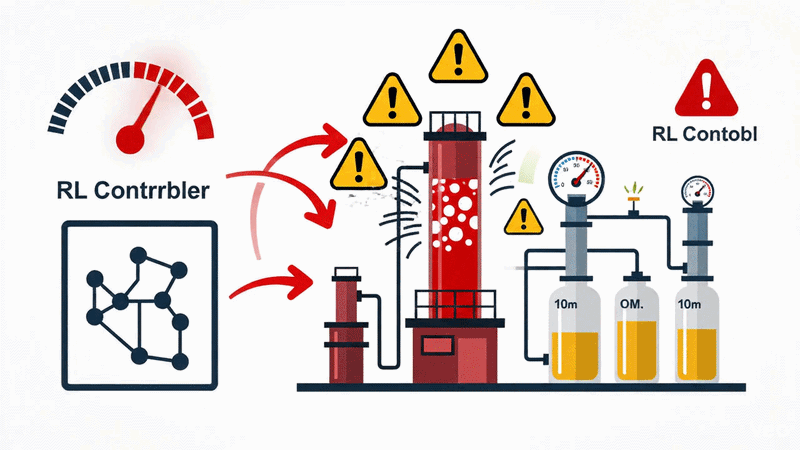
\includegraphics[
  width=0.96\linewidth,
  height=0.36\textheight,
  keepaspectratio,
  trim=10 8 10 16,
  clip
]{figures/rl-40.png}

\vspace{0.04cm}

{\tiny \textbf{Figure:} exploration that is acceptable in simulation can create unsafe or off-spec transients on a real plant.}

\end{column}

\begin{column}{0.54\textwidth}

\begin{block}{Why direct online RL is difficult}
\begin{itemize}\justifying
  \setlength\itemsep{0.45ex}

  \item Process dynamics are slow, so data arrive in real operating time.

  \item Exploration can violate constraints, create off-spec product, and stress actuators.

  \item Plants cannot be reset after each poor trajectory, and delayed consequences make credit assignment harder.
\end{itemize}
\end{block}

\vspace{0.03cm}

\begin{block}{Implication for this talk}
\begin{itemize}\justifying
  \setlength\itemsep{0.45ex}

  \item Direct online RL is not a realistic industrial baseline.

  \item Useful RL needs control structure, safer initialization, and a constrained role
  {\bf \color{maroon1} \scriptsize (Nian et al., 2020)}.
\end{itemize}
\end{block}

\end{column}

\end{columns}

\takeawaybox{The practical question is not how to explore freely online, but how to make RL learn within a constrained control structure.}

\end{frame}

%============================= Slide 7 ============================
\begin{frame}
\setbeamertemplate{blocks}[default]
\setbeamercolor{block body}{fg=black,bg=lightgray}
\frametitle{\large \textbf{There is a practical place for RL if it respects control structure}}
\scriptsize

\vspace{-0.23cm}

\begin{block}{Transition}
\justifying
The question is therefore not whether RL should replace process control, but where learning can help while keeping the controller practical, interpretable, and safe.
\end{block}

\vspace{0.02cm}

\begin{columns}[T,onlytextwidth]

\begin{column}{0.32\textwidth}
\begin{beamercolorbox}[wd=\linewidth,ht=3.0ex,dp=1.1ex,center,rounded=true]{pone title}
\scriptsize\textbf{1. MPC-pretrained RL}
\end{beamercolorbox}

\begin{beamercolorbox}[wd=\linewidth,sep=4pt,rounded=true]{pone body}
\begin{minipage}[t][0.45\textheight][t]{0.98\linewidth}
\centering

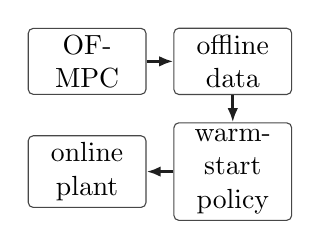
\begin{tikzpicture}[
  box/.style={draw=black!72,rounded corners=1.8pt,align=center,fill=white,inner sep=2.5pt,text width=1.32cm,minimum height=0.54cm},
  arrow/.style={-{Latex[length=1.8mm]},line width=0.95pt,draw=black!88}
]
\node[box] (mpc) at (0,0.85) {OF-MPC};
\node[box] (data) at (1.85,0.85) {offline\\data};
\node[box] (plant) at (0.0,-0.55) {online\\plant};
\node[box] (warm) at (1.85,-0.55) {warm-start\\policy};

\draw[arrow] (mpc) -- (data);
\draw[arrow] (data) -- (warm);
\draw[arrow] (warm) -- (plant);
\end{tikzpicture}

\vspace{0.6cm}

{\scriptsize \textbf{Role of RL}}\\[-0.1ex]
\tiny\justifying
RL starts from an MPC-like policy instead of unsafe random exploration.
\end{minipage}
\end{beamercolorbox}
\end{column}

\begin{column}{0.32\textwidth}
\begin{beamercolorbox}[wd=\linewidth,ht=3.0ex,dp=1.1ex,center,rounded=true]{ptwo title}
\scriptsize\textbf{2. RL-assisted MPC}
\end{beamercolorbox}

\begin{beamercolorbox}[wd=\linewidth,sep=4pt,rounded=true]{ptwo body}
\begin{minipage}[t][0.45\textheight][t]{0.98\linewidth}
\centering

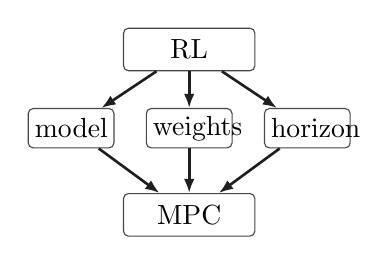
\begin{tikzpicture}[
  box/.style={draw=black!72,rounded corners=1.8pt,align=center,fill=white,inner sep=2.4pt,text width=0.92cm,minimum height=0.50cm},
  widebox/.style={draw=black!72,rounded corners=1.8pt,align=center,fill=white,inner sep=2.4pt,text width=1.50cm,minimum height=0.54cm},
  arrow/.style={-{Latex[length=1.8mm]},line width=0.95pt,draw=black!88}
]
\node[widebox] (rl) at (1.55,1.15) {RL};
\node[box] (model) at (0.05,0.15) {model};
\node[box] (weights) at (1.55,0.15) {weights};
\node[box] (horizon) at (3.05,0.15) {horizon};
\node[widebox] (mpc) at (1.55,-0.95) {MPC};

\draw[arrow] (rl) -- (model);
\draw[arrow] (rl) -- (weights);
\draw[arrow] (rl) -- (horizon);
\draw[arrow] (model) -- (mpc);
\draw[arrow] (weights) -- (mpc);
\draw[arrow] (horizon) -- (mpc);
\end{tikzpicture}

\vspace{0.2cm}

{\scriptsize \textbf{Role of RL}}\\[-0.1ex]
\tiny\justifying
RL helps MPC adapt without discarding the MPC optimizer.
\end{minipage}
\end{beamercolorbox}
\end{column}

\begin{column}{0.32\textwidth}
\begin{beamercolorbox}[wd=\linewidth,ht=3.0ex,dp=1.1ex,center,rounded=true]{pthree title}
\scriptsize\textbf{3. Direct Lyapunov gate}
\end{beamercolorbox}

\begin{beamercolorbox}[wd=\linewidth,sep=4pt,rounded=true]{pthree body}
\begin{minipage}[t][0.45\textheight][t]{0.98\linewidth}
\centering

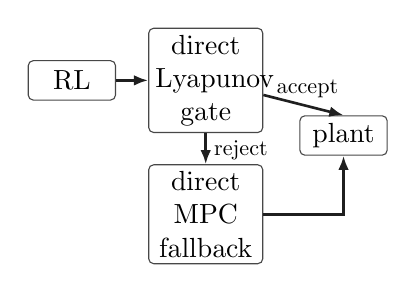
\begin{tikzpicture}[
  box/.style={draw=black!72,rounded corners=1.8pt,align=center,fill=white,inner sep=2.4pt,text width=0.94cm,minimum height=0.50cm},
  widebox/.style={draw=black!72,rounded corners=1.8pt,align=center,fill=white,inner sep=2.4pt,text width=1.28cm,minimum height=0.54cm},
  arrow/.style={-{Latex[length=1.8mm]},line width=0.95pt,draw=black!88}
]
\node[box] (rl) at (0,0.75) {RL};
\node[widebox] (check) at (1.70,0.75) {direct\\Lyapunov gate};
\node[box] (plant) at (3.45,0.05) {plant};
\node[widebox] (backup) at (1.70,-0.95) {direct MPC\\fallback};

\draw[arrow] (rl) -- (check);
\draw[arrow] (check) -- node[above,scale=0.80,pos=0.55] {accept} (plant.north);
\draw[arrow] (check) -- node[right,scale=0.80,pos=0.55] {reject} (backup);
\draw[arrow] (backup.east) -| (plant.south);
\end{tikzpicture}

\vspace{0.35cm}

{\scriptsize \textbf{Role of RL}}\\[-0.1ex]
\tiny\justifying
RL is used only when the candidate action already satisfies the direct Lyapunov contraction test.
\end{minipage}
\end{beamercolorbox}
\end{column}

\end{columns}

\end{frame}

%============================= Slide 8 ============================
\begin{frame}
\setbeamertemplate{blocks}[default]
\setbeamercolor{block body}{fg=black,bg=lightgray}
\frametitle{\large \textbf{The Aspen Dynamics \(C_2\) splitter is the motivating industrial problem}}
\scriptsize

\begin{columns}[T,onlytextwidth]
\begin{column}{0.43\textwidth}
\centering
\vspace{0.5cm}
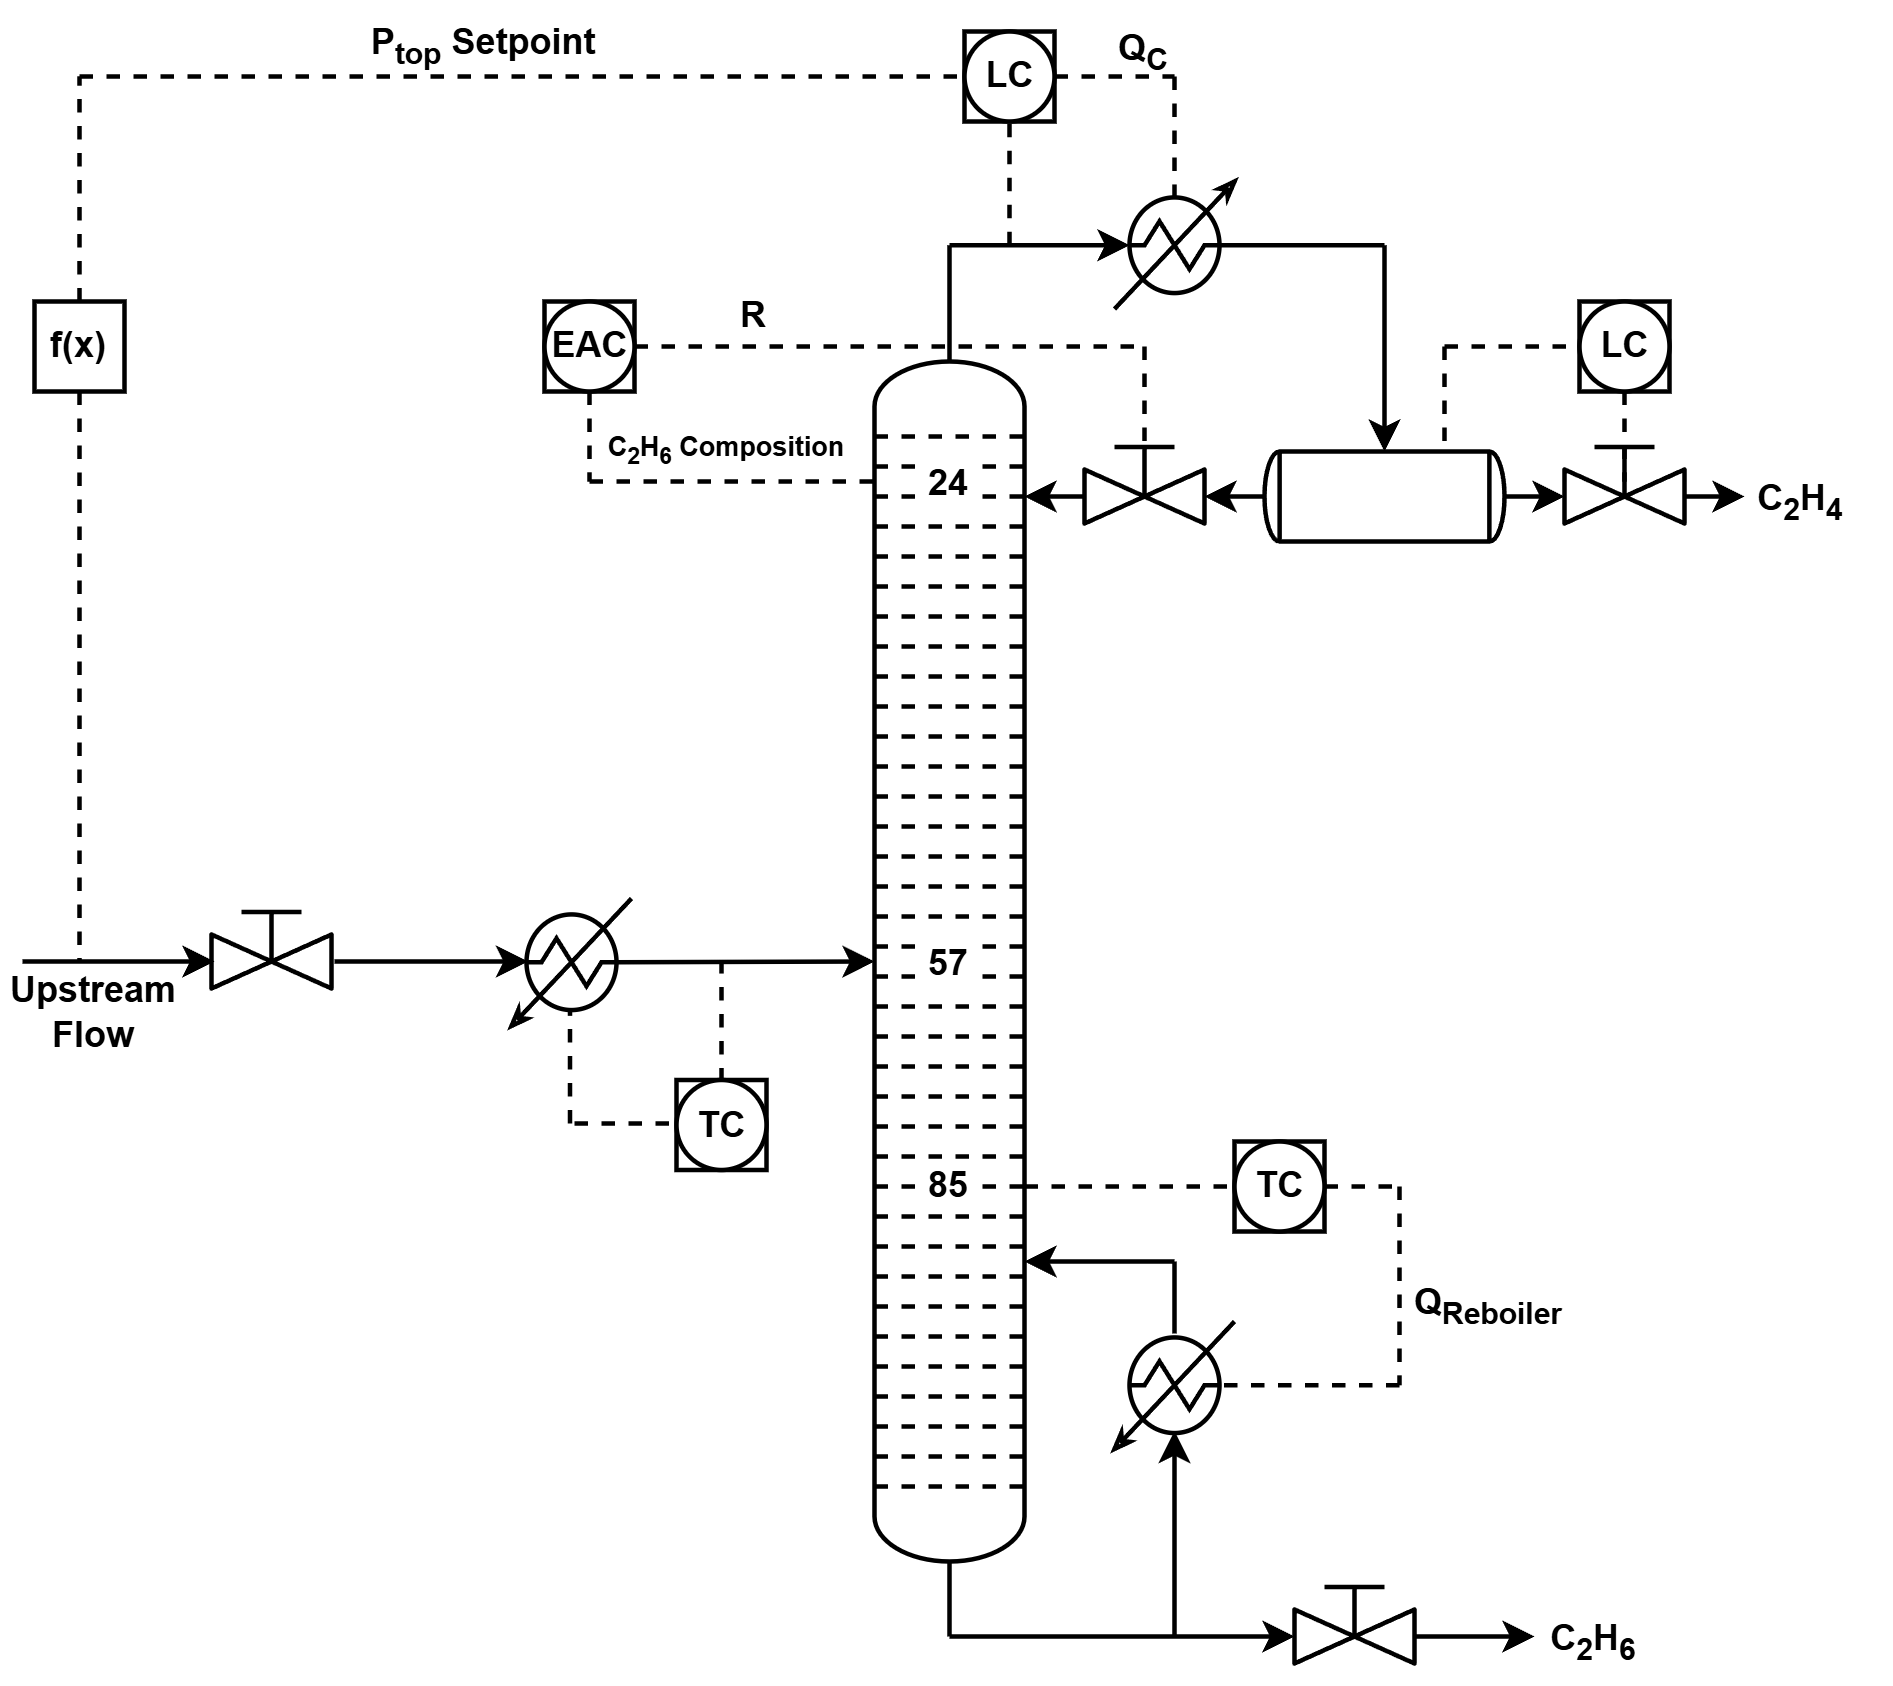
\includegraphics[width=0.94\linewidth]{figures/Distillation Column Overview.png}

\vspace{0.06cm}
{\scriptsize \textbf{Figure:} process diagram of the ethylene splitter used as the industrial-scale case study.}
\end{column}

\begin{column}{0.54\textwidth}
\begin{block}{Why this case study matters}
\begin{itemize}\justifying
  \item The \(C_2\) splitter is a high-purity ethylene separation with more than 100 trays, strong coupling, and expensive dynamics
  {\bf \color{maroon1} \scriptsize (Salerno et al., 2011)}.
  \item The control objective is tracking tray-24 ethane impurity \(x_{24,\mathrm{C_2H_6}}\) and tray-85 temperature \(T_{85}\) using reflux flow and reboiler duty.
\end{itemize}
\end{block}

\vspace{0.05cm}
\begin{block}{Why it is useful for this talk}
\begin{itemize}\justifying
  \item Aspen Dynamics is interfaced with Python, so the controller is tested on a high-fidelity closed loop rather than a toy simulator.
  \item A full closed-loop scenario is computationally expensive, so this case is used as the industrial-scale validation problem rather than the rapid method-development platform.
\end{itemize}
\end{block}
\end{column}
\end{columns}
\end{frame}

%============================= Slide 9 ============================
\begin{frame}
\setbeamertemplate{blocks}[default]
\setbeamercolor{block body}{fg=black,bg=lightgray}
\frametitle{\large \textbf{The polymer reactor is the illustrative benchmark for method development}}
\scriptsize

\begin{columns}[T,onlytextwidth]
\begin{column}{0.43\textwidth}
\centering
\vspace{1cm}
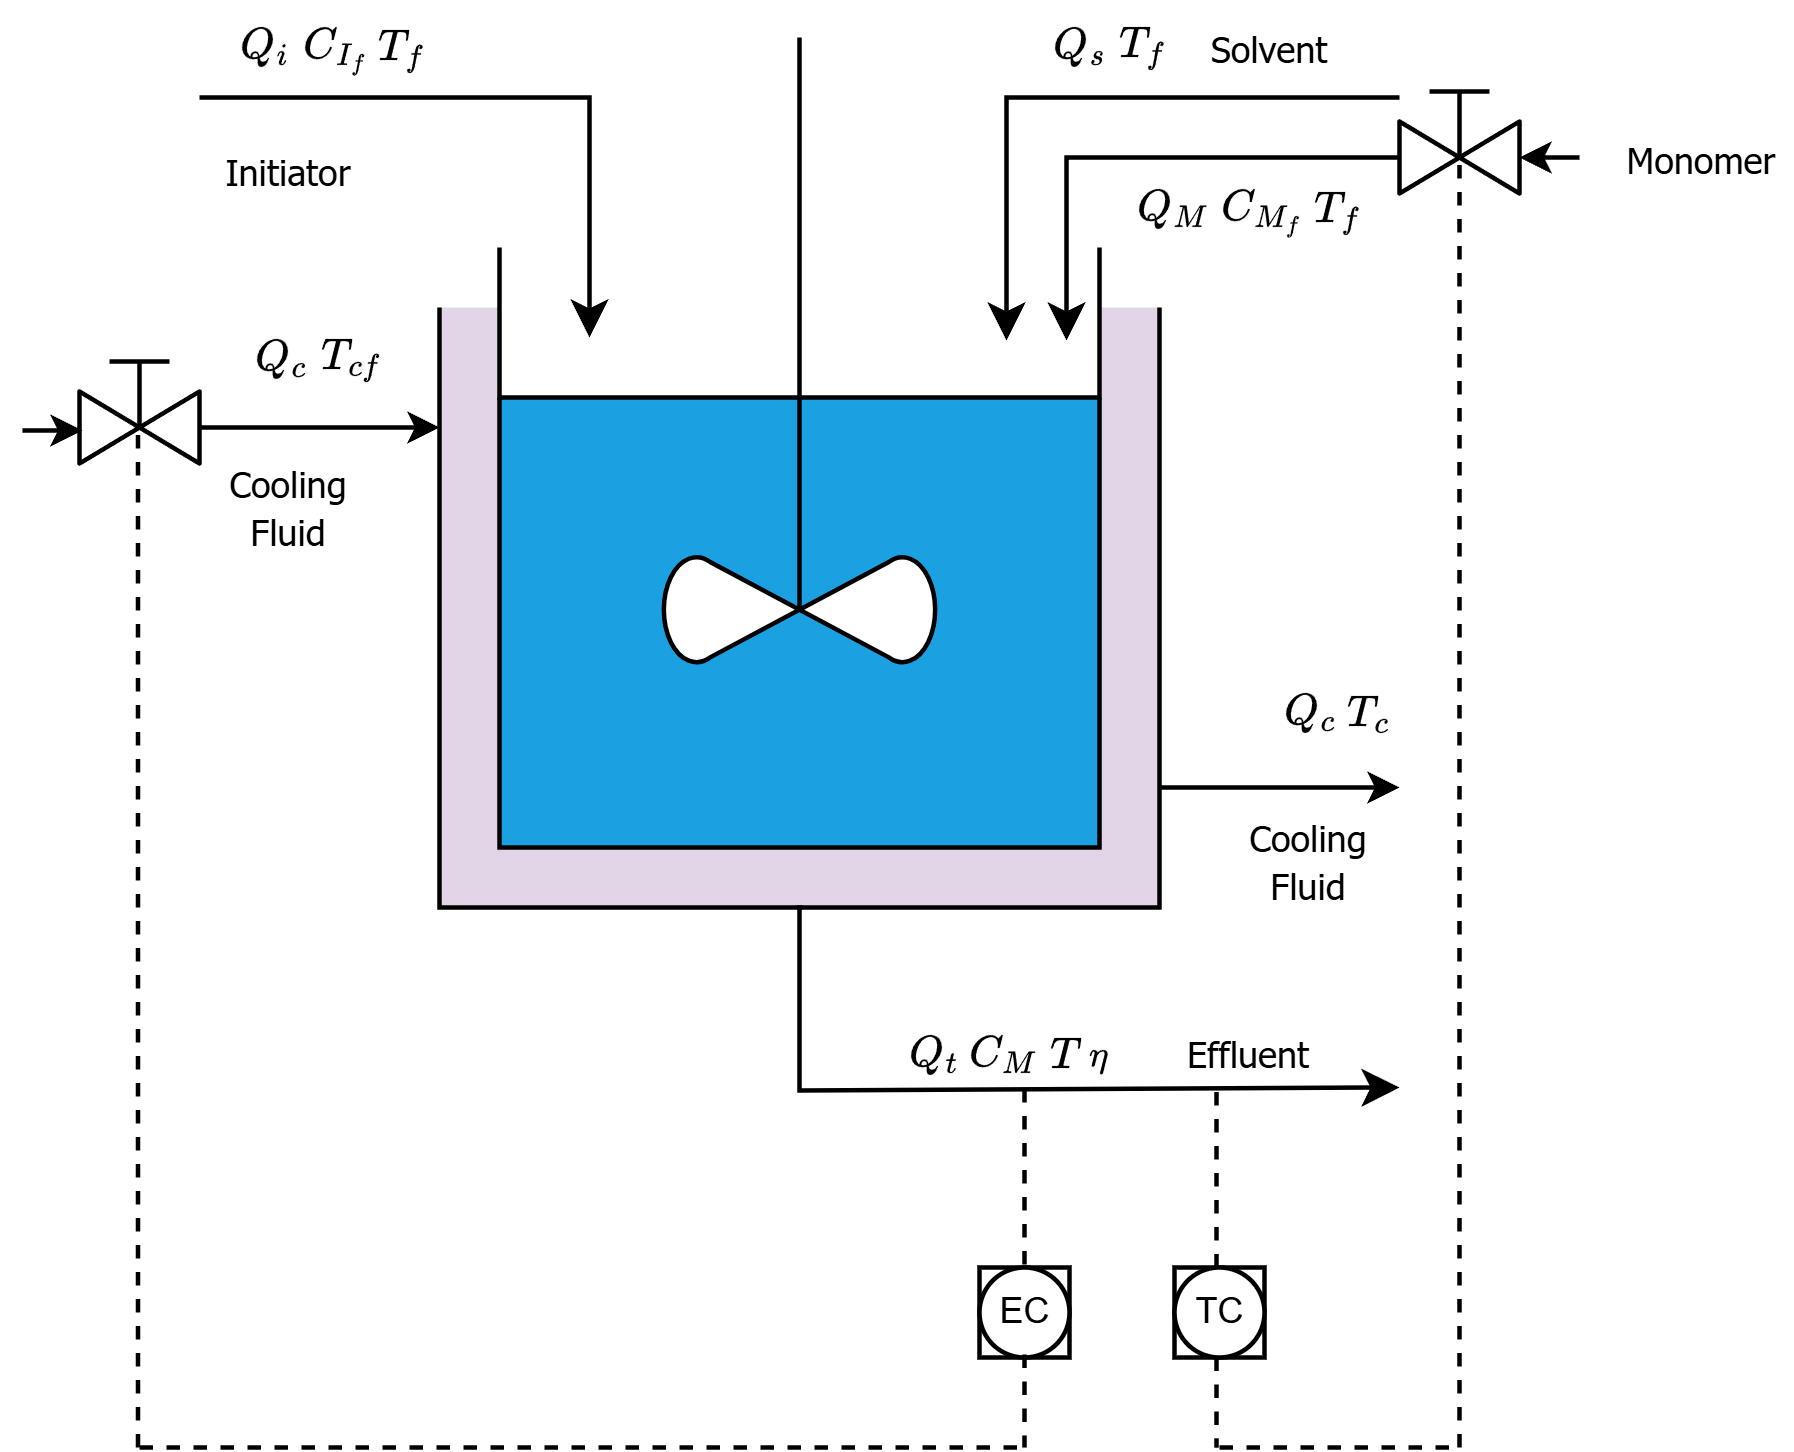
\includegraphics[width=0.82\linewidth]{figures/CSTR.png}

\vspace{0.06cm}
{\scriptsize \textbf{Figure:} styrene polymerization reactor used as the nonlinear MIMO benchmark in this work.}
\end{column}

\begin{column}{0.54\textwidth}
\begin{block}{Why this case study matters}
\begin{itemize}\justifying
  \item The reactor is nonlinear, strongly coupled, and constrained, so a fixed linear controller is only an approximation
  {\bf \color{maroon1} \scriptsize (Bustos et al., 2016)}.
  \item Manipulated inputs are the monomer flow rate \(Q_M\) and coolant flow rate \(Q_c\).
  \item Controlled outputs are intrinsic viscosity \(\eta\) and reactor temperature \(T\).
\end{itemize}
\end{block}

\vspace{0.05cm}
\begin{block}{Why it is useful for this talk}
\begin{itemize}\justifying
  \item In our current workflow, one closed-loop run is practical enough for repeated controller development, roughly on the order of one hour.
  \item Because closed-loop runs are much faster than the Aspen \(C_2\) case, the polymer reactor is used to debug learning behavior, reward design, and ablation studies before transfer to the industrial-scale system.
\end{itemize}
\end{block}
\end{column}
\end{columns}
\end{frame}

%============================= Slide 10 ============================
\begin{frame}
\setbeamertemplate{blocks}[default]
\setbeamercolor{block body}{fg=black,bg=lightgray}
\frametitle{\large \textbf{Project 1 starts from OF-MPC, so the actor is useful before online RL begins}}
\scriptsize

\vspace{-0.30cm}

\begin{columns}[T,onlytextwidth]

\begin{column}{0.41\textwidth}
\begin{block}{Practical idea}
\justifying
Use the controller already trusted in practice to create the initial RL policy, instead of beginning online learning from unsafe random actions.
\end{block}

\vspace{0.02cm}

\begin{block}{Offline transition generated from OF-MPC}
{\tiny
\vspace{-0.12cm}
\[
s_t=\begin{bmatrix}\tilde{x}_t\\ y_{SP}\\ u_{t-1}\end{bmatrix},
\quad
a_t=u_t^{\mathrm{MPC}},
\quad
s_{t+1}=\begin{bmatrix}\tilde{x}_{t+1}\\ y_{SP}\\ u_t^{\mathrm{MPC}}\end{bmatrix}
\]
\vspace{-0.26cm}
\[
r_t=-\Big(\|y_{t+1}-y_{SP}\|_Q^2+\|\Delta u_t\|_R^2\Big)
\]
}
\end{block}
\end{column}

\begin{column}{0.56\textwidth}
\centering
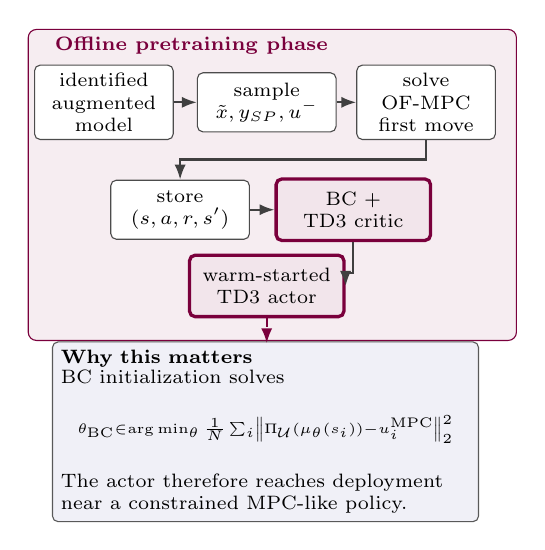
\begin{tikzpicture}[
  x=0.88cm,y=0.88cm,
  every node/.style={font=\scriptsize},
  phase/.style={draw=maroon1, rounded corners=3pt, fill=maroon1!7, inner sep=4pt},
  box/.style={draw=black!70, rounded corners=2pt, align=center, fill=white, inner sep=3pt, minimum height=0.75cm, text width=1.55cm},
  emph/.style={draw=maroon1, very thick, rounded corners=2pt, align=center, fill=maroon1!10, inner sep=3pt, minimum height=0.78cm, text width=1.75cm},
  note/.style={draw=black!65, rounded corners=2pt, align=left, fill=lightgray, inner sep=3pt, text width=5.2cm},
  arrow/.style={-{Latex[length=1.9mm]}, thick, draw=black!75},
  dasharrow/.style={-{Latex[length=1.9mm]}, thick, dashed, draw=maroon1}
]
\node[phase, minimum width=6.2cm, minimum height=3.95cm, anchor=north west] (offline) at (-0.25,2.16) {};
\node[anchor=west, font=\scriptsize\bfseries\color{maroon1}] at (0.00,1.92) {Offline pretraining phase};

\node[box] (model) at (0.85,1.10) {identified\\augmented model};
\node[box] (sample) at (3.2,1.10) {sample\\$\tilde{x},y_{SP},u^{-}$};
\node[box] (solve) at (5.5,1.10) {solve OF-MPC\\first move};
\node[box] (dataset) at (1.95,-0.45) {store\\$(s,a,r,s')$};
\node[emph] (actor) at (4.45,-0.45) {BC +\\TD3 critic};
\node[emph] (warm) at (3.20,-1.55) {warm-started\\TD3 actor};

\draw[arrow] (model) -- (sample);
\draw[arrow] (sample) -- (solve);
\draw[arrow] (solve.south) -- ++(0,-0.28) -| (dataset.north);
\draw[arrow] (dataset) -- (actor);
\draw[arrow] (actor.south) -- ++(+0, -0.45) -| (warm.east);

\node[note, anchor=north west] at (0.10,-2.35) {\textbf{Why this matters}\\[-0.3ex]
BC initialization solves
\[
{\scriptstyle
\theta_{\mathrm{BC}}\in
\arg\min_{\theta}
\frac{1}{N}\sum_i
\left\|
\Pi_{\mathcal U}(\mu_\theta(s_i))-u_i^{\mathrm{MPC}}
\right\|_2^2}
\]
The actor therefore reaches deployment near a constrained MPC-like policy.};

\draw[dasharrow] (warm.south) -- ++(0,-0.36);
\end{tikzpicture}
\end{column}

\end{columns}
\end{frame}

%============================= Slide 11 ============================
\begin{frame}
\setbeamertemplate{blocks}[default]
\setbeamercolor{block body}{fg=black,bg=lightgray}
\frametitle{\large \textbf{RL1 improves settling, but still leaves a small offset}}
\scriptsize

\vspace{-0.25cm}

\begin{columns}[T,onlytextwidth]

\begin{column}{0.60\textwidth}
\centering
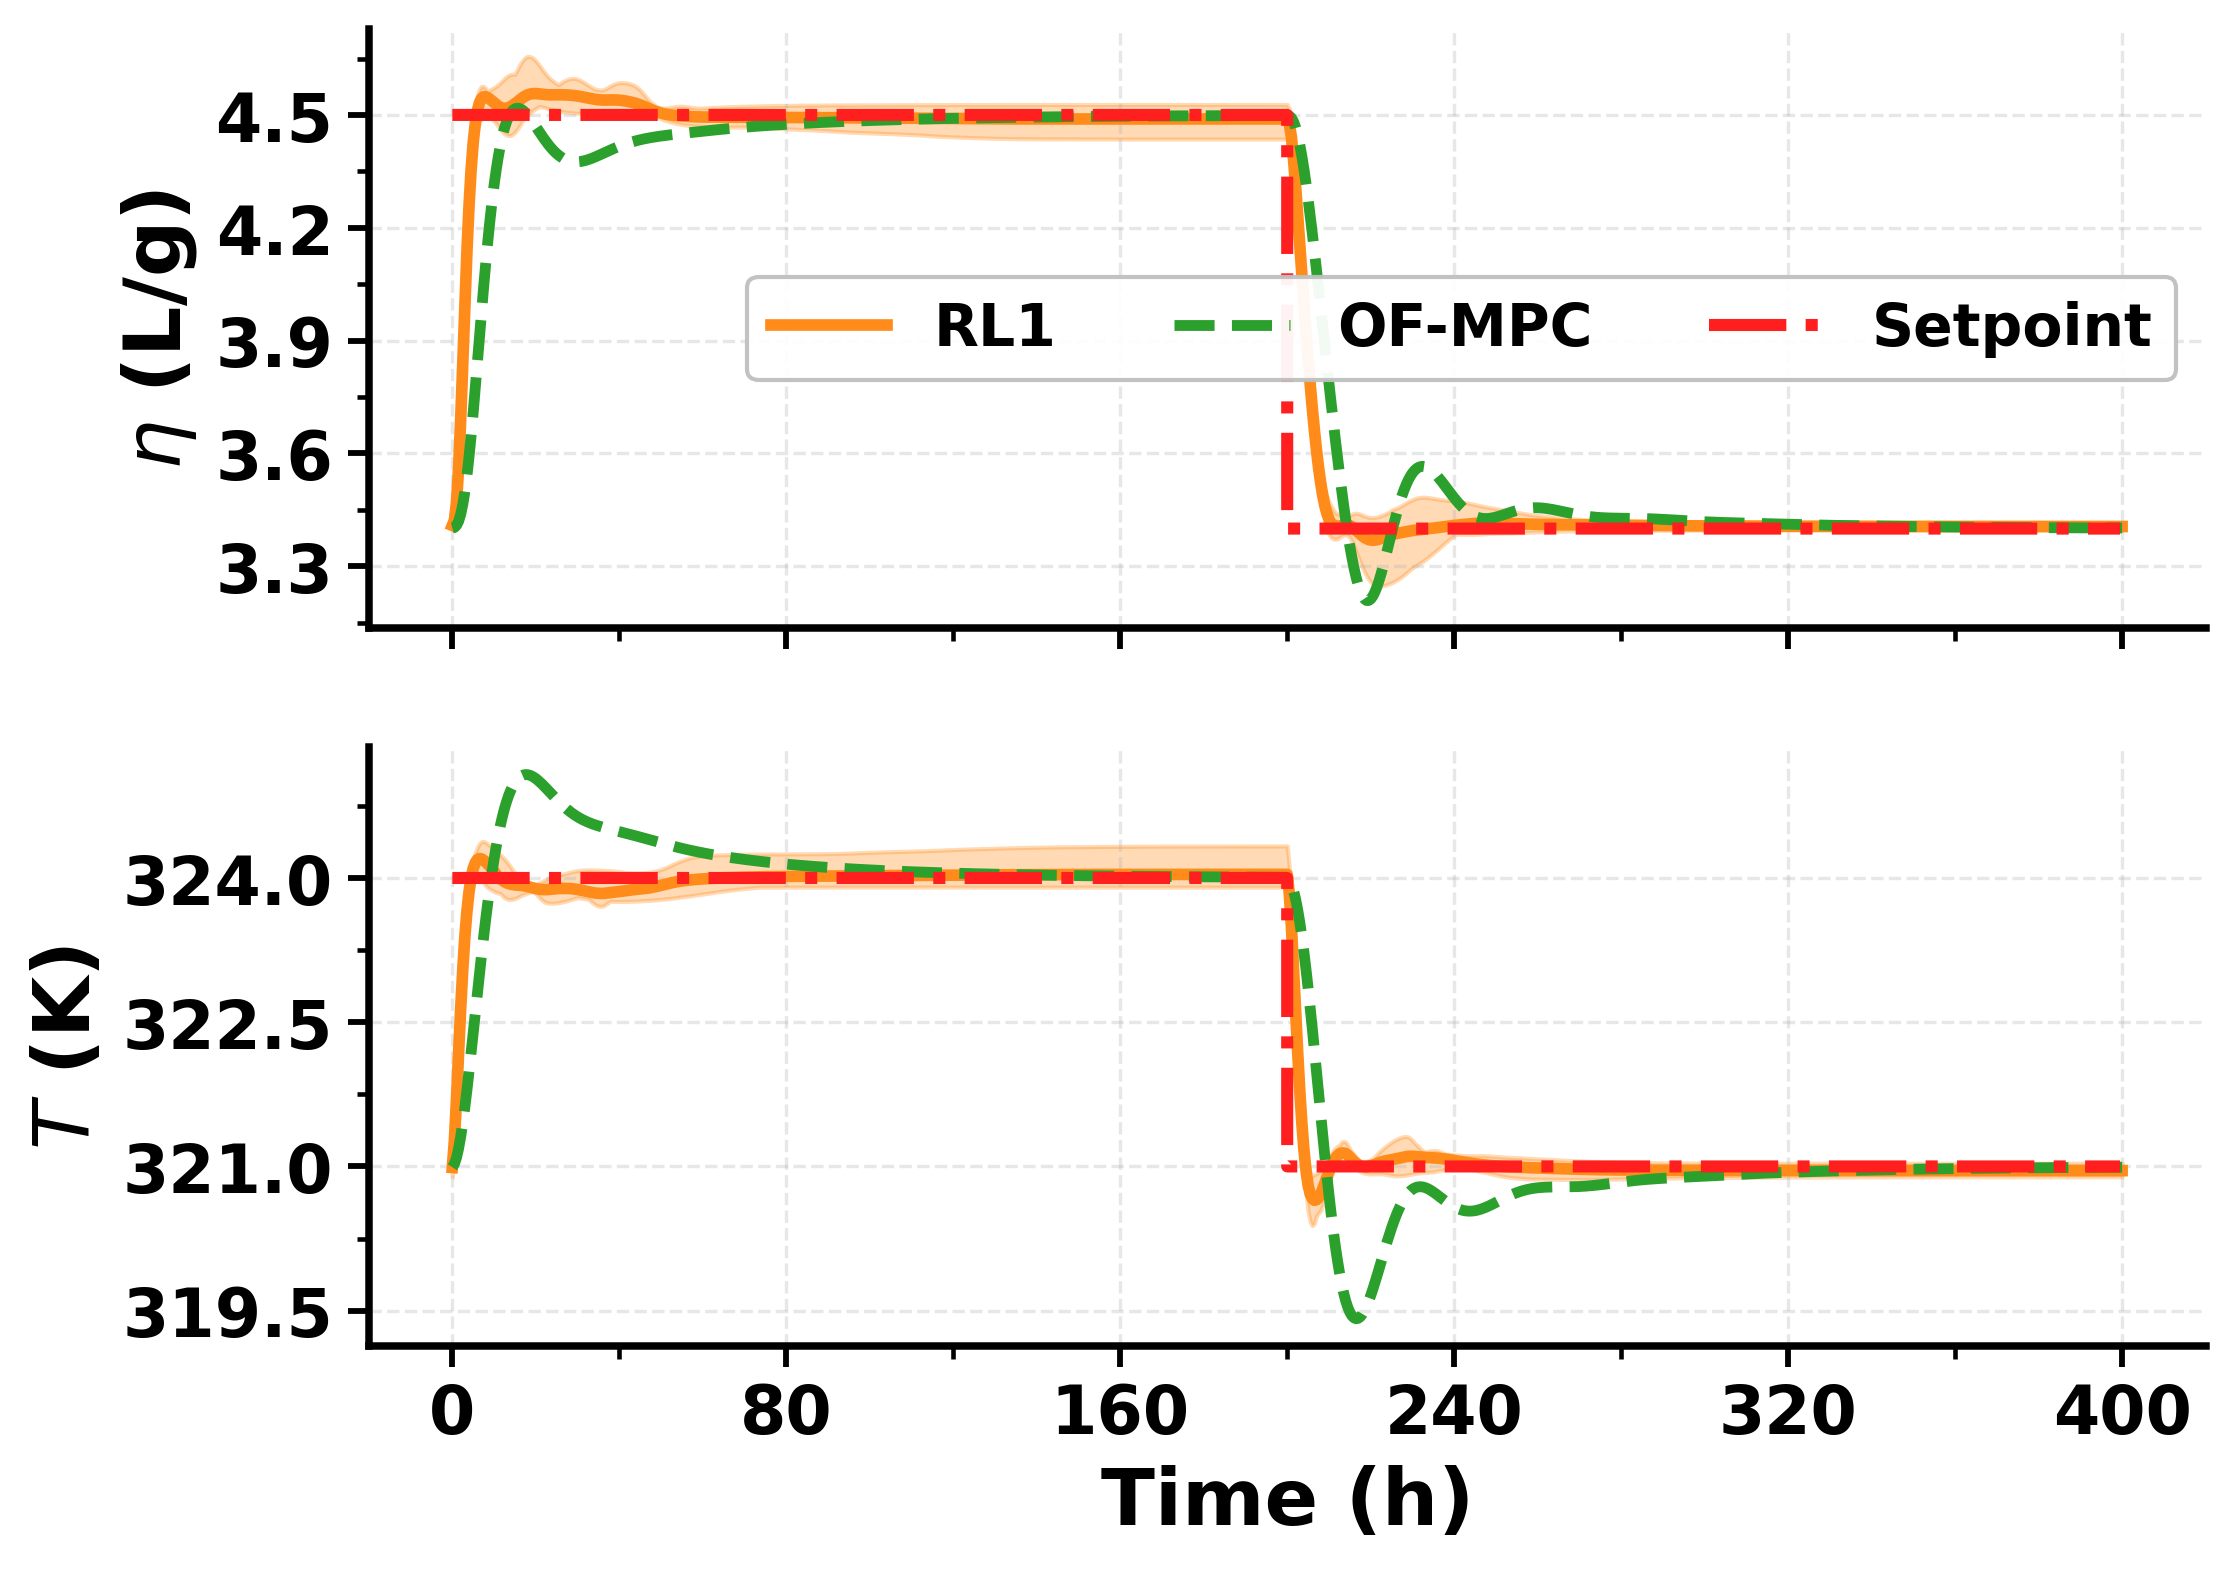
\includegraphics[width=0.96\linewidth]{figures/RL1_dist.png}

\vspace{0.03cm}
{\tiny \textbf{Figure:} RL1 settles faster than OF-MPC under operating changes, but a small final offset remains.}
\end{column}

\begin{column}{0.37\textwidth}

\begin{block}{RL1}
\justifying
Warm-started TD3 actor with the original one-step MPC-style reward
\[
r_t^{\mathrm{RL1}}
=
-\left(\|e_{t+1}\|_Q^2+\|\Delta u_t\|_R^2\right)
\]
\end{block}

\vspace{0.03cm}

\begin{block}{Main observation}
\begin{itemize}\justifying
  \setlength{\itemsep}{0.25em}
  \item Faster settling than OF-MPC
  \item Stable under drift
  \item Small residual offset remains
\end{itemize}
\end{block}

\end{column}

\end{columns}

\takeawaybox{Pretraining fixes initialization, but RL1 still under-emphasizes small final corrections near the setpoint.}

\end{frame}

%============================= Slide 12 ============================
\begin{frame}
\setbeamertemplate{blocks}[default]
\setbeamercolor{block body}{fg=black,bg=lightgray}
\frametitle{\large \textbf{RL2 changes the online learning signal, not the controller}}
\scriptsize
\setlength{\abovedisplayskip}{2pt}
\setlength{\belowdisplayskip}{2pt}
\vspace{-0.34cm}

\begin{columns}[T,onlytextwidth]

\begin{column}{0.53\textwidth}

\begin{block}{1. Offset-aware reward shaping}
\justifying
RL1 uses the one-step quadratic reward. RL2 increases sensitivity near the target using
\[
z_i=\frac{|e_i|}{b_i}
\]
so small residual offsets remain visible to TD3.
\end{block}

\vspace{0.00cm}
\centering
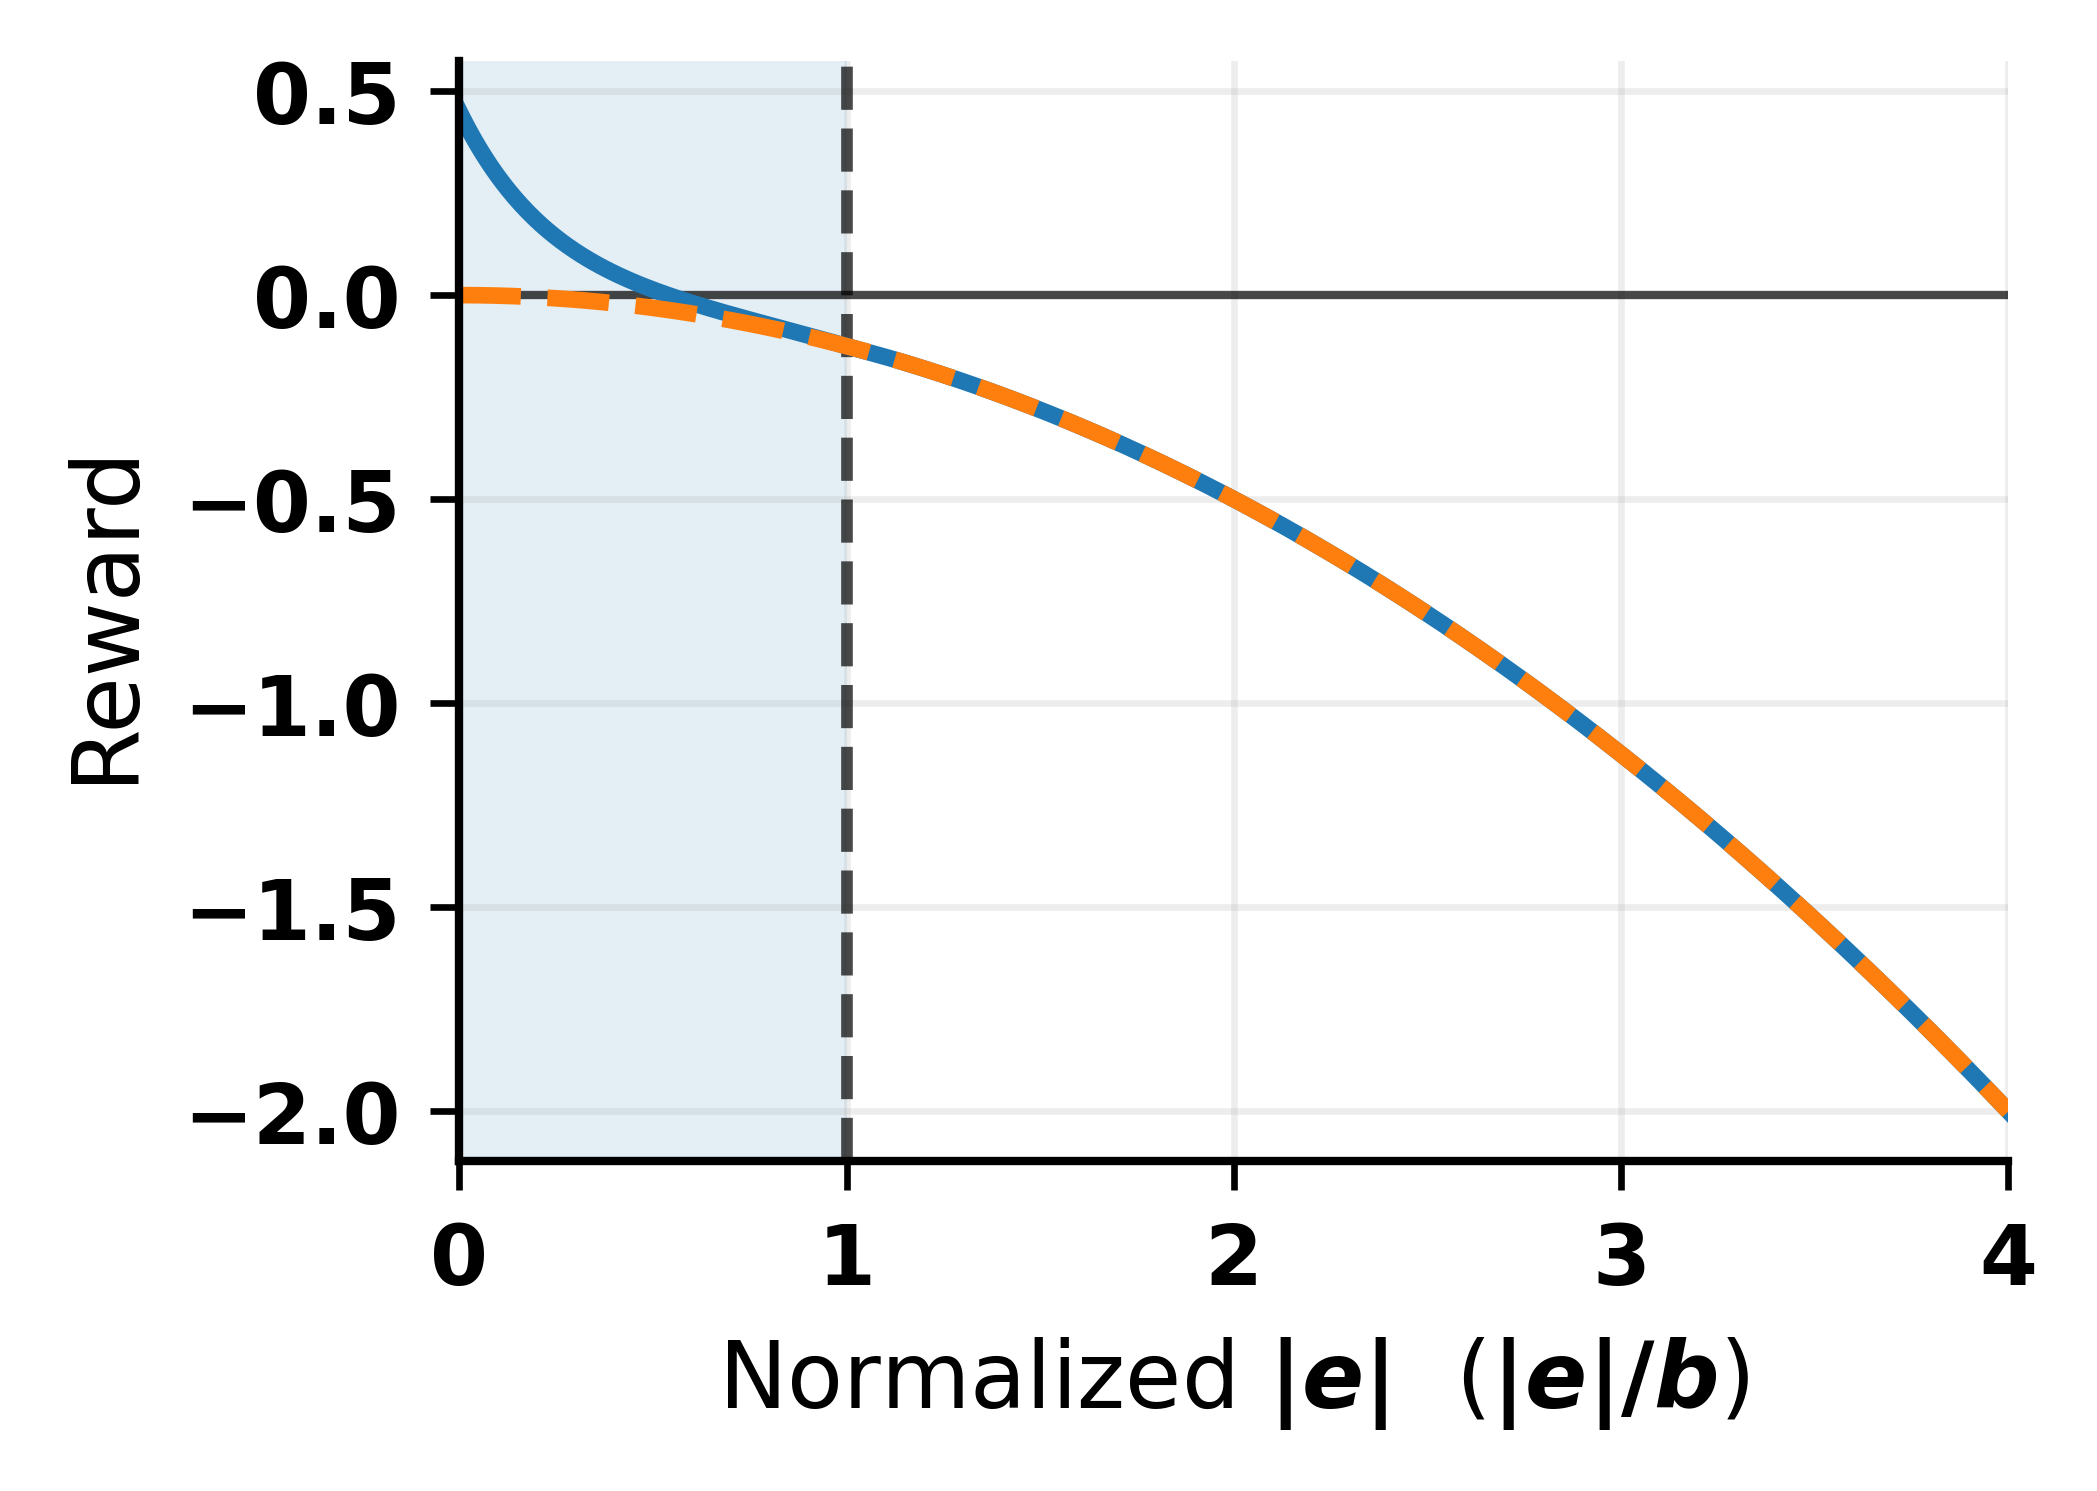
\includegraphics[width=0.5\linewidth,height=0.45\textheight,keepaspectratio]{figures/rewardplot_fn.png}

\vspace{0.01cm}

\begin{block}{2. Mixed replay for adaptation}
\justifying
Each batch mixes
\[
\mathcal B_{\mathrm{PER}}\cup\mathcal B_{\mathrm{recent}}\cup\mathcal B_{\mathrm{uniform}}
\]
so updates see informative errors, fresh drift data, and broad coverage.
\end{block}

\end{column}

\begin{column}{0.44\textwidth}

\begin{block}{Same TD3 backbone}
\justifying
\[
s_t=\begin{bmatrix}\hat{\tilde{x}}_t\\ y_{SP}\\ u_{t-1}\end{bmatrix},
\qquad
u_t=\Pi_{\mathcal U}\!\left(\mu_\theta(s_t)\right)
\]
\end{block}

\vspace{0.02cm}

\begin{block}{RL1 versus RL2}
\renewcommand{\arraystretch}{1.14}
\begin{tabular}{>{\raggedright\arraybackslash}p{0.19\linewidth} >{\raggedright\arraybackslash}p{0.66\linewidth}}
\textbf{RL1} & quadratic reward + standard replay \\
\textbf{RL2} & near-target reward + mixed replay \\
\textbf{Same} & warm start, observer, projection, TD3
\end{tabular}
\end{block}

\vspace{0.02cm}

\begin{beamercolorbox}[wd=\linewidth,sep=3pt,rounded=true]{takeawaybox}
\justifying
\textbf{Key point:} RL2 targets residual offset by changing what TD3 learns from, while keeping the same bounded actor.
\end{beamercolorbox}

\end{column}

\end{columns}

\end{frame}

%============================= Slide 13 ============================
\begin{frame}
\setbeamertemplate{blocks}[default]
\setbeamercolor{block body}{fg=black,bg=lightgray}
\frametitle{\large \textbf{On the polymer reactor, RL2 keeps the transient gain and reduces offset}}
\scriptsize
\vspace{-0.28cm}

\begin{columns}[T,onlytextwidth]

\begin{column}{0.57\textwidth}
\centering
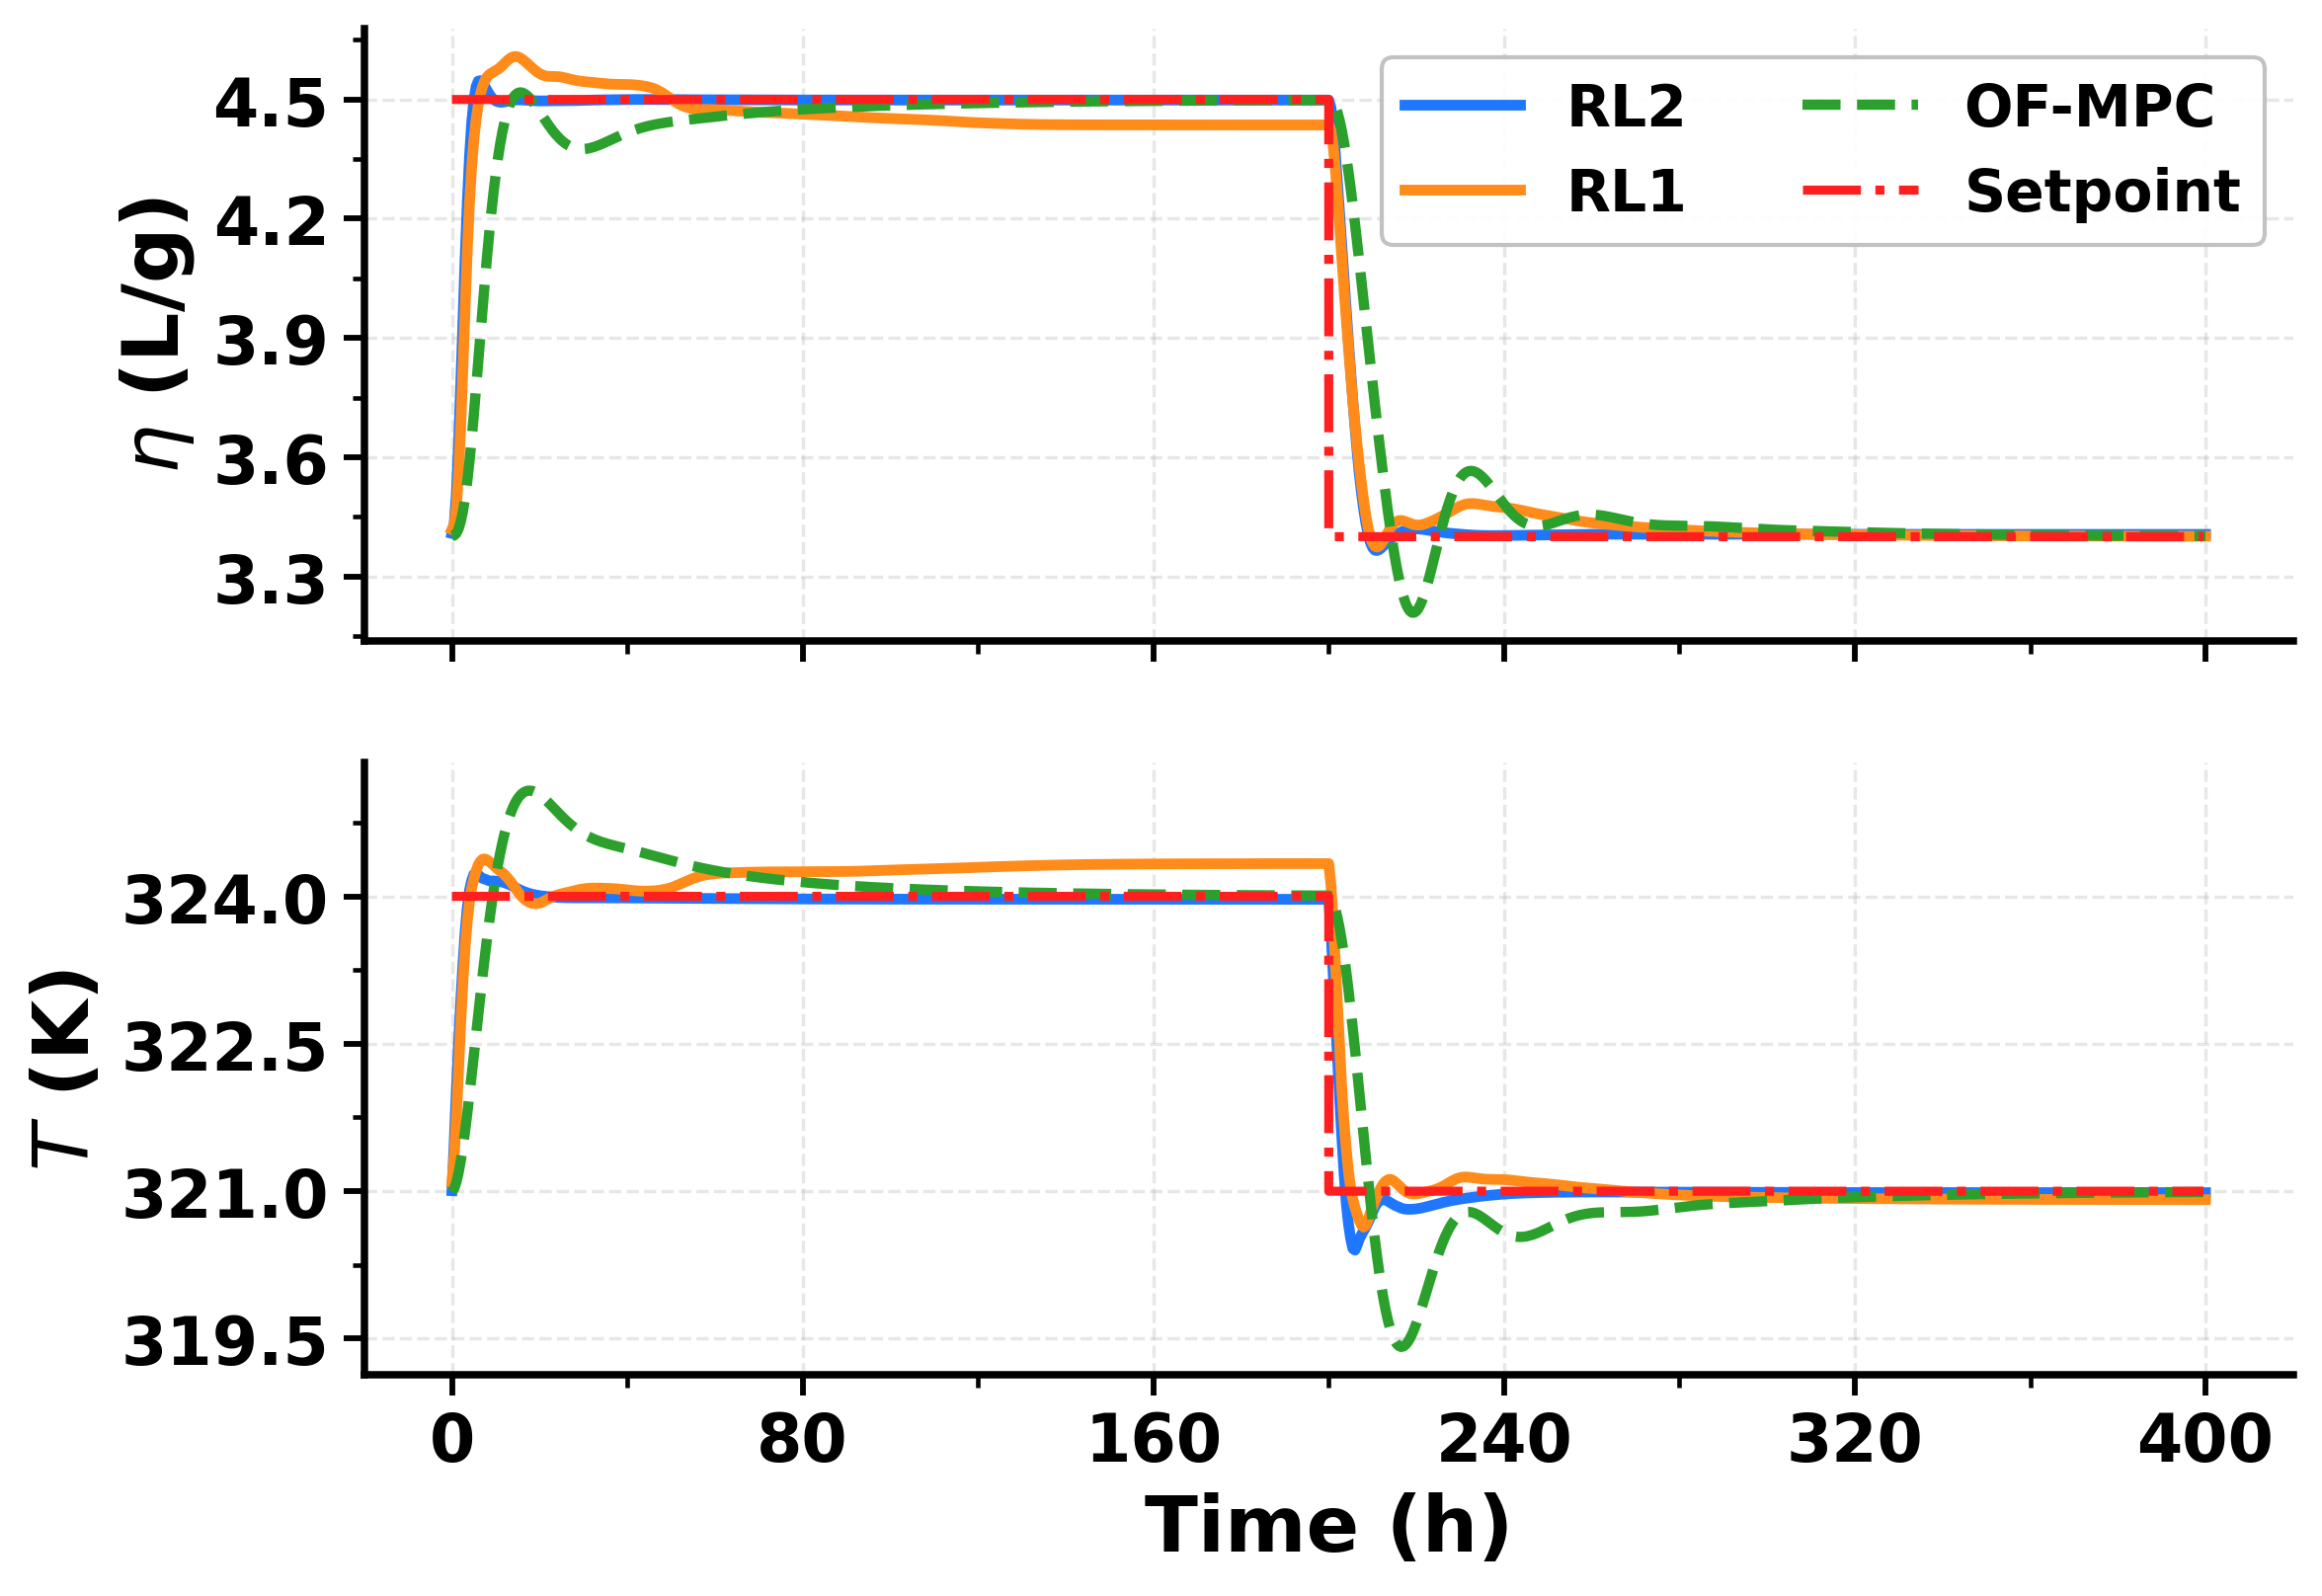
\includegraphics[width=\linewidth,height=0.54\textheight,keepaspectratio]{figures/compare_rl1_rl2_mpc_dist.png}

\vspace{0.02cm}
{\tiny \textbf{Figure:} evaluation under unseen operating changes. RL2 settles faster than OF-MPC and finishes closest to the setpoints.}
\end{column}

\begin{column}{0.40\textwidth}
\centering
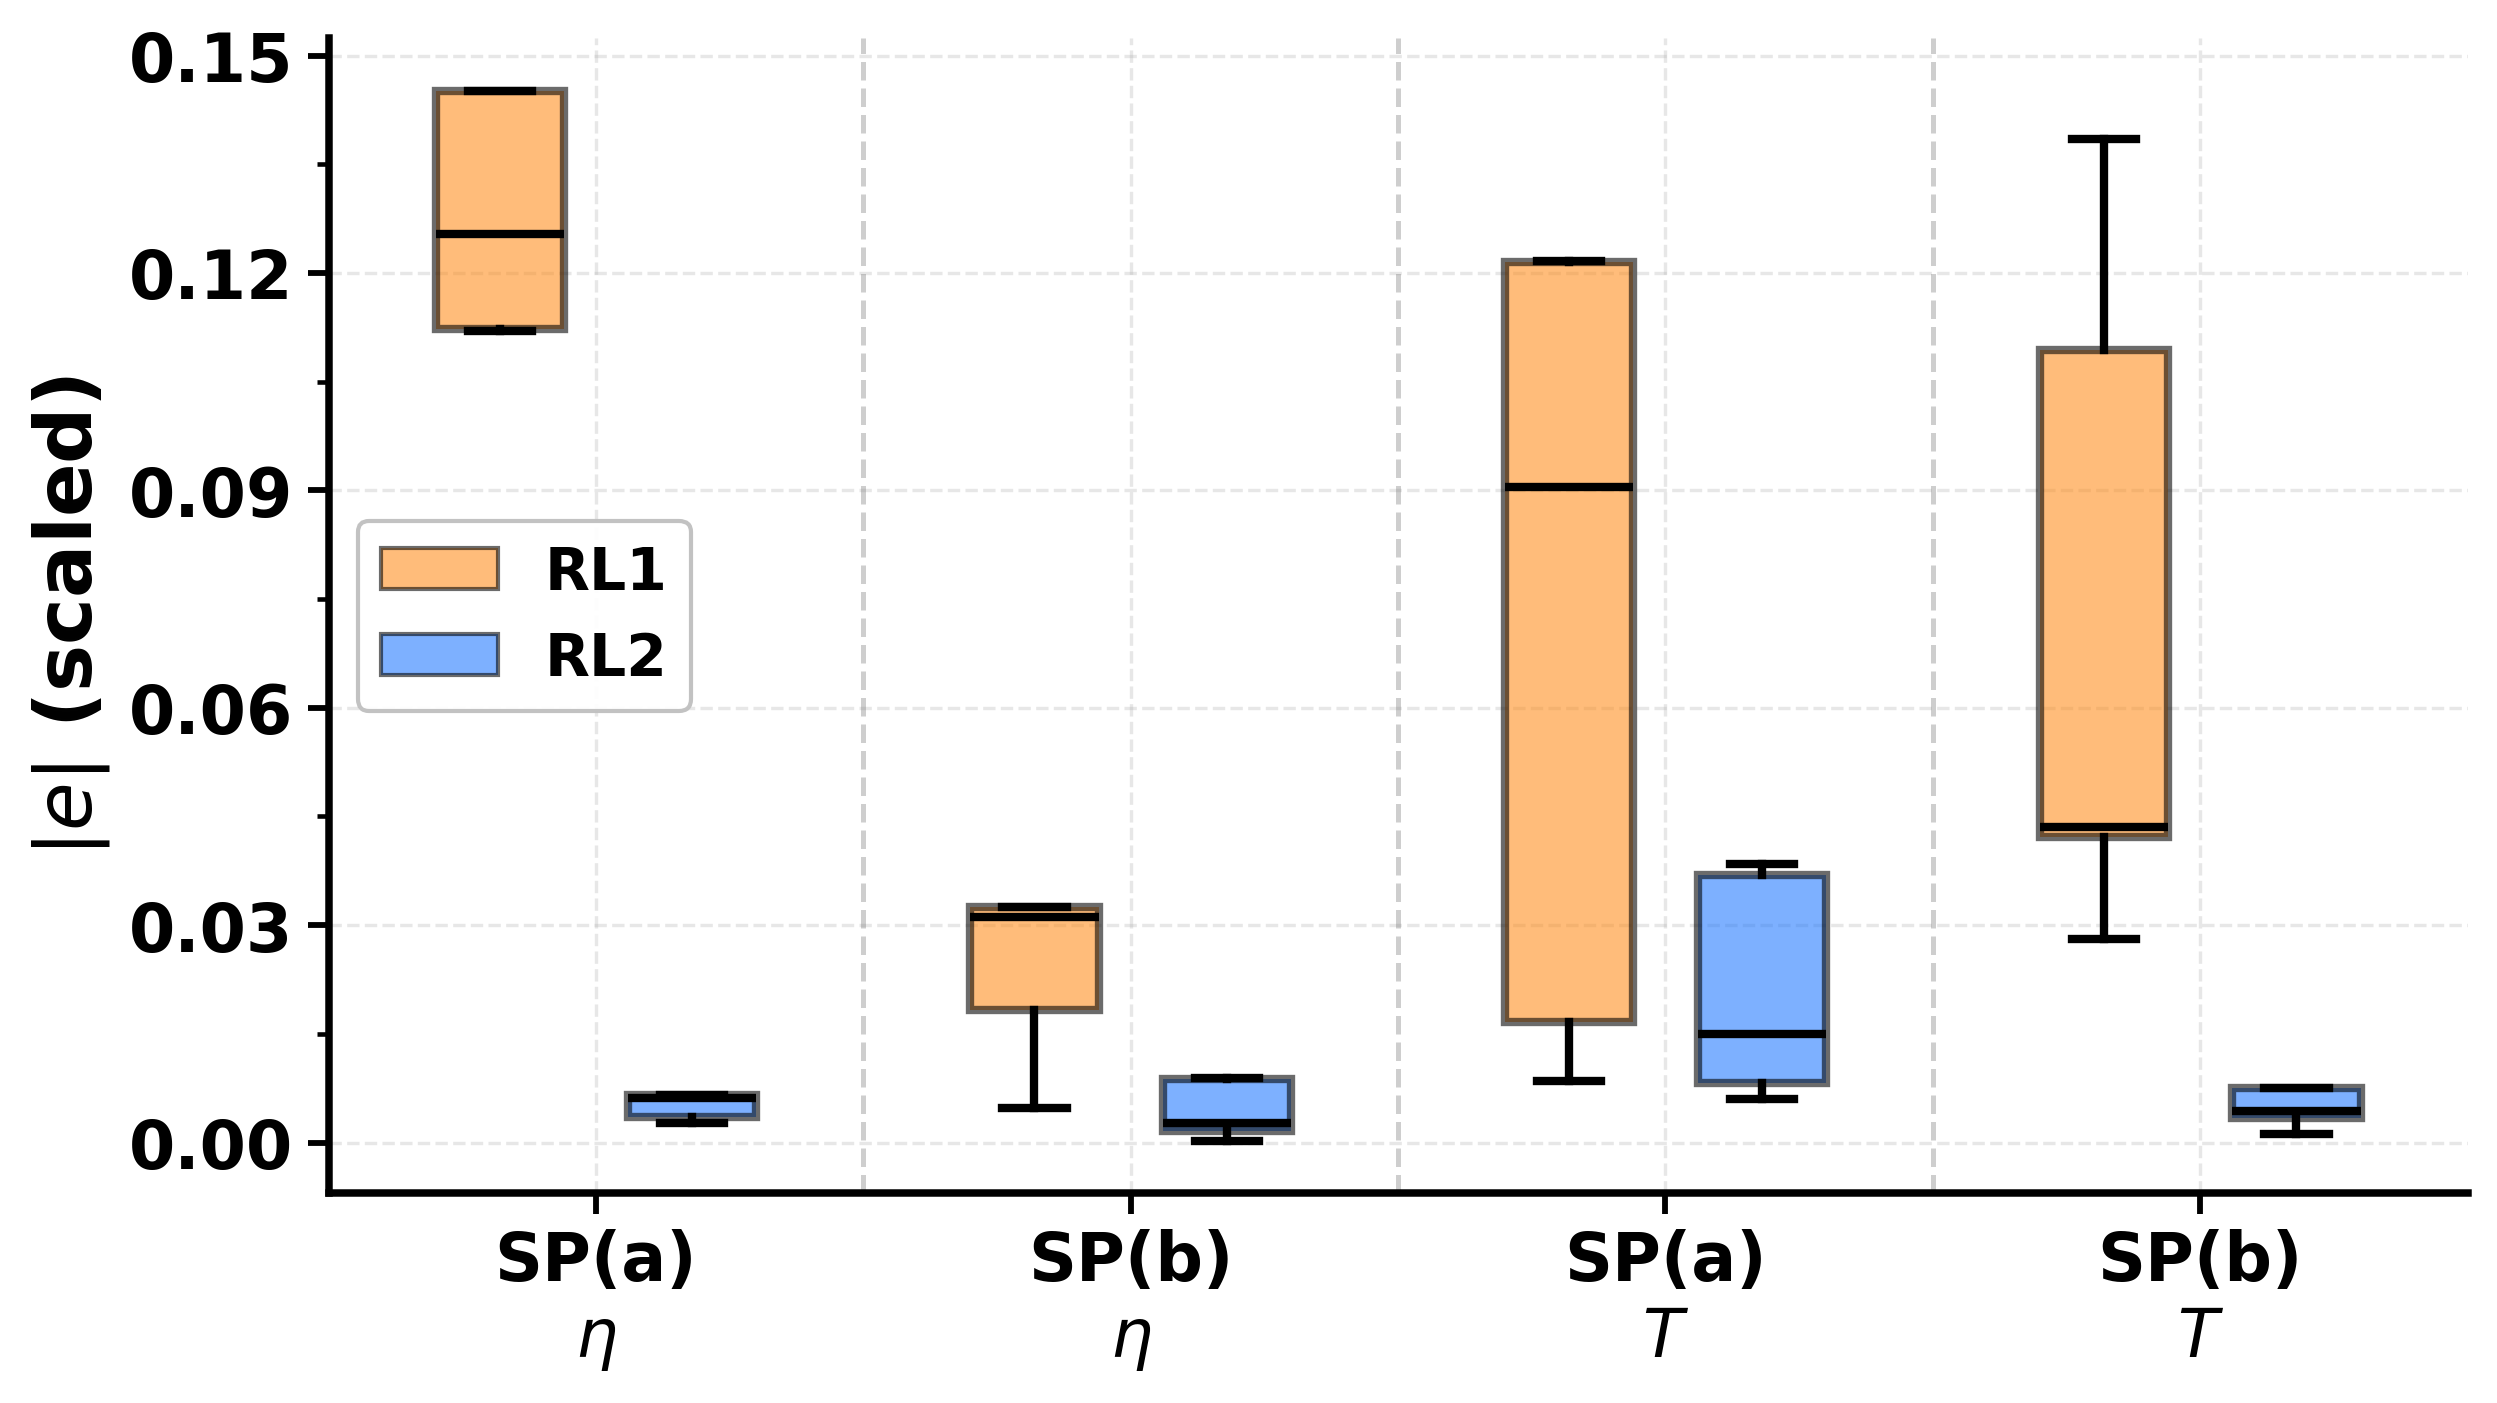
\includegraphics[width=0.96\linewidth,height=0.34\textheight,keepaspectratio]{figures/fig_box_abs_error_scaled_eval_last_dist.png}

\vspace{0.03cm}

\begin{block}{Error reduction vs RL1}
\centering
\renewcommand{\arraystretch}{1.16}
\begin{tabular}{c c c}
 & \textbf{SP(a)} & \textbf{SP(b)} \\
\(\eta\) & \textbf{92\%} & \textbf{76\%} \\
\(T\) & \textbf{84\%} & \textbf{90\%}
\end{tabular}
\end{block}

\vspace{0.02cm}

{\tiny Averaged over 5 runs, RL2 gives smaller medians and tighter spreads than RL1.}

\end{column}

\end{columns}

\end{frame}

%============================= Slide 14 ============================
\begin{frame}
\setbeamertemplate{blocks}[default]
\setbeamercolor{block body}{fg=black,bg=lightgray}
\frametitle{\large \textbf{On the Aspen \(C_2\) splitter, RL2 remains better in both scenarios}}
\scriptsize
\vspace{-0.30cm}

\begin{center}
\begin{minipage}[t]{0.48\textwidth}
\centering
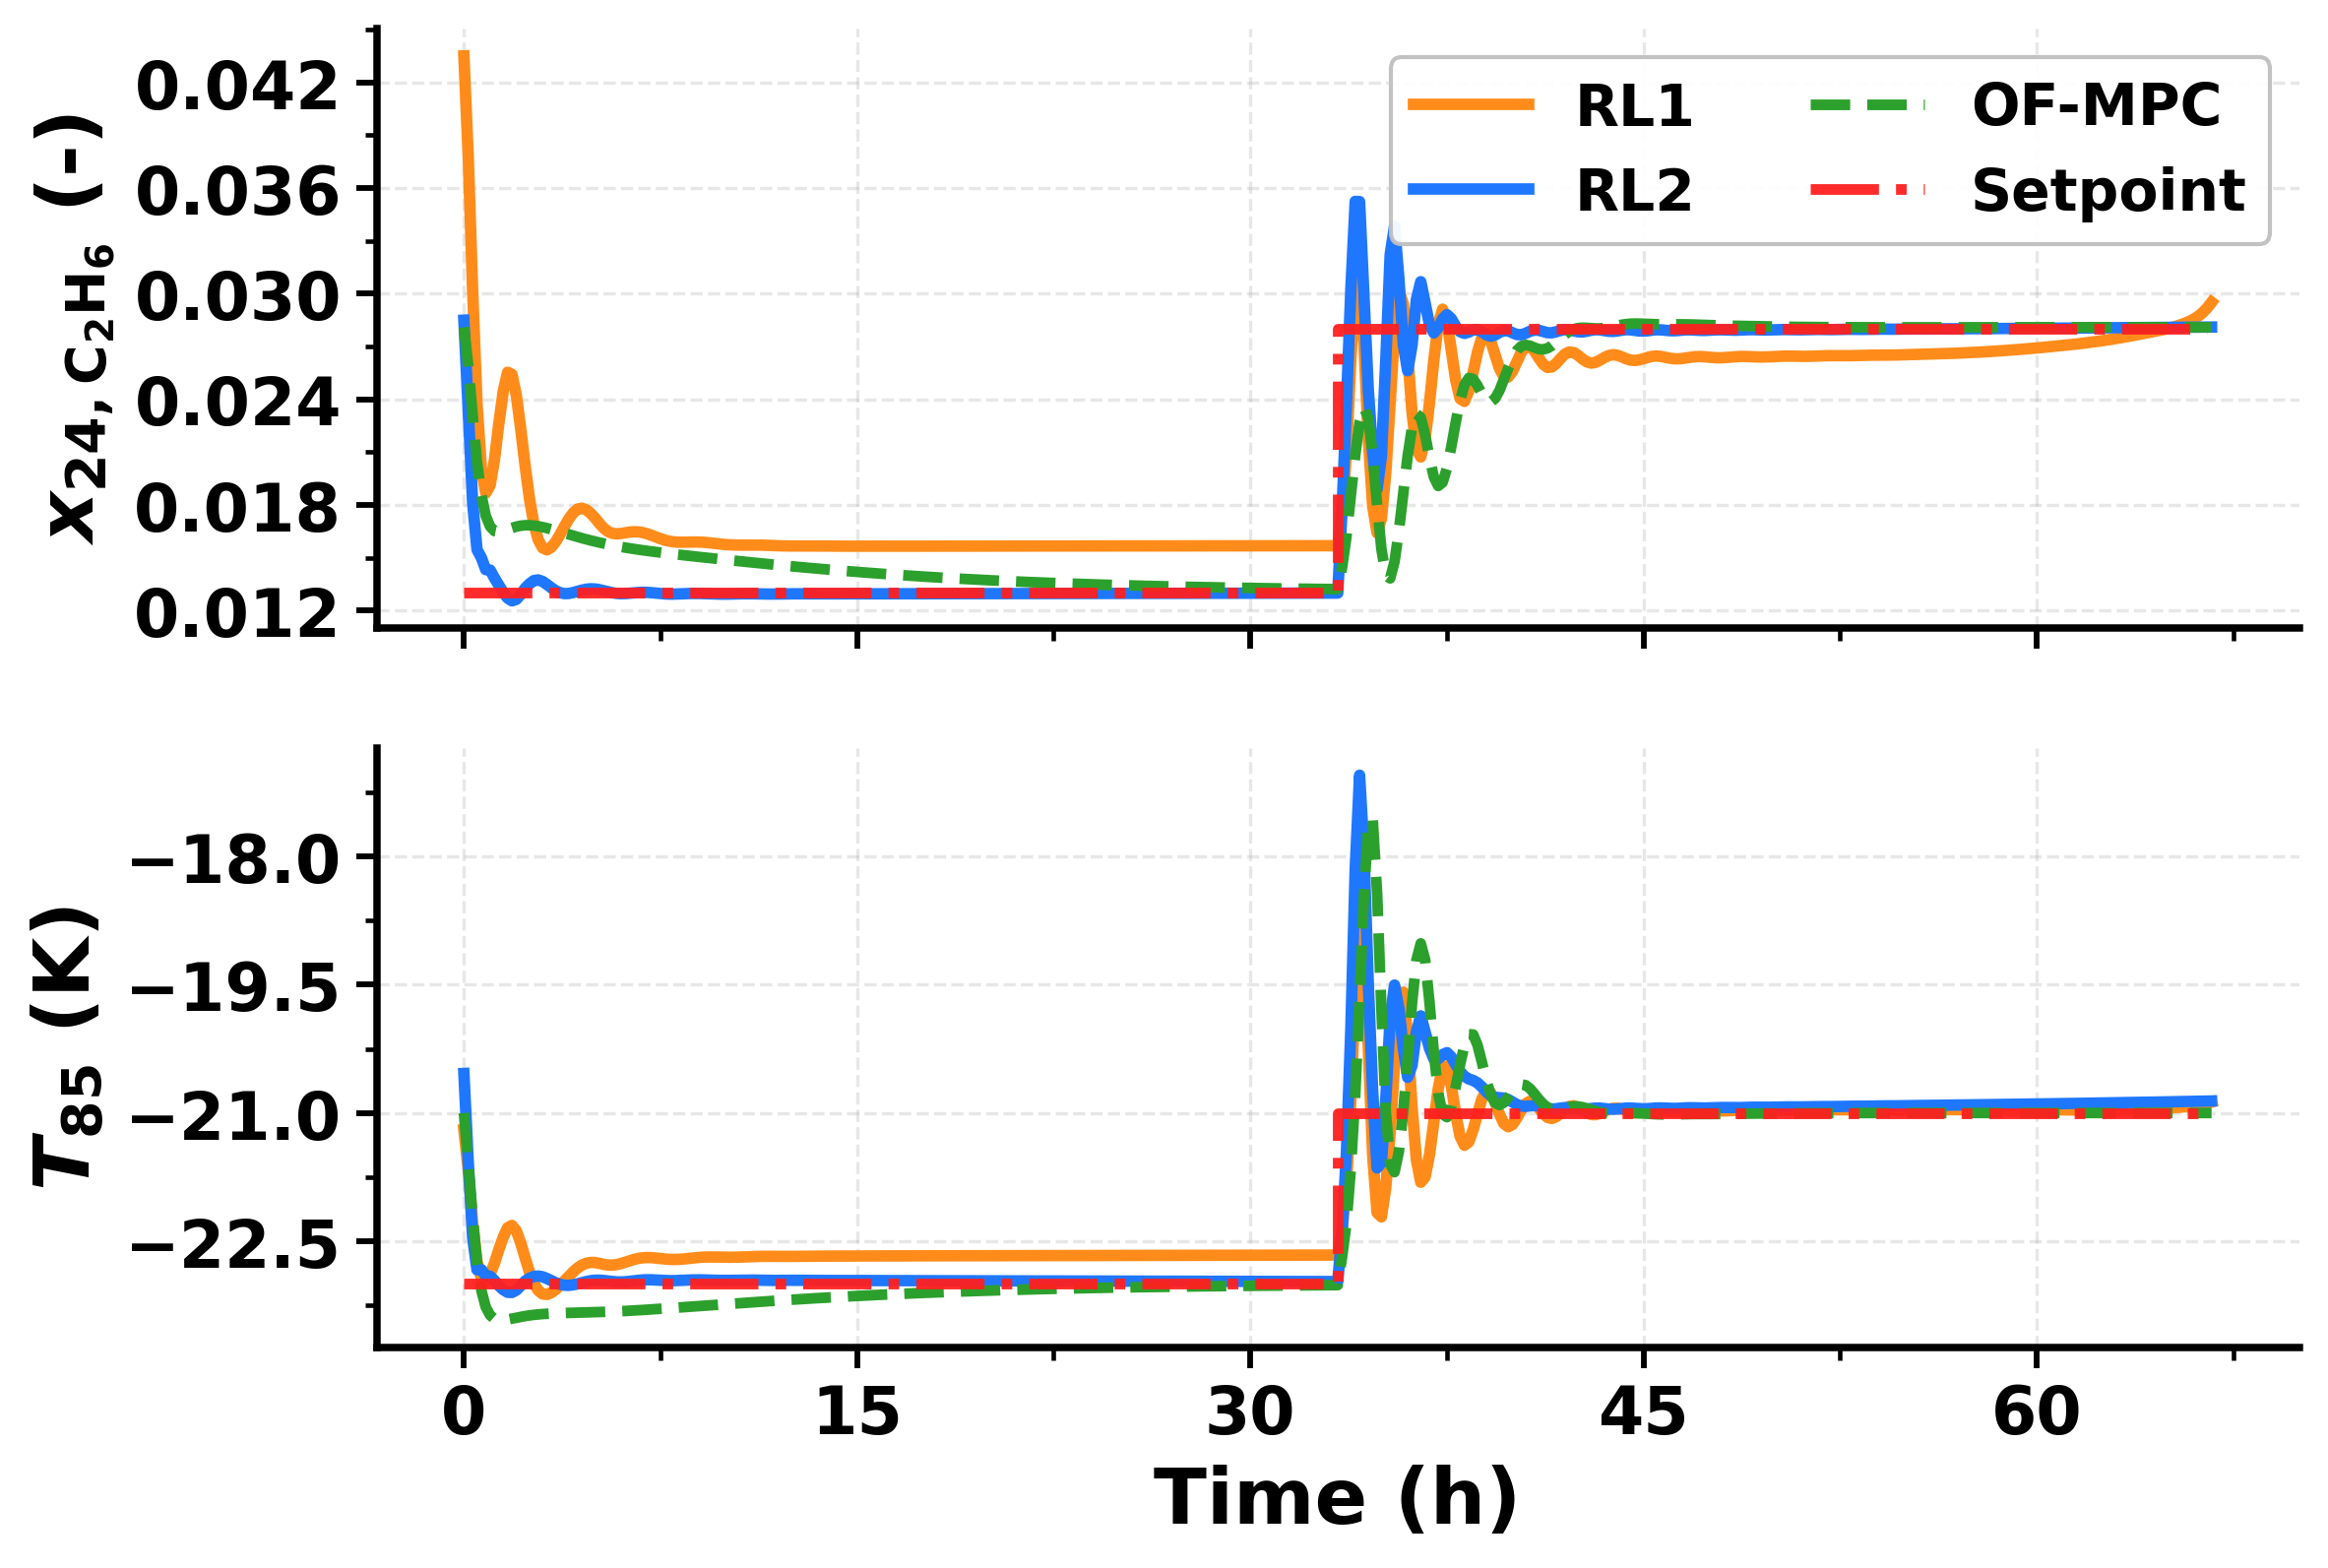
\includegraphics[width=\linewidth,height=0.48\textheight,keepaspectratio]{figures/C2_rampnoise_outputs_compare_three.png}

\vspace{0.01cm}
{\tiny \textbf{Fluctuation scenario}}
\end{minipage}
\hfill
\begin{minipage}[t]{0.48\textwidth}
\centering
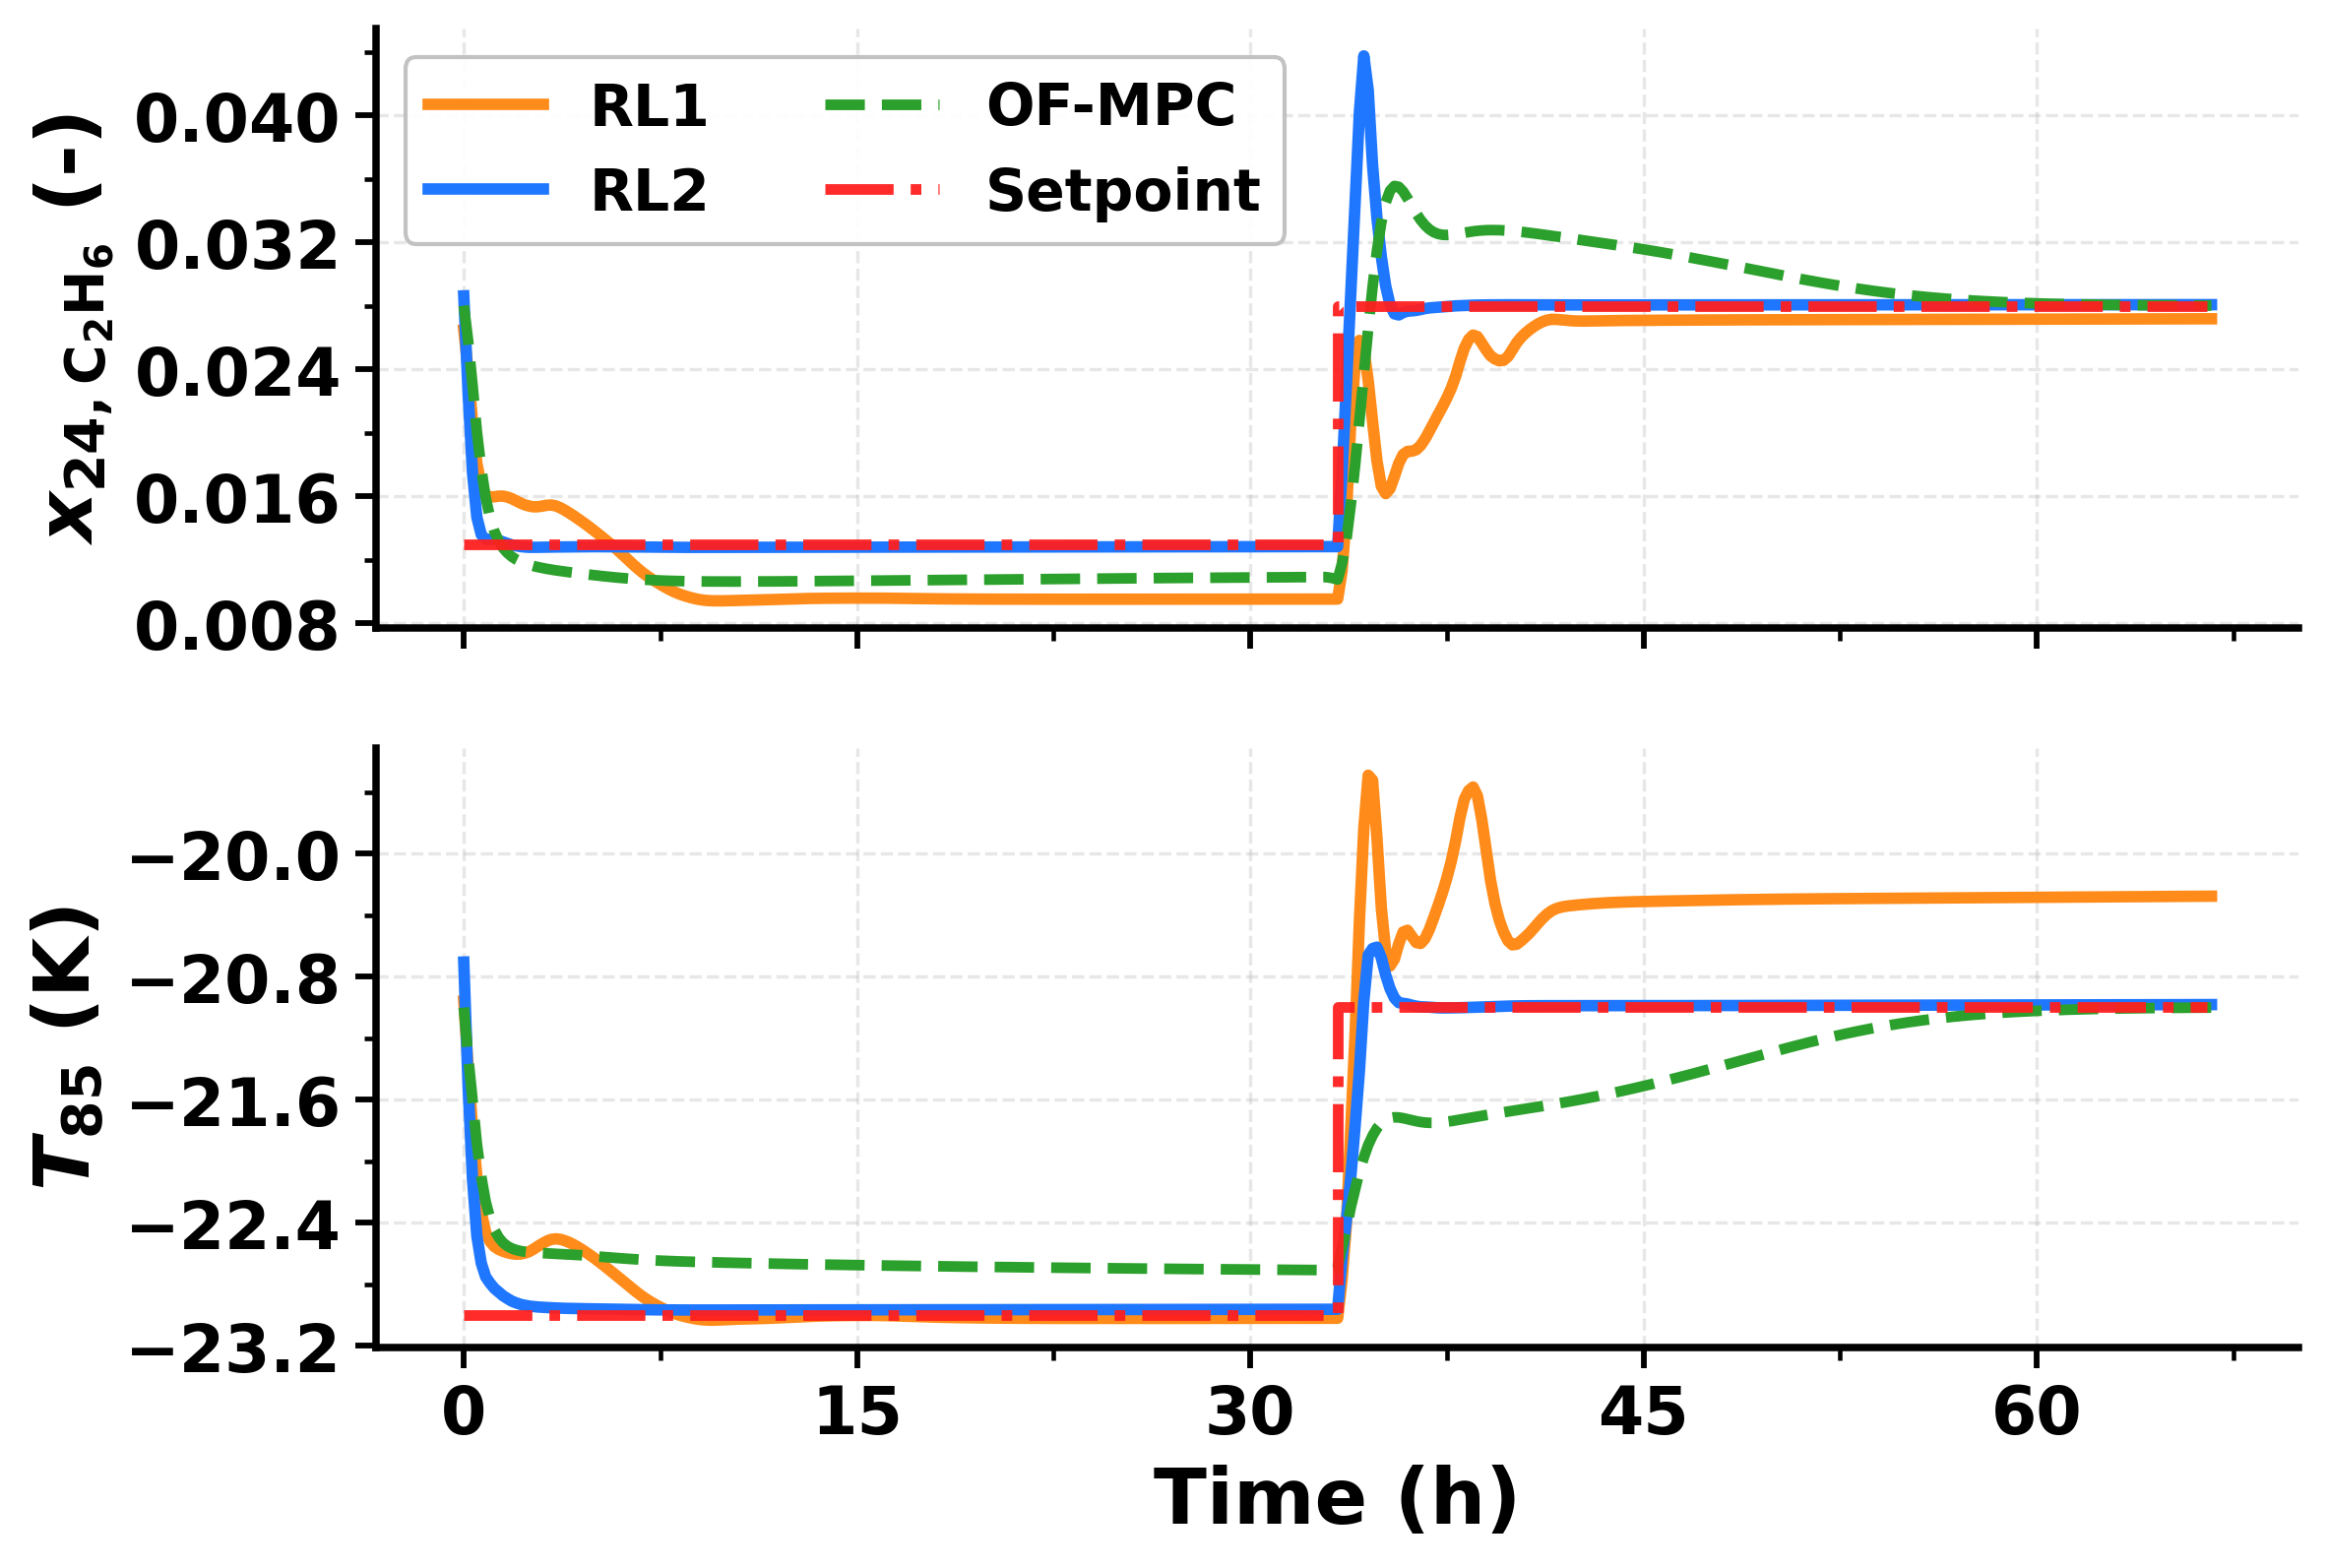
\includegraphics[width=\linewidth,height=0.48\textheight,keepaspectratio]{figures/C2_ramp_outputs_compare_three.png}

\vspace{0.01cm}
{\tiny \textbf{Ramp scenario}}
\end{minipage}
\end{center}

\vspace{0.03cm}

\begin{block}{Cross-scenario message}
\renewcommand{\arraystretch}{1.12}
\begin{tabular}{>{\raggedright\arraybackslash}p{0.27\linewidth} >{\raggedright\arraybackslash}p{0.65\linewidth}}
\textbf{Fluctuation} & RL2 improves disturbance rejection around the operating region. \\
\textbf{Ramp} & RL2 tracks the moving target while keeping the offset advantage. \\
\textbf{Overall} & \(x_{24,\mathrm{C_2H_6}}\) has roughly 90--99\% lower steady-state error than RL1, with substantial improvement in \(T_{85}\).
\end{tabular}
\end{block}

\end{frame}

%============================= Slide 15 ============================
\begin{frame}
\setbeamertemplate{blocks}[default]
\setbeamercolor{block body}{fg=black,bg=lightgray}
\frametitle{\large \textbf{Project 1 takeaway: useful MPC-pretrained RL, but empirical safety}}
\scriptsize
\vspace{-0.36cm}

\begin{columns}[T,onlytextwidth]

\begin{column}{0.55\textwidth}
\centering
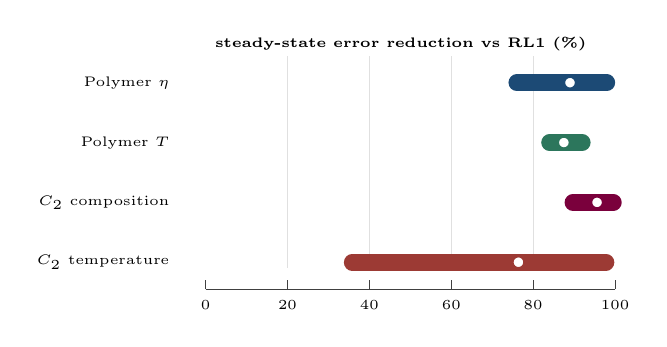
\begin{tikzpicture}[
  x=0.052cm,y=0.76cm,
  every node/.style={font=\tiny}
]
\draw[black!75] (0,-0.45) -- (100,-0.45);
\foreach \x in {0,20,40,60,80,100} {
  \draw[black!75] (\x,-0.45) -- (\x,-0.30);
  \node[anchor=north] at (\x,-0.48) {\x};
}
\foreach \x in {20,40,60,80} {
  \draw[black!12] (\x,-0.1) -- (\x,3.45);
}

\draw[maccblue, line width=6pt, line cap=round] (76,3) -- (98,3);
\filldraw[fill=white, draw=maccblue, line width=1.1pt] (89,3) circle (2.3pt);
\node[anchor=east] at (-6.5,3) {Polymer \(\eta\)};

\draw[maccgreen, line width=6pt, line cap=round] (84,2) -- (92,2);
\filldraw[fill=white, draw=maccgreen, line width=1.1pt] (87.5,2) circle (2.3pt);
\node[anchor=east] at (-6.5,2) {Polymer \(T\)};

\draw[maroon1, line width=6pt, line cap=round] (89.7,1) -- (99.6,1);
\filldraw[fill=white, draw=maroon1, line width=1.1pt] (95.6,1) circle (2.3pt);
\node[anchor=east] at (-6.5,1) {\(C_2\) composition};

\draw[maccred, line width=6pt, line cap=round] (35.8,0) -- (97.8,0);
\filldraw[fill=white, draw=maccred, line width=1.1pt] (76.4,0) circle (2.3pt);
\node[anchor=east] at (-6.5,0) {\(C_2\) temperature};

\node[anchor=west] at (0,3.65) {\textbf{steady-state error reduction vs RL1 (\%)}};
\end{tikzpicture}

\vspace{0.03cm}
{\tiny \textbf{Figure:} min-to-max range across reported setpoints and scenarios. White marker shows the mean.}

\vspace{0.01cm}
\begin{block}{Publication}
\justifying
Published in \textit{Industrial \& Engineering Chemistry Research (I\&ECR)}.
\end{block}
\end{column}

\begin{column}{0.42\textwidth}

\begin{block}{Established}
\begin{itemize}\justifying
  \setlength{\itemsep}{0.12em}
  \item MPC pretraining avoids random online initialization.
  \item RL2 improves final offset without changing the plant-side architecture.
  \item The improvement transfers from polymer to the Aspen \(C_2\) case.
\end{itemize}
\end{block}

\vspace{0.02cm}

\begin{block}{Still empirical}
\begin{itemize}\justifying
  \setlength{\itemsep}{0.12em}
  \item Safety is observed in simulation, not certified before each move.
  \item This motivates keeping MPC more explicitly in the loop.
\end{itemize}
\end{block}

\end{column}

\end{columns}

{\centering
\begin{beamercolorbox}[wd=0.94\textwidth,sep=1.5pt,center,rounded=true]{takeawaybox}
\textbf{\textcolor{maroon1}{Takeaway:}} Project 1 shows practical benefits, but the next step is to make learning more structured and safety-aware.
\end{beamercolorbox}
\par}

\end{frame}

%============================= Slide 16 ============================
\begin{frame}
\setbeamertemplate{blocks}[default]
\setbeamercolor{block body}{fg=black,bg=lightgray}
\frametitle{\large \textbf{Project 2: RL supervises MPC instead of replacing it}}
\scriptsize
\vspace{-0.30cm}

\begin{columns}[T,onlytextwidth]

\begin{column}{0.44\textwidth}

\begin{block}{Core idea}
\begin{itemize}\justifying
  \setlength{\itemsep}{0.35ex}
  \item Project 2 keeps the same offset-free MPC backbone from Project 1.
  \item RL does not become the low-level controller; it only chooses supervisory MPC parameters online.
  \item The plant still receives the first move from the MPC optimizer, so constraints and receding-horizon structure stay intact.
  \item The learned supervisory variable can be the horizon, model, penalties, residual correction, or later a combined action.
\end{itemize}
\end{block}

\vspace{0.02cm}

\begin{block}{What is intentionally reused}
\begin{itemize}\justifying
  \setlength{\itemsep}{0.35ex}
  \item The replay-buffer workflow is the same off-policy transition storage used in Project 1.
  \item The reward function is also the same Project 1 shaped reward, so the comparison isolates \emph{what MPC knob is adapted}.
  \item The question is therefore structural: which supervisory degree of freedom is most useful to learn around MPC?
\end{itemize}
\end{block}

\end{column}

\begin{column}{0.53\textwidth}
\centering
\vspace{0.15cm}

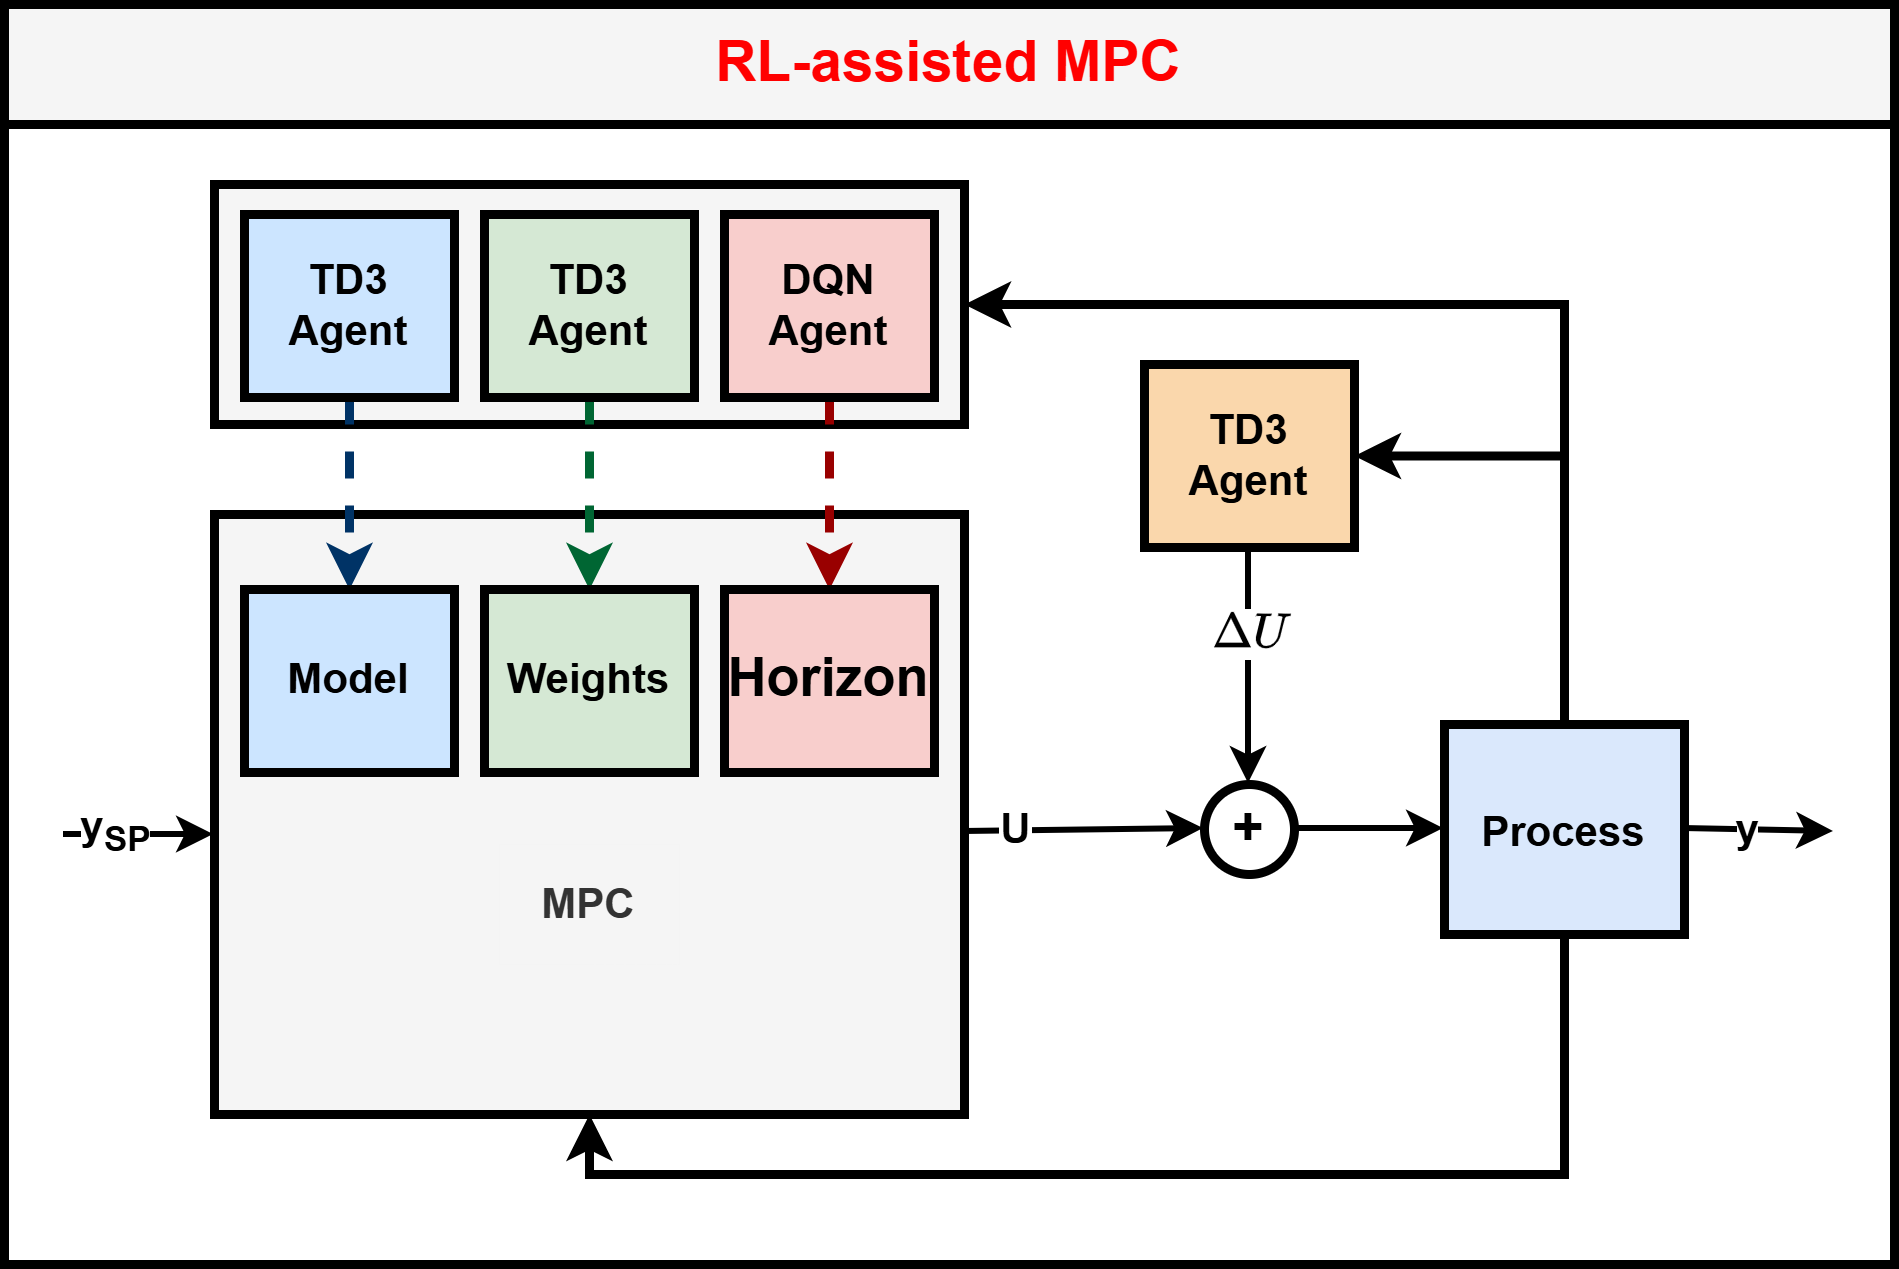
\includegraphics[
  width=\linewidth,
  height=0.60\textheight,
  keepaspectratio,
  trim=6 4 6 4,
  clip
]{figures/RLAssistedDiagram.png}

\vspace{0.02cm}
{\tiny \textbf{Figure:} the policy updates supervisory MPC parameters while the optimizer still computes the applied move.}

\end{column}

\end{columns}

\takeawaybox{Project 2 asks which MPC design variable should adapt online, while keeping the same MPC backbone, replay structure, and reward used in Project 1.}

\end{frame}

%============================= Slide 17 ============================
\begin{frame}
\setbeamertemplate{blocks}[default]
\setbeamercolor{block body}{fg=black,bg=lightgray}
\frametitle{\large \textbf{Project 2 method: shared state, shared reward, different supervisory actions}}
\scriptsize
\vspace{-0.32cm}

\begin{columns}[T,onlytextwidth]

\begin{column}{0.49\textwidth}

\begin{block}{Shared RL state and reward}
\justifying
\[
\begin{aligned}
\bar{s}_k &= \big[\hat{x}^{aug}_k,\; y_k^{sp},\; u_{k-1}\big], \\
s_k &= 
\begin{cases}
\bar{s}_k, & \text{standard state},\\
\big[\bar{s}_k,\nu_k,\varepsilon_k,\rho_k\big], & \text{mismatch state},
\end{cases} \\
\nu_k &= T\!\left(\dfrac{y_k-\hat{y}_k}{\sigma_\nu}\right), \qquad
\varepsilon_k = T\!\left(\dfrac{y_k-y_k^{sp}}{\sigma_\varepsilon}\right).
\end{aligned}
\]
\[
r_k = r_{\mathrm{Proj1}}(e_k,\Delta u_k,y_k^{sp}),
\]
with the same Project 1 shaped reward and the same replay tuple
\[
\big(s_k,a_k,r_k,s_{k+1}\big).
\]
\end{block}

\vspace{0.02cm}

\begin{block}{Supervisory action map}
\justifying
\[
\begin{aligned}
\text{Horizon:}\quad & a_k \in \mathcal{H}, \qquad \theta_k=(N_{p,k},N_{c,k}), \\
\text{Matrix:}\quad & a_k \mapsto (\alpha_k,\beta_{1,k},\beta_{2,k}), \\
& A_k=\alpha_k A_0,\;\; B_k=B_0\,\mathrm{diag}(\beta_{1,k},\beta_{2,k}), \\
\text{Weights:}\quad & a_k \mapsto (\lambda_{Q1,k},\lambda_{Q2,k},\lambda_{R1,k},\lambda_{R2,k}), \\
& Q_k=\mathrm{diag}(\lambda_{Q1,k},\lambda_{Q2,k})Q_0,\;\;
R_k=\mathrm{diag}(\lambda_{R1,k},\lambda_{R2,k})R_0, \\
\text{Residual:}\quad & a_k \mapsto \Delta u_k^{res}, \qquad
u_k=\mathrm{sat}\!\left(u_k^{MPC}+\rho_k\Delta u_k^{res}\right).
\end{aligned}
\]
\end{block}

\end{column}

\begin{column}{0.49\textwidth}

\begin{block}{Shared rollout algorithm}
\begin{enumerate}\justifying
  \setlength{\itemsep}{0.25ex}
  \item Update the observer and build \(s_k\) from the augmented estimate, setpoint, previous input, and mismatch features if enabled.
  \item During warm start use the nominal supervisory action; afterwards evaluate the RL policy every decision interval.
  \item Map the policy output into \(\theta_k\): horizons, model multipliers, weight multipliers, or residual correction.
  \item Solve MPC with \(\theta_k\) and apply only the first move; for the residual method, correct that move before plant actuation.
  \item Compute \(r_k\), append \((s_k,a_k,r_k,s_{k+1})\) to replay, and update the off-policy agent.
\end{enumerate}
\end{block}

\vspace{0.02cm}

\begin{block}{Code path used for this slide}
\begin{itemize}\justifying
  \setlength{\itemsep}{0.25ex}
  \item State construction: \texttt{utils/state\_features.py}
  \item Reward construction: \texttt{utils/rewards.py}
  \item Shared push/train logic: \texttt{utils/agent\_step\_runtime.py}
  \item Method runners: \texttt{horizon\_runner\_dueling.py}, \texttt{matrix\_runner.py}, \texttt{weights\_runner.py}, \texttt{residual\_runner.py}
\end{itemize}
\end{block}

\end{column}

\end{columns}

\takeawaybox{All Project 2 agents share the same state, reward, replay, and MPC backbone; only the action-to-parameter map changes from one supervisory method to another.}

\end{frame}

%============================= Slide 18 ============================
\begin{frame}
\setbeamertemplate{blocks}[default]
\setbeamercolor{block body}{fg=black,bg=lightgray}
\frametitle{\large \textbf{Horizon Agent: RL chooses the prediction horizon instead of fixed look-ahead}}
\scriptsize
\vspace{-0.32cm}

\begin{columns}[T,onlytextwidth]

\begin{column}{0.39\textwidth}
\begin{block}{Method}
\justifying
The horizon agent uses dueling DQN because the supervisory action is discrete:
\[
a_k \in \mathcal{H}=\{(N_p,N_c)^{(1)},\ldots,(N_p,N_c)^{(m)}\}.
\]
The network estimates
\[
Q(s_k,a)=V(s_k)+A(s_k,a)-\frac{1}{|\mathcal{H}|}\sum_{a'}A(s_k,a'),
\]
then MPC solves with the selected \((N_p,N_c)\).
\end{block}

\vspace{0.02cm}

\begin{block}{Interpretation}
\begin{itemize}\justifying
  \setlength{\itemsep}{0.20ex}
  \item Shorter horizons react faster when the state is near a disturbance or setpoint switch.
  \item Longer horizons preserve anticipation when the process is close to nominal.
  \item This agent changes optimization look-ahead without touching the model or plant input map.
\end{itemize}
\end{block}

\vspace{0.02cm}

\begin{block}{Latest polymer result}
\justifying
Current multiseed mean:
\[
\bar{R}_{\mathrm{final}}=-2.60\pm 0.05,\quad
\overline{\mathrm{RMSE}}=0.293\pm 0.001.
\]
Against baseline MPC, the mean RMSE drops by \(0.087\) and the mean IAE drops to \(7499.8\).
\end{block}
\end{column}

\begin{column}{0.58\textwidth}
\centering
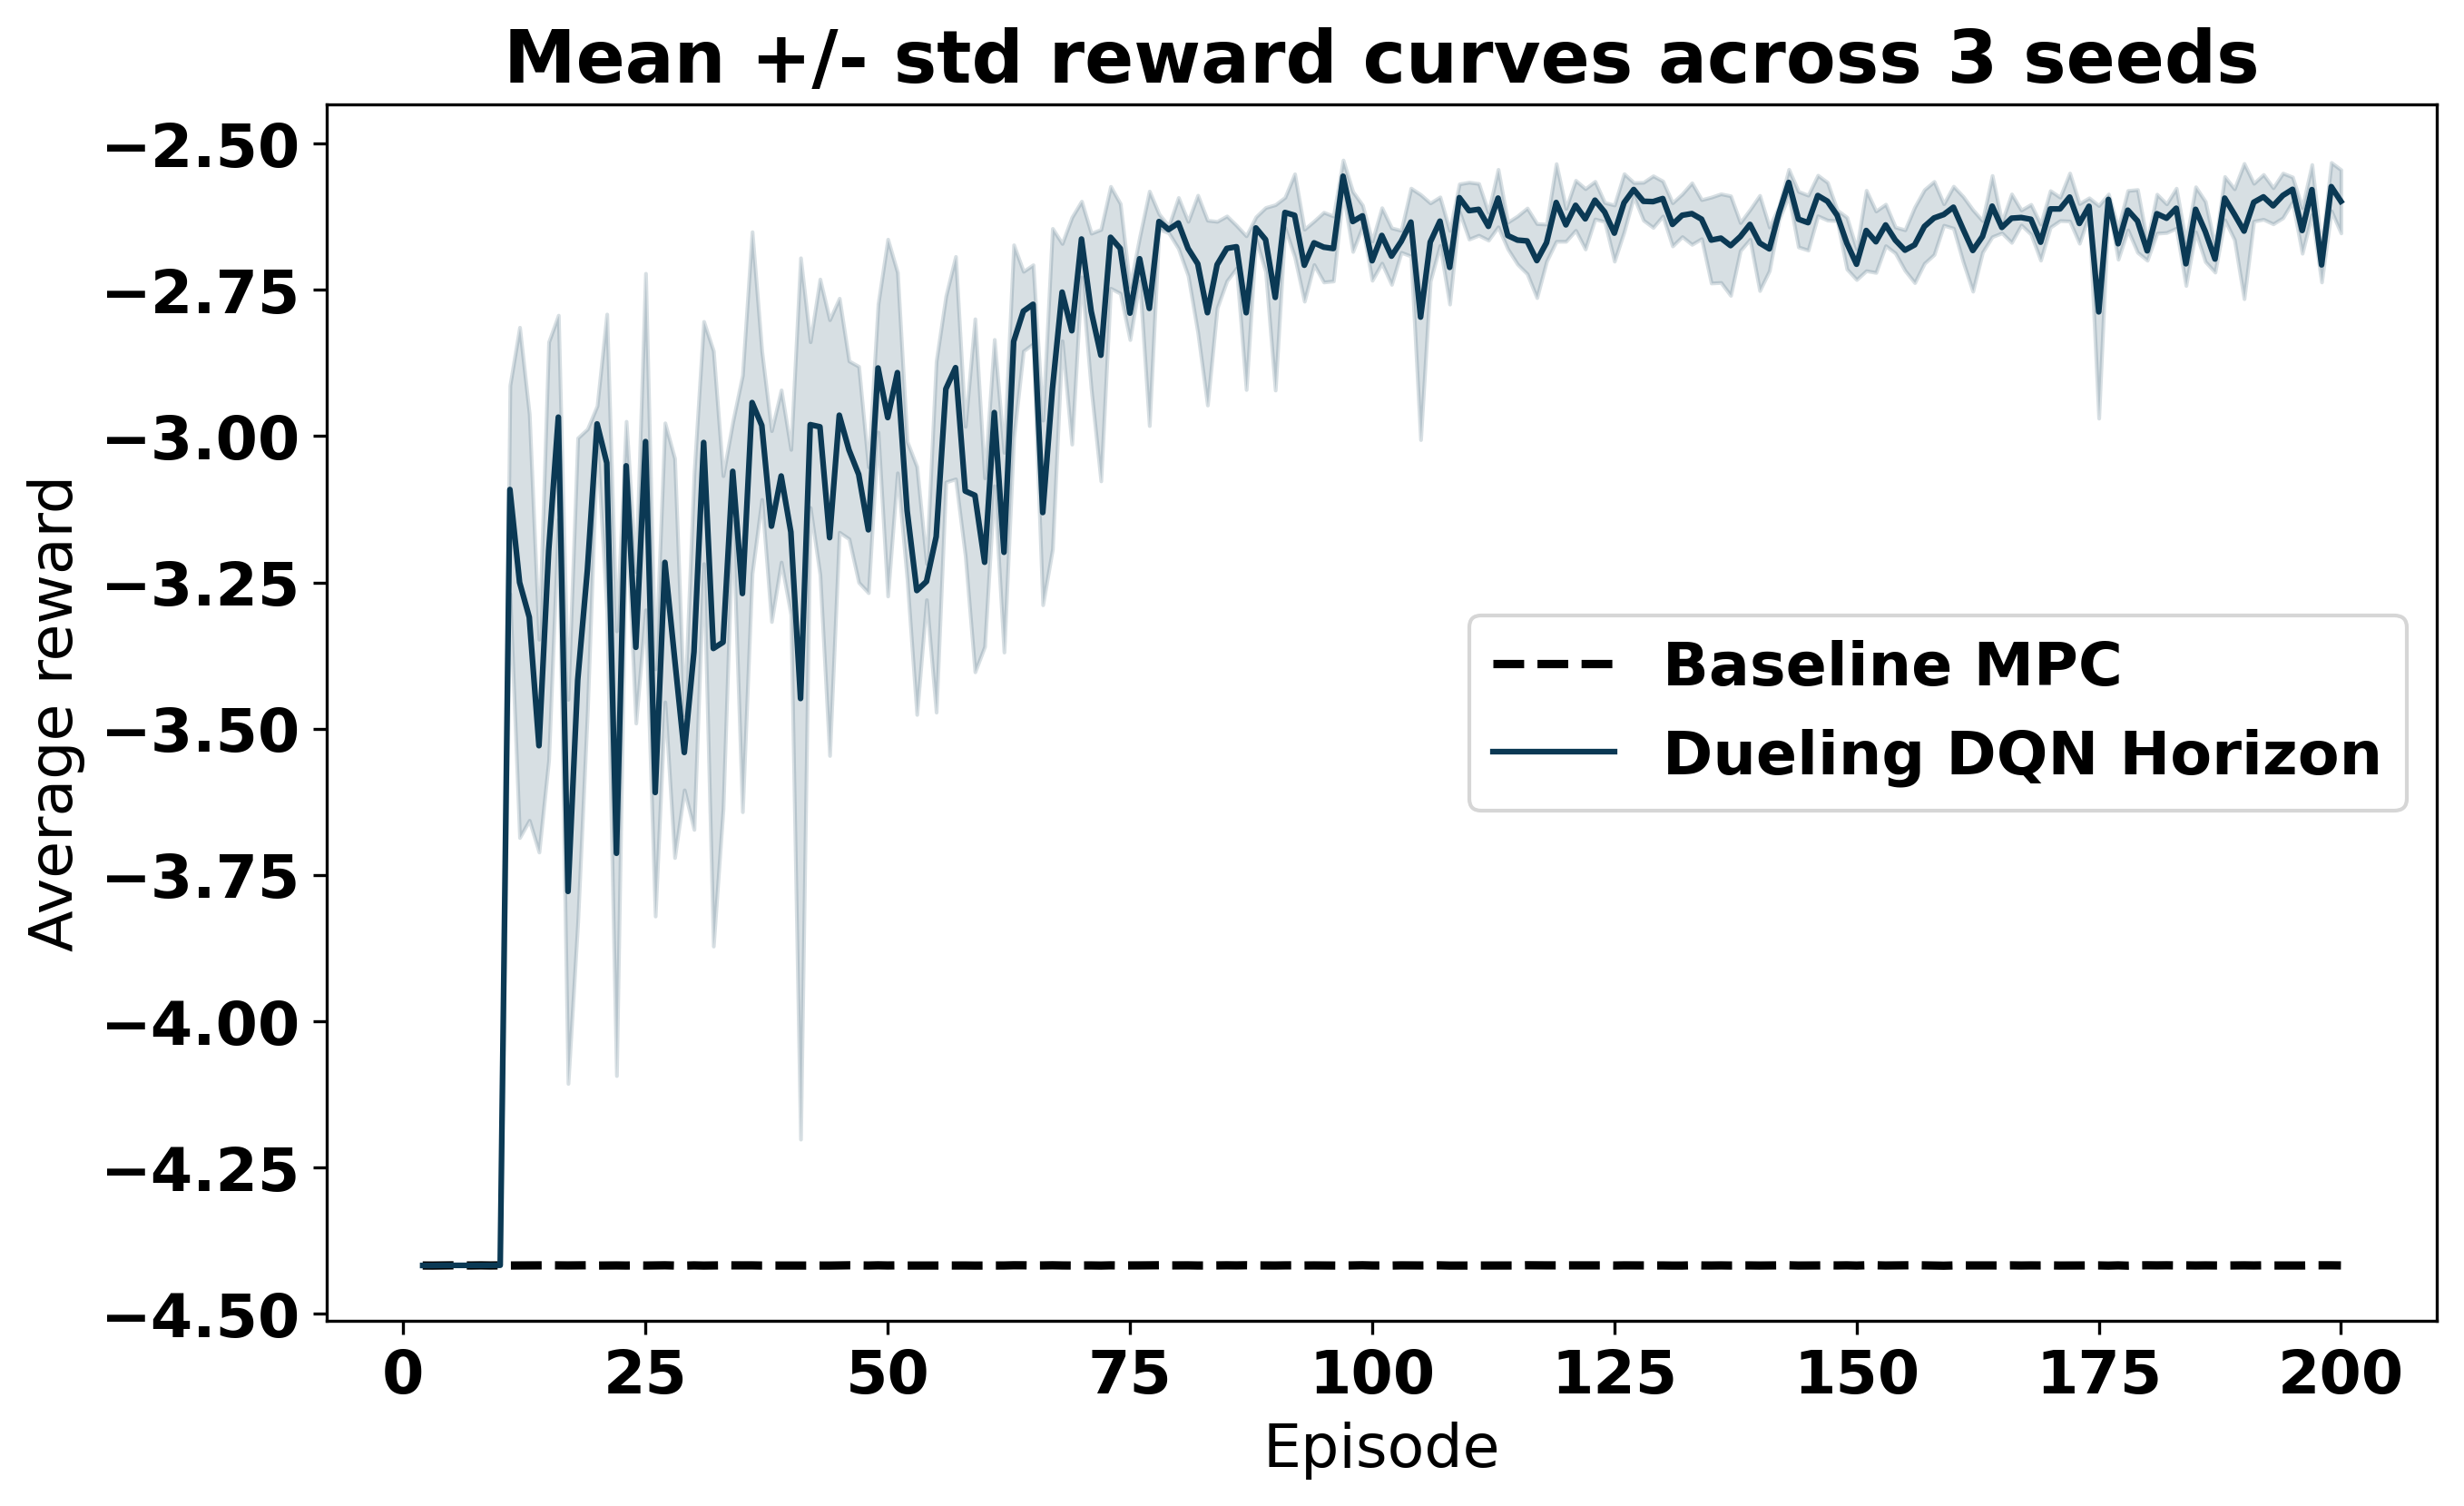
\includegraphics[
  width=\linewidth,
  height=0.20\textheight,
  keepaspectratio,
  trim=10 10 10 10,
  clip
]{figures/polymer_horizon_reward.png}

\vspace{0.01cm}
{\tiny \textbf{Reward across seeds:} the horizon policy learns steadily and finishes well above the fixed-MPC reward line.}

\vspace{0.02cm}
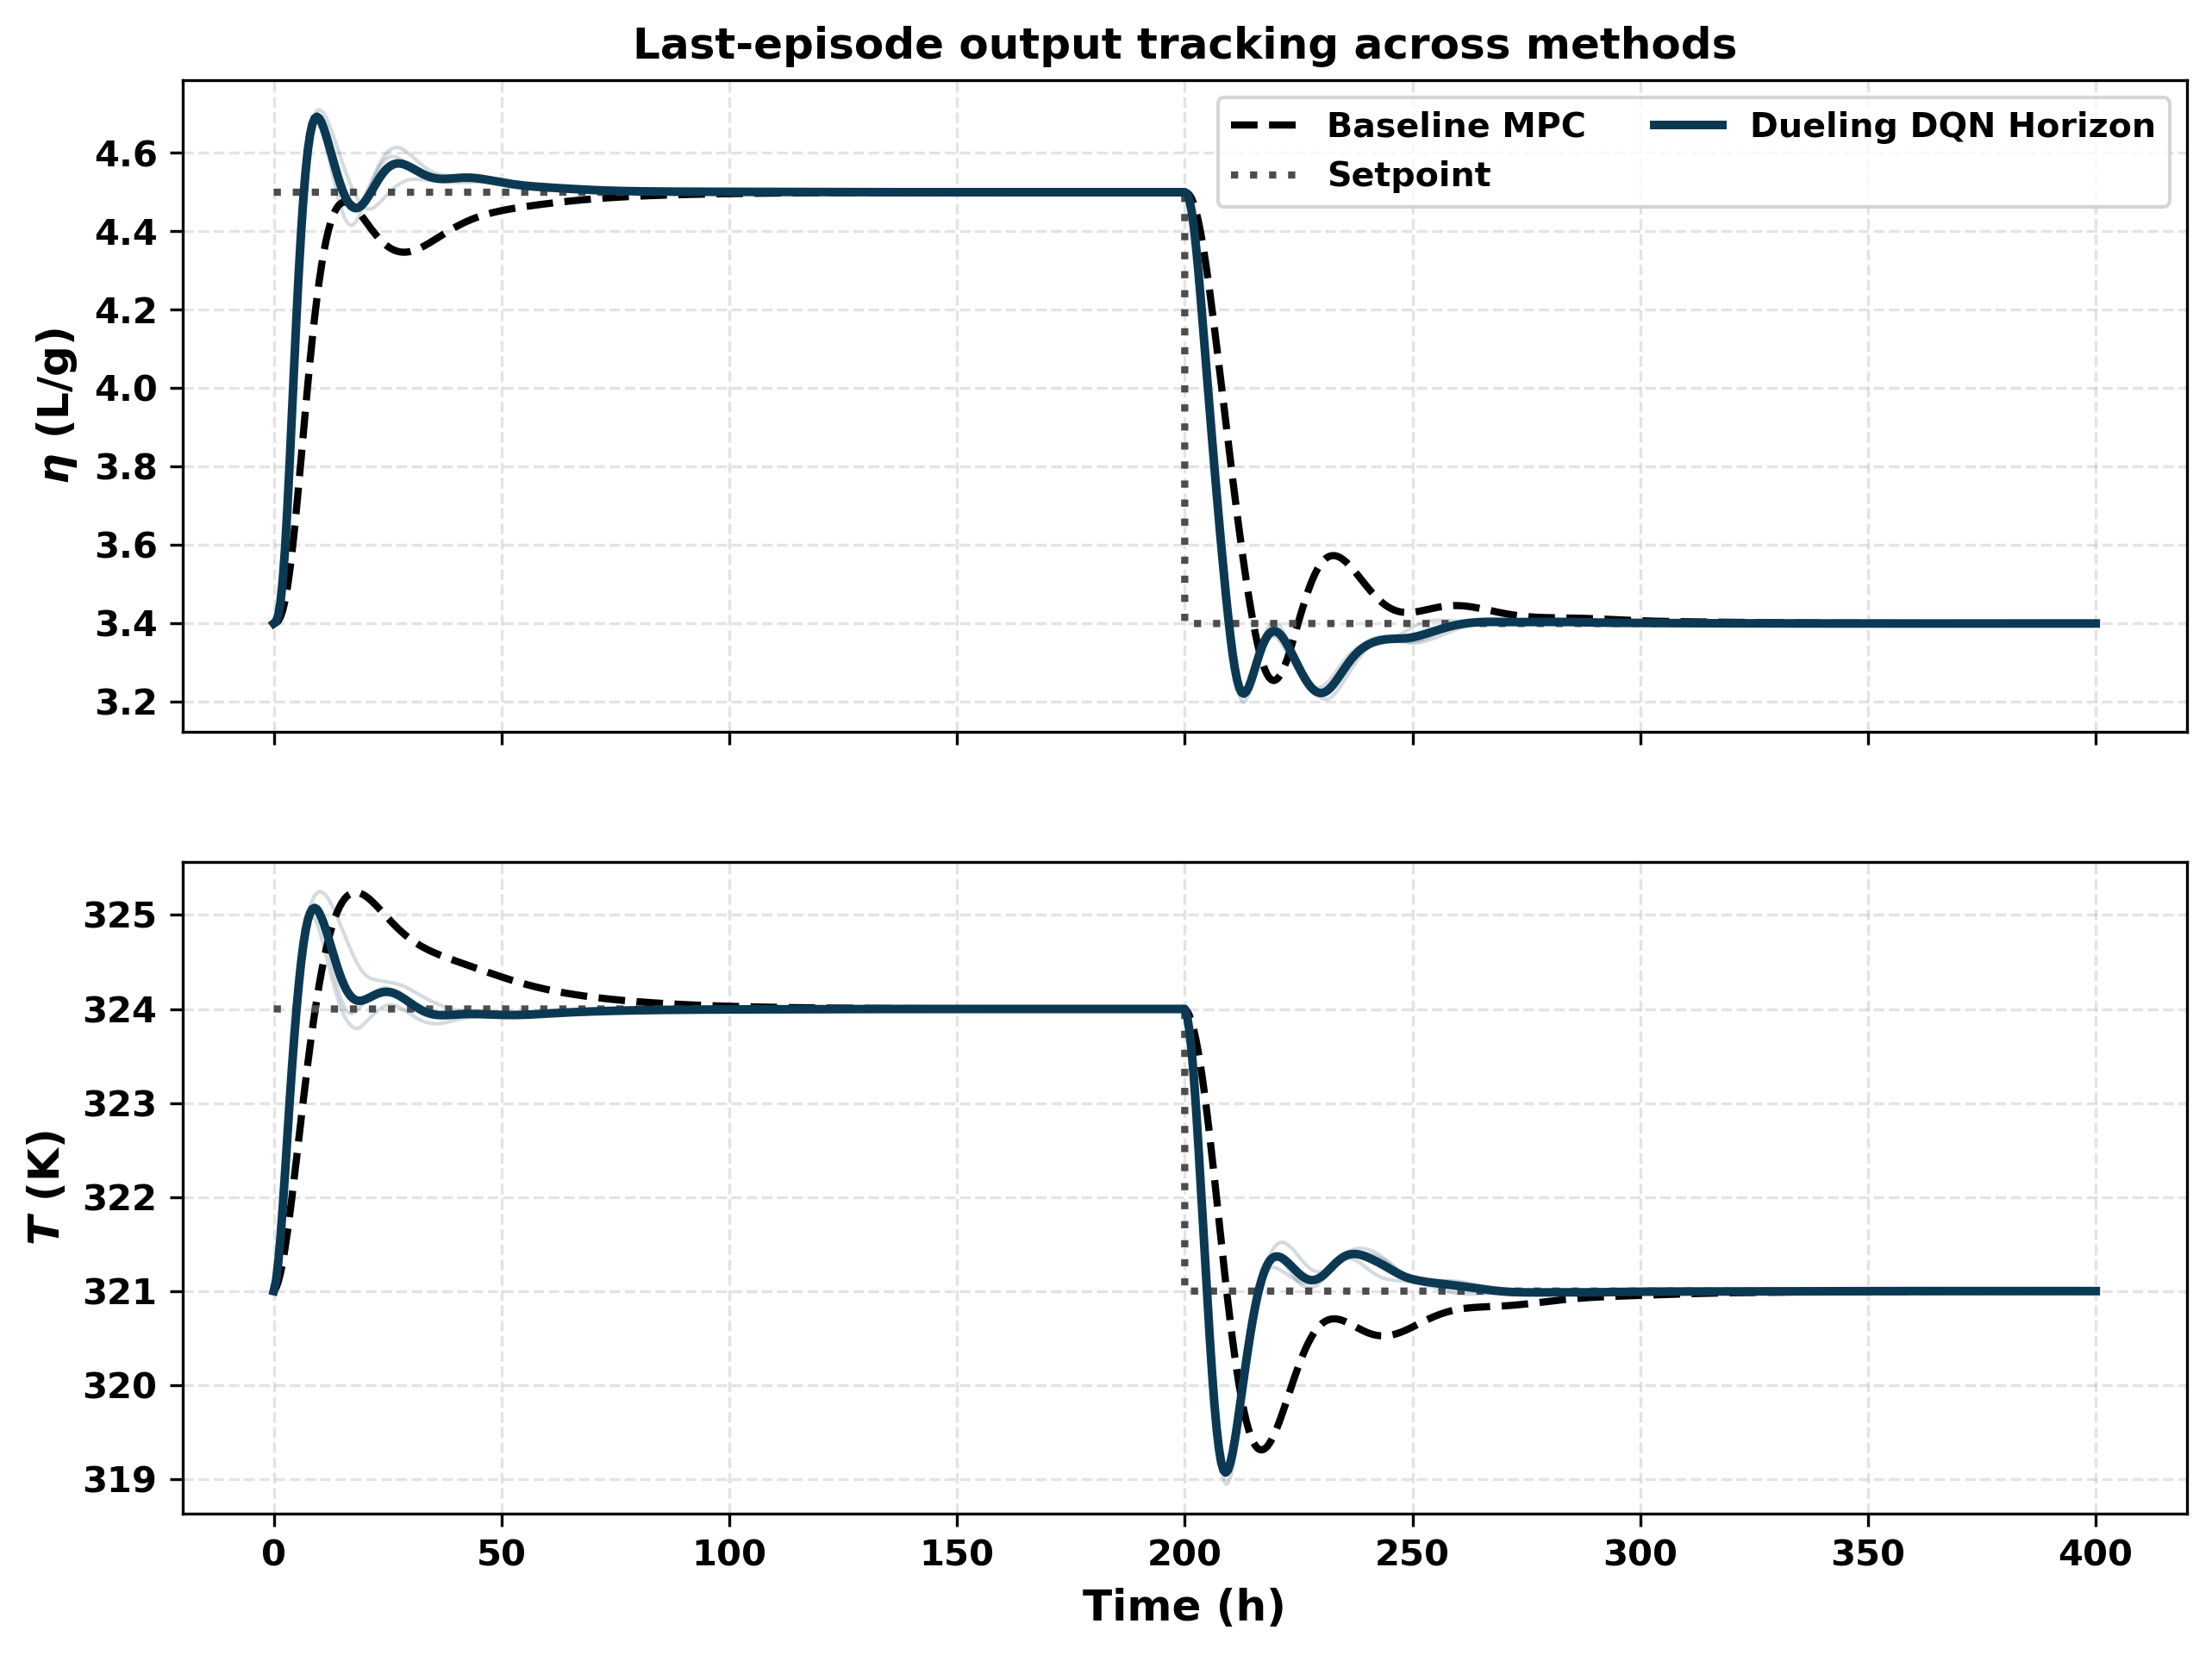
\includegraphics[
  width=\linewidth,
  height=0.31\textheight,
  keepaspectratio,
  trim=10 10 10 10,
  clip
]{figures/polymer_horizon_last_episode.png}

\vspace{0.01cm}
{\tiny \textbf{Last-episode evaluation:} both viscosity and temperature settle closer to the setpoint with smaller late oscillation than fixed MPC.}
\end{column}

\end{columns}

\takeawaybox{Adaptive horizon selection is the strongest current single-agent polymer result in both reward and tracking metrics.}

\end{frame}

%============================= Slide 19 ============================
\begin{frame}
\setbeamertemplate{blocks}[default]
\setbeamercolor{block body}{fg=black,bg=lightgray}
\frametitle{\large \textbf{Matrix Agent: RL perturbs the internal MPC model used for prediction}}
\scriptsize
\vspace{-0.32cm}

\begin{columns}[T,onlytextwidth]

\begin{column}{0.39\textwidth}
\begin{block}{Method}
\justifying
The matrix agent keeps the optimizer fixed but changes the linear prediction model:
\[
A_k=\alpha_k A_0,\qquad
B_k=B_0\operatorname{diag}(\beta_{1,k},\beta_{2,k}).
\]
TD3 outputs a continuous action \(a_k=[\alpha_k,\beta_{1,k},\beta_{2,k}]^\top\), and MPC computes the move using \((A_k,B_k)\).
\end{block}

\vspace{0.02cm}

\begin{block}{Interpretation}
\begin{itemize}\justifying
  \setlength{\itemsep}{0.20ex}
  \item \(\alpha_k\) changes the effective process memory and speed.
  \item \(\beta_{i,k}\) change the predicted input gains seen by MPC.
  \item This is powerful when model mismatch dominates, but it is also the easiest supervisory family to overtune.
\end{itemize}
\end{block}

\vspace{0.02cm}

\begin{block}{Latest polymer result}
\justifying
Current multiseed mean:
\[
\bar{R}_{\mathrm{final}}=-3.63\pm 0.04,\quad
\overline{\mathrm{RMSE}}=0.374\pm 0.003.
\]
That is only a small RMSE improvement over baseline MPC, and the mean IAE rises to \(13721.5\).
\end{block}
\end{column}

\begin{column}{0.58\textwidth}
\centering
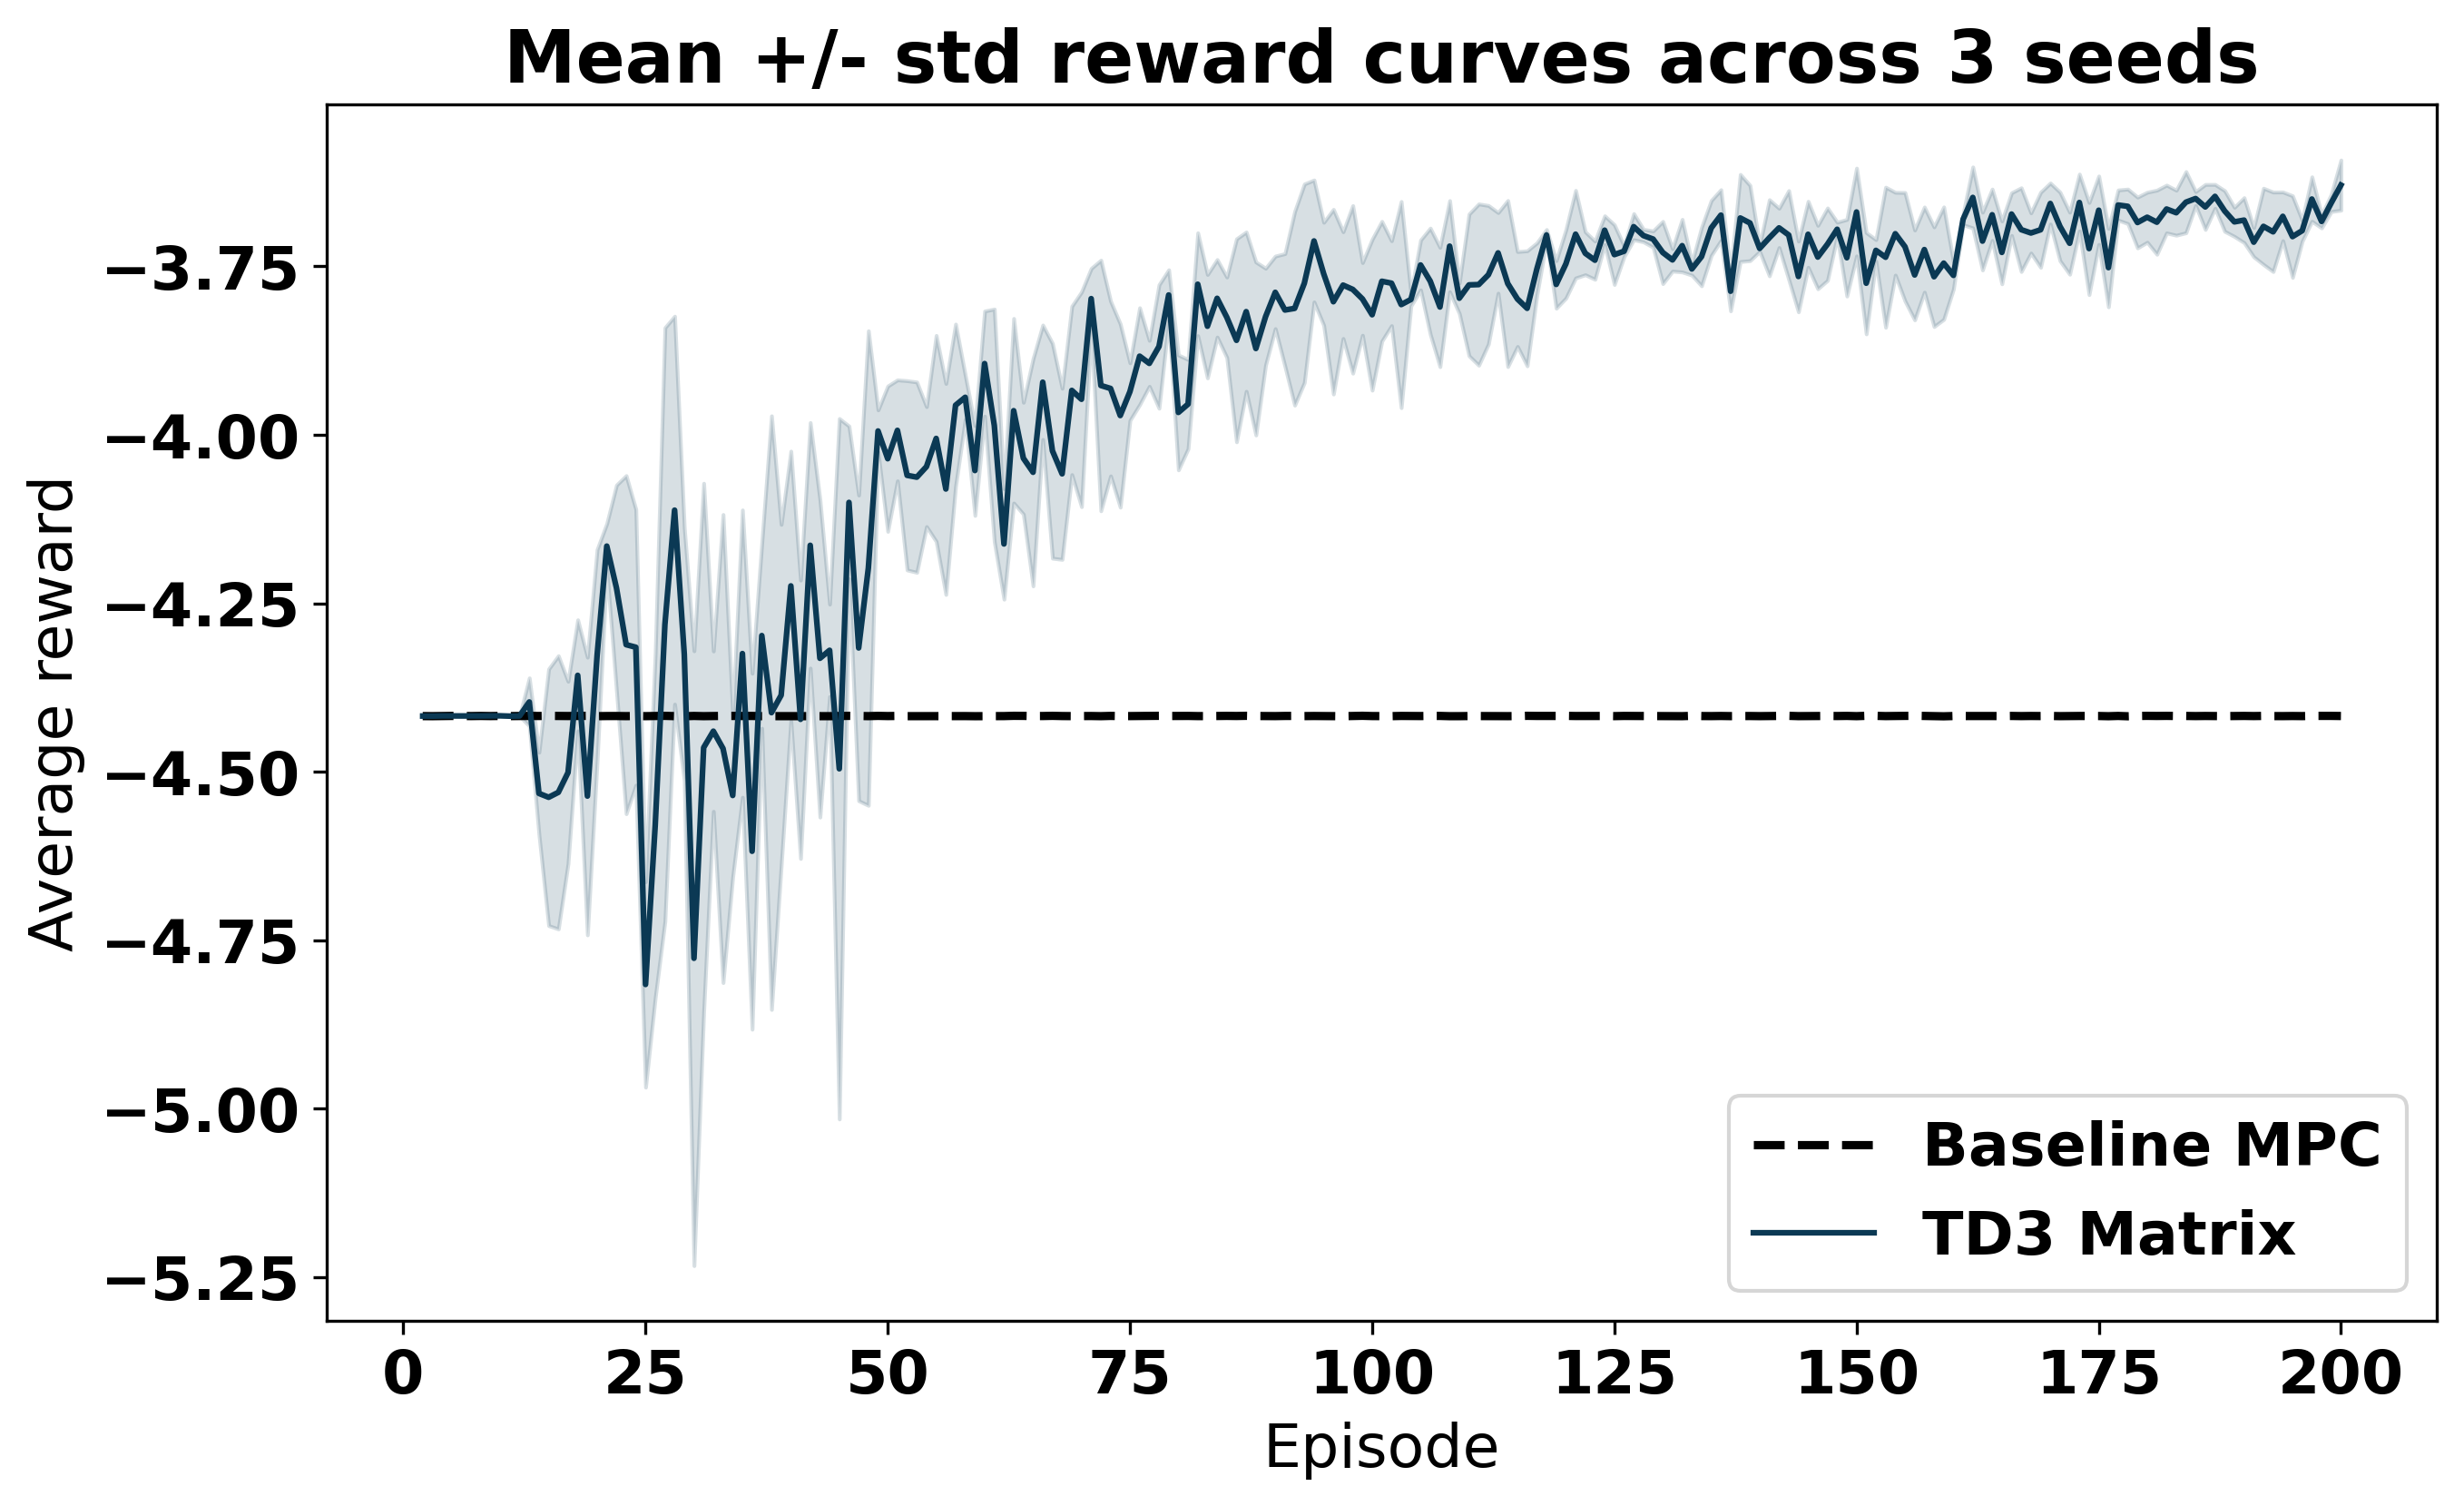
\includegraphics[
  width=\linewidth,
  height=0.20\textheight,
  keepaspectratio,
  trim=10 10 10 10,
  clip
]{figures/polymer_matrix_reward.png}

\vspace{0.01cm}
{\tiny \textbf{Reward across seeds:} learning improves from the early unstable region, but the converged reward remains far below the horizon and weight agents.}

\vspace{0.02cm}
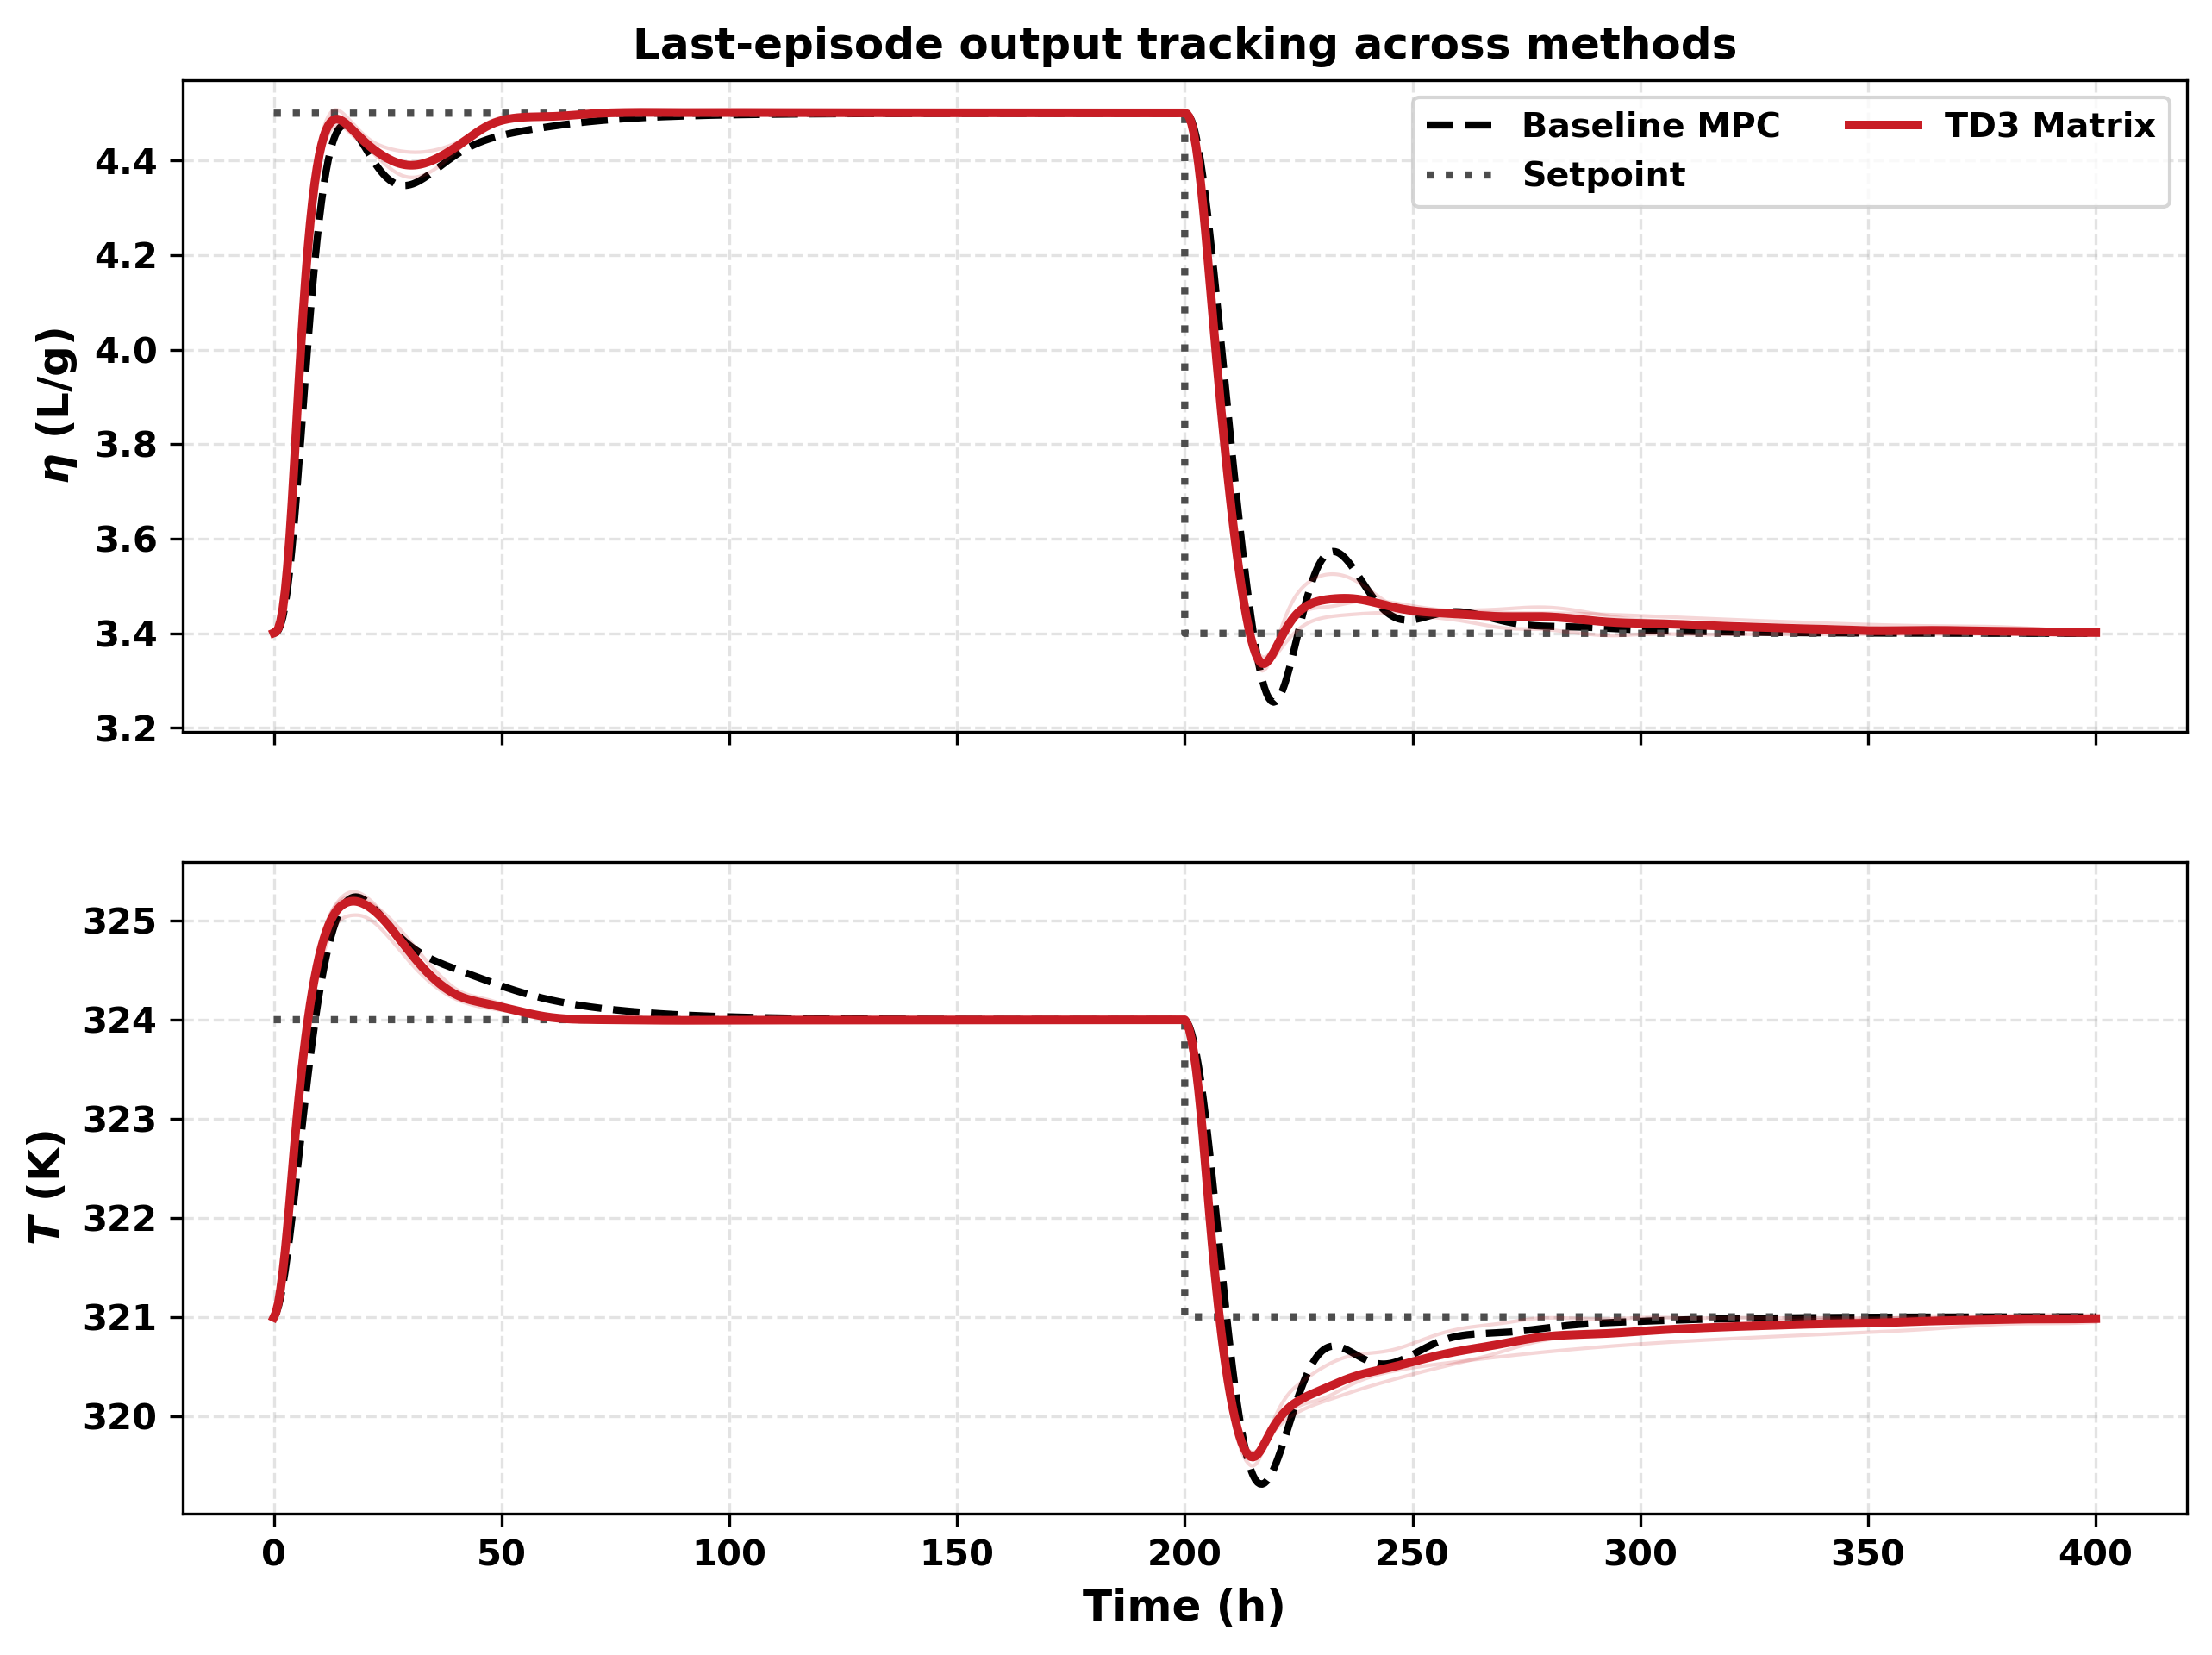
\includegraphics[
  width=\linewidth,
  height=0.31\textheight,
  keepaspectratio,
  trim=10 10 10 10,
  clip
]{figures/polymer_matrix_last_episode.png}

\vspace{0.01cm}
{\tiny \textbf{Last-episode evaluation:} the matrix agent matches the main setpoint transitions reasonably well, but the aggregate advantage over baseline is limited in this run.}
\end{column}

\end{columns}

\takeawaybox{Model adaptation is interpretable and promising, but the latest polymer run shows it is not yet the most reliable supervisory knob.}

\end{frame}

%============================= Slide 20 ============================
\begin{frame}
\setbeamertemplate{blocks}[default]
\setbeamercolor{block body}{fg=black,bg=lightgray}
\frametitle{\large \textbf{Weight Agent: RL retunes the MPC cost to trade off speed and smoothness online}}
\scriptsize
\vspace{-0.32cm}

\begin{columns}[T,onlytextwidth]

\begin{column}{0.39\textwidth}
\begin{block}{Method}
\justifying
The weight agent leaves the model fixed and changes the objective:
\[
J_k=\sum_{i=1}^{N_p}\|y_{k+i}-y_{k+i}^{sp}\|_{Q_k}^2
+\sum_{i=0}^{N_c-1}\|\Delta u_{k+i}\|_{R_k}^2.
\]
TD3 outputs positive multipliers such that
\[
Q_k=\operatorname{diag}(q_k)Q_0,\qquad
R_k=\operatorname{diag}(r_k)R_0.
\]
\end{block}

\vspace{0.02cm}

\begin{block}{Interpretation}
\begin{itemize}\justifying
  \setlength{\itemsep}{0.20ex}
  \item Larger \(q_k\) make MPC chase output error more aggressively.
  \item Larger \(r_k\) penalize input movement and produce smoother actions.
  \item Because the prediction model stays nominal, this is the safest adaptive family to interpret physically.
\end{itemize}
\end{block}

\vspace{0.02cm}

\begin{block}{Latest polymer result}
\justifying
Current multiseed mean:
\[
\bar{R}_{\mathrm{final}}=-2.77\pm 0.06,\quad
\overline{\mathrm{RMSE}}=0.334\pm 0.007.
\]
The mean IAE drops to \(10231.9\), making this the second-best current single-agent result after horizon adaptation.
\end{block}
\end{column}

\begin{column}{0.58\textwidth}
\centering
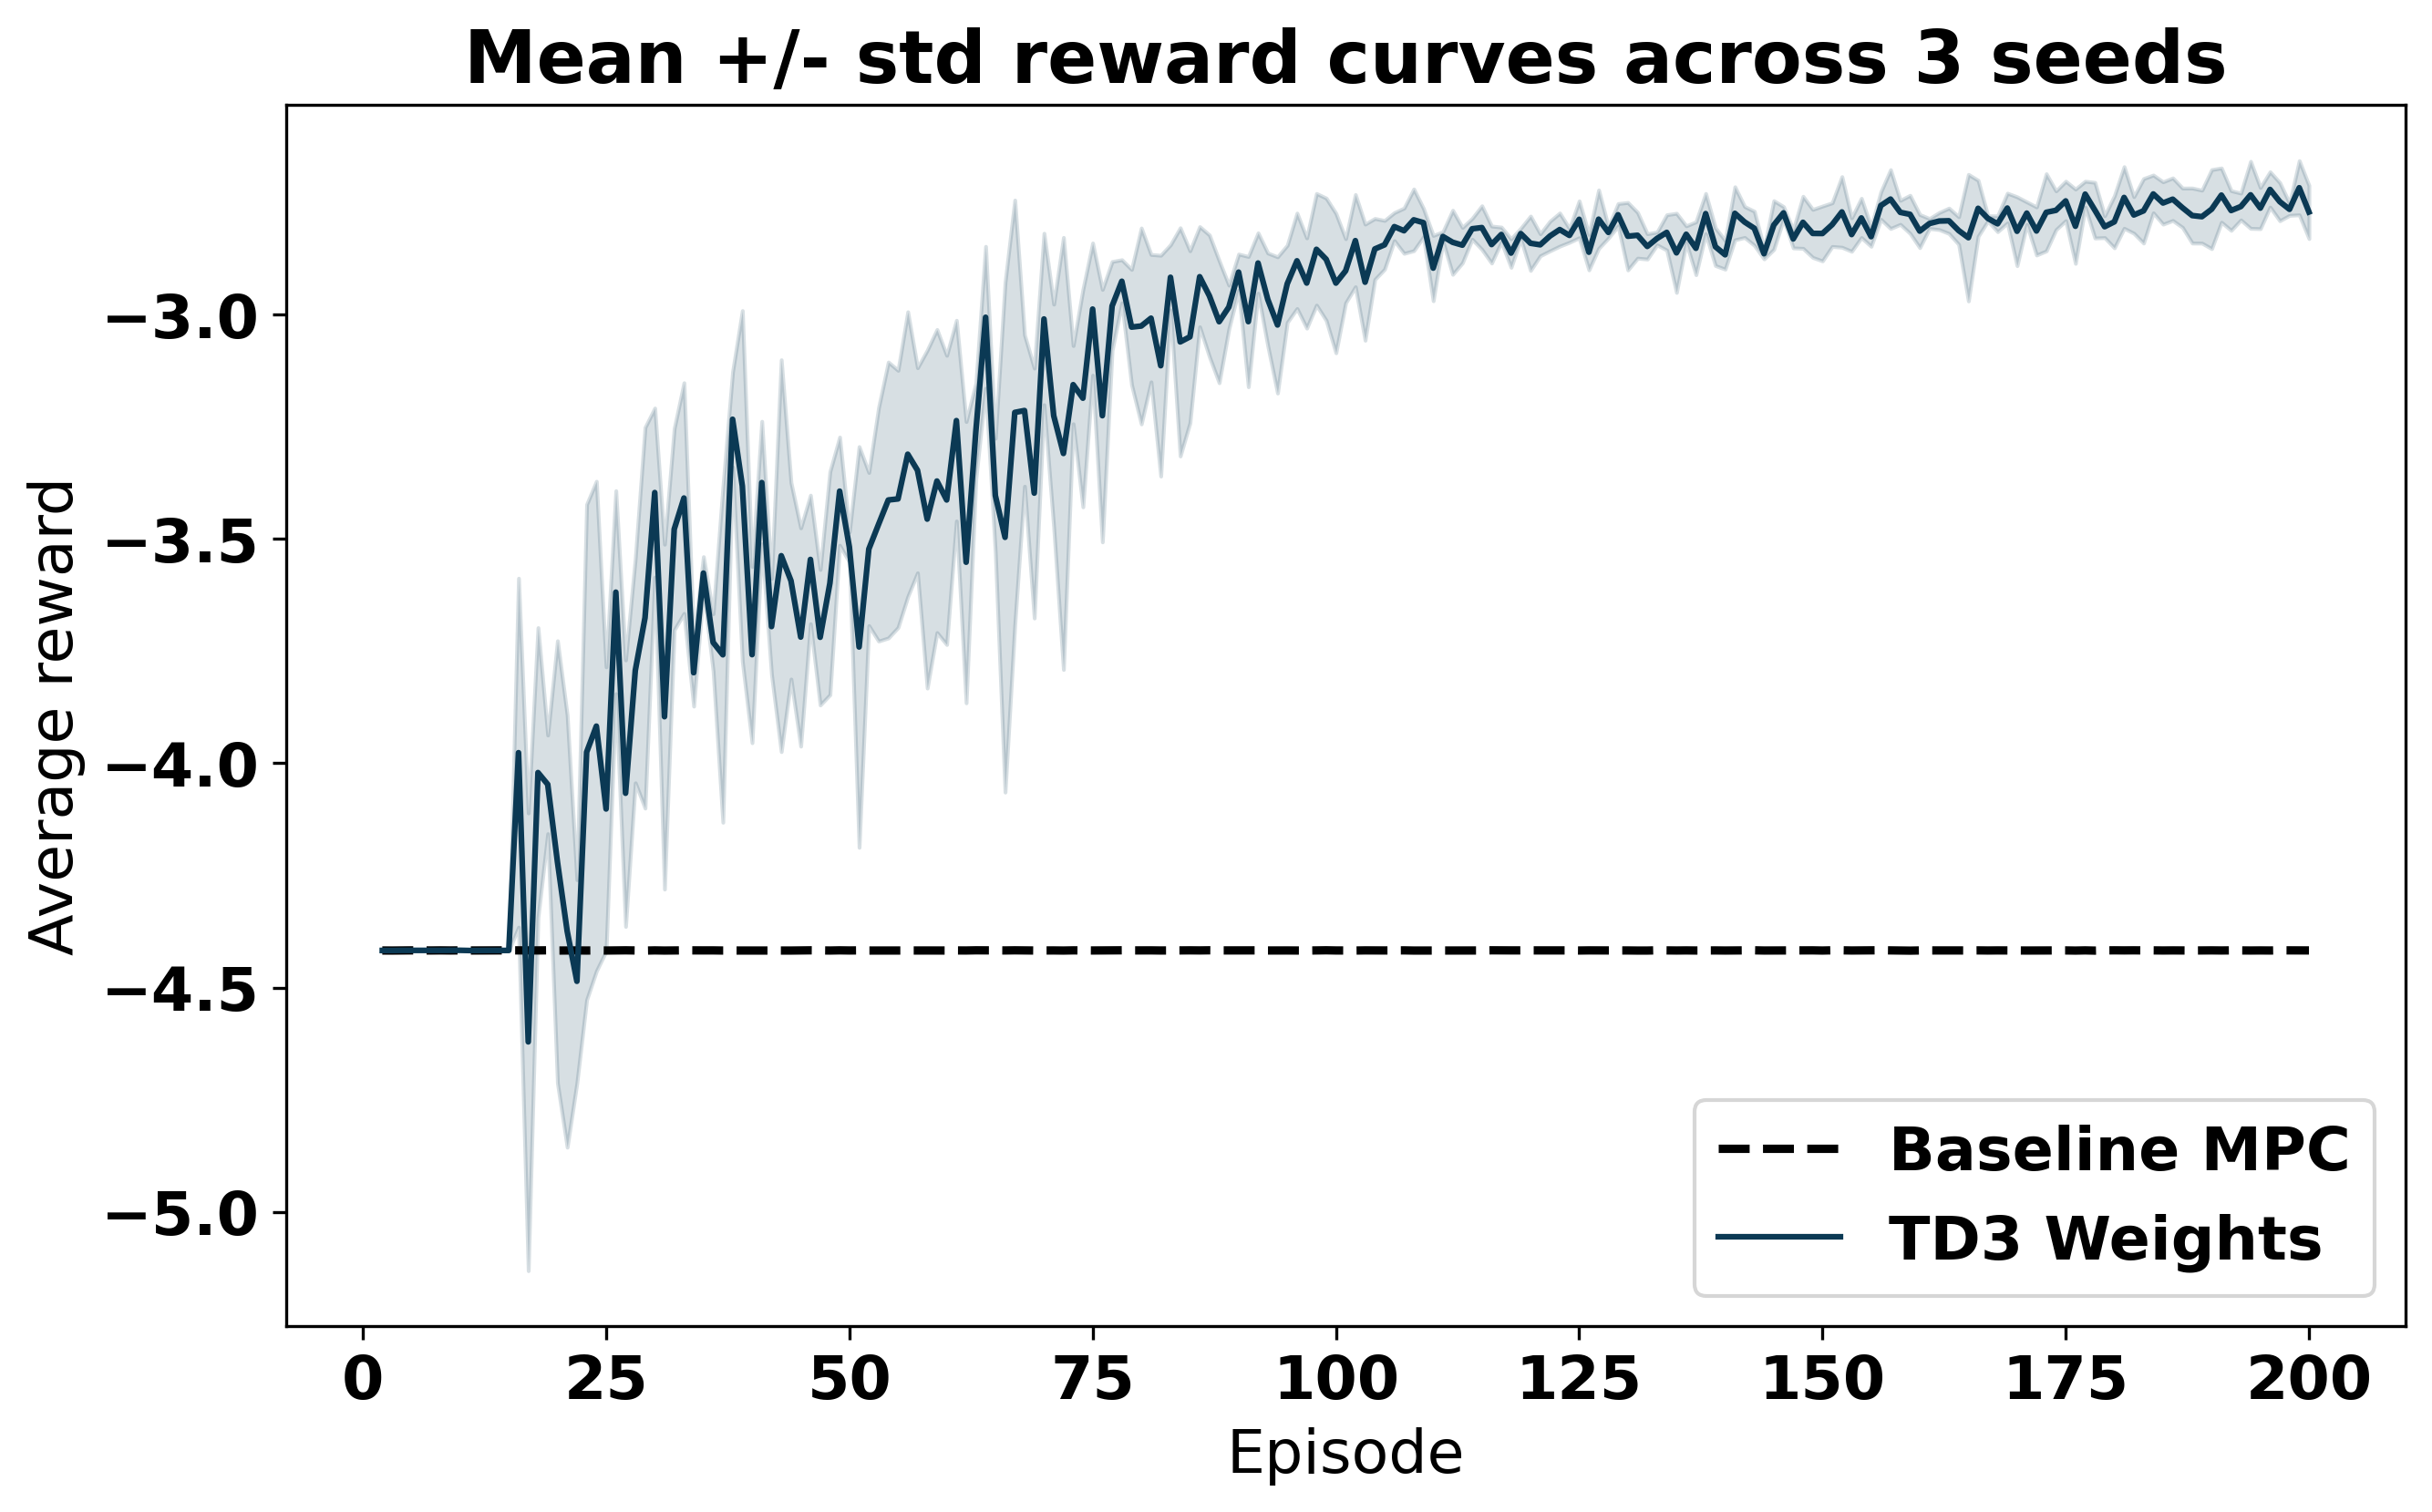
\includegraphics[
  width=\linewidth,
  height=0.20\textheight,
  keepaspectratio,
  trim=10 10 10 10,
  clip
]{figures/polymer_weights_reward.png}

\vspace{0.01cm}
{\tiny \textbf{Reward across seeds:} the weight agent climbs steadily and stabilizes near the horizon agent, though with a slightly wider spread.}

\vspace{0.02cm}
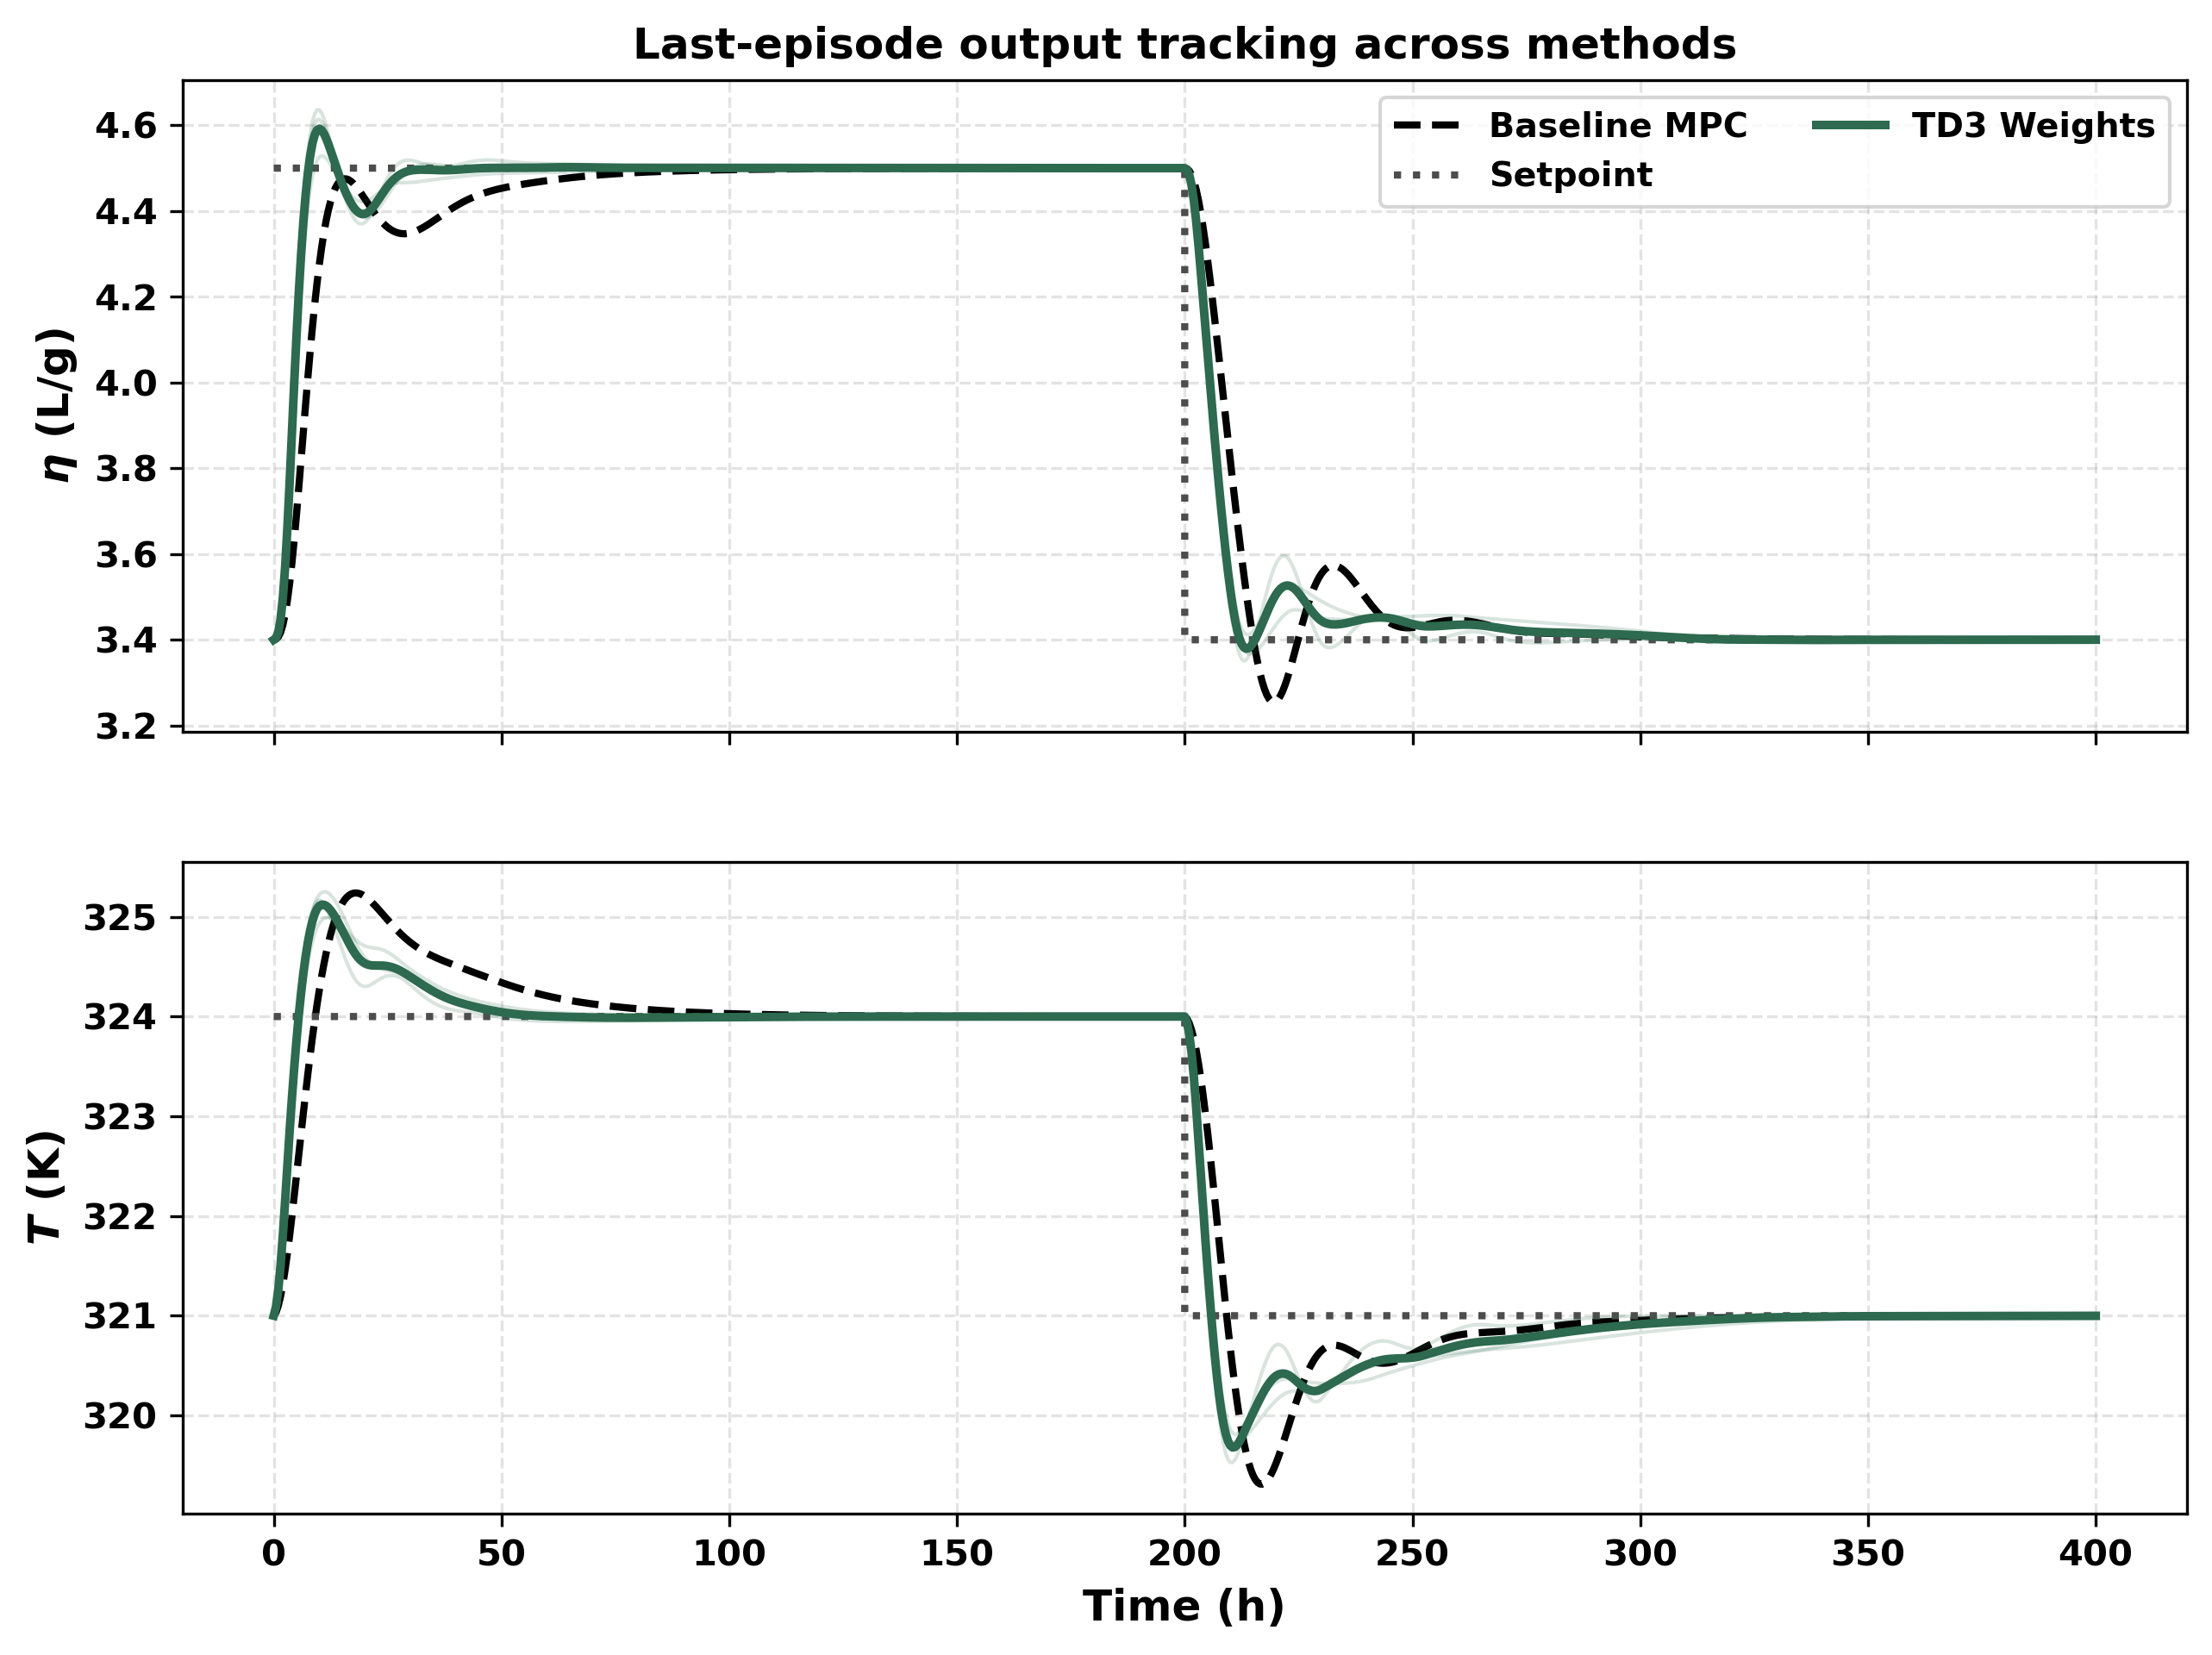
\includegraphics[
  width=\linewidth,
  height=0.31\textheight,
  keepaspectratio,
  trim=10 10 10 10,
  clip
]{figures/polymer_weights_last_episode.png}

\vspace{0.01cm}
{\tiny \textbf{Last-episode evaluation:} output tracking improves against baseline MPC while keeping the response smoother than aggressive model adaptation.}
\end{column}

\end{columns}

\takeawaybox{Online weight retuning is currently the best compromise between improvement, smooth behavior, and interpretability.}

\end{frame}

%============================= Slide 21 ============================
\begin{frame}
\setbeamertemplate{blocks}[default]
\setbeamercolor{block body}{fg=black,bg=lightgray}
\frametitle{\large \textbf{Residual Agent: RL adds a correction around the nominal MPC move}}
\scriptsize
\vspace{-0.32cm}

\begin{columns}[T,onlytextwidth]

\begin{column}{0.39\textwidth}
\begin{block}{Method}
\justifying
The residual agent preserves nominal MPC and learns only an additive correction:
\[
u_k=u_k^{\mathrm{MPC}}+\Delta u_k^{\mathrm{res}},
\]
with \(\Delta u_k^{\mathrm{res}}=\pi_\phi(s_k)\) from TD3.
The executed move is still clipped or projected to the admissible input set before it reaches the plant.
\end{block}

\vspace{0.02cm}

\begin{block}{Interpretation}
\begin{itemize}\justifying
  \setlength{\itemsep}{0.20ex}
  \item MPC keeps the stabilizing nominal policy in the loop.
  \item RL is responsible only for local correction of mismatch or missed transient behavior.
  \item This family is attractive when we want adaptation without changing the internal optimization model.
\end{itemize}
\end{block}

\vspace{0.02cm}

\begin{block}{Latest polymer result}
\justifying
Current multiseed mean:
\[
\bar{R}_{\mathrm{final}}=-3.84\pm 0.04,\quad
\overline{\mathrm{RMSE}}=0.368\pm 0.003.
\]
The mean IAE is \(12507.0\), so the residual improvement over fixed MPC is present but modest in the current exported run.
\end{block}
\end{column}

\begin{column}{0.58\textwidth}
\centering
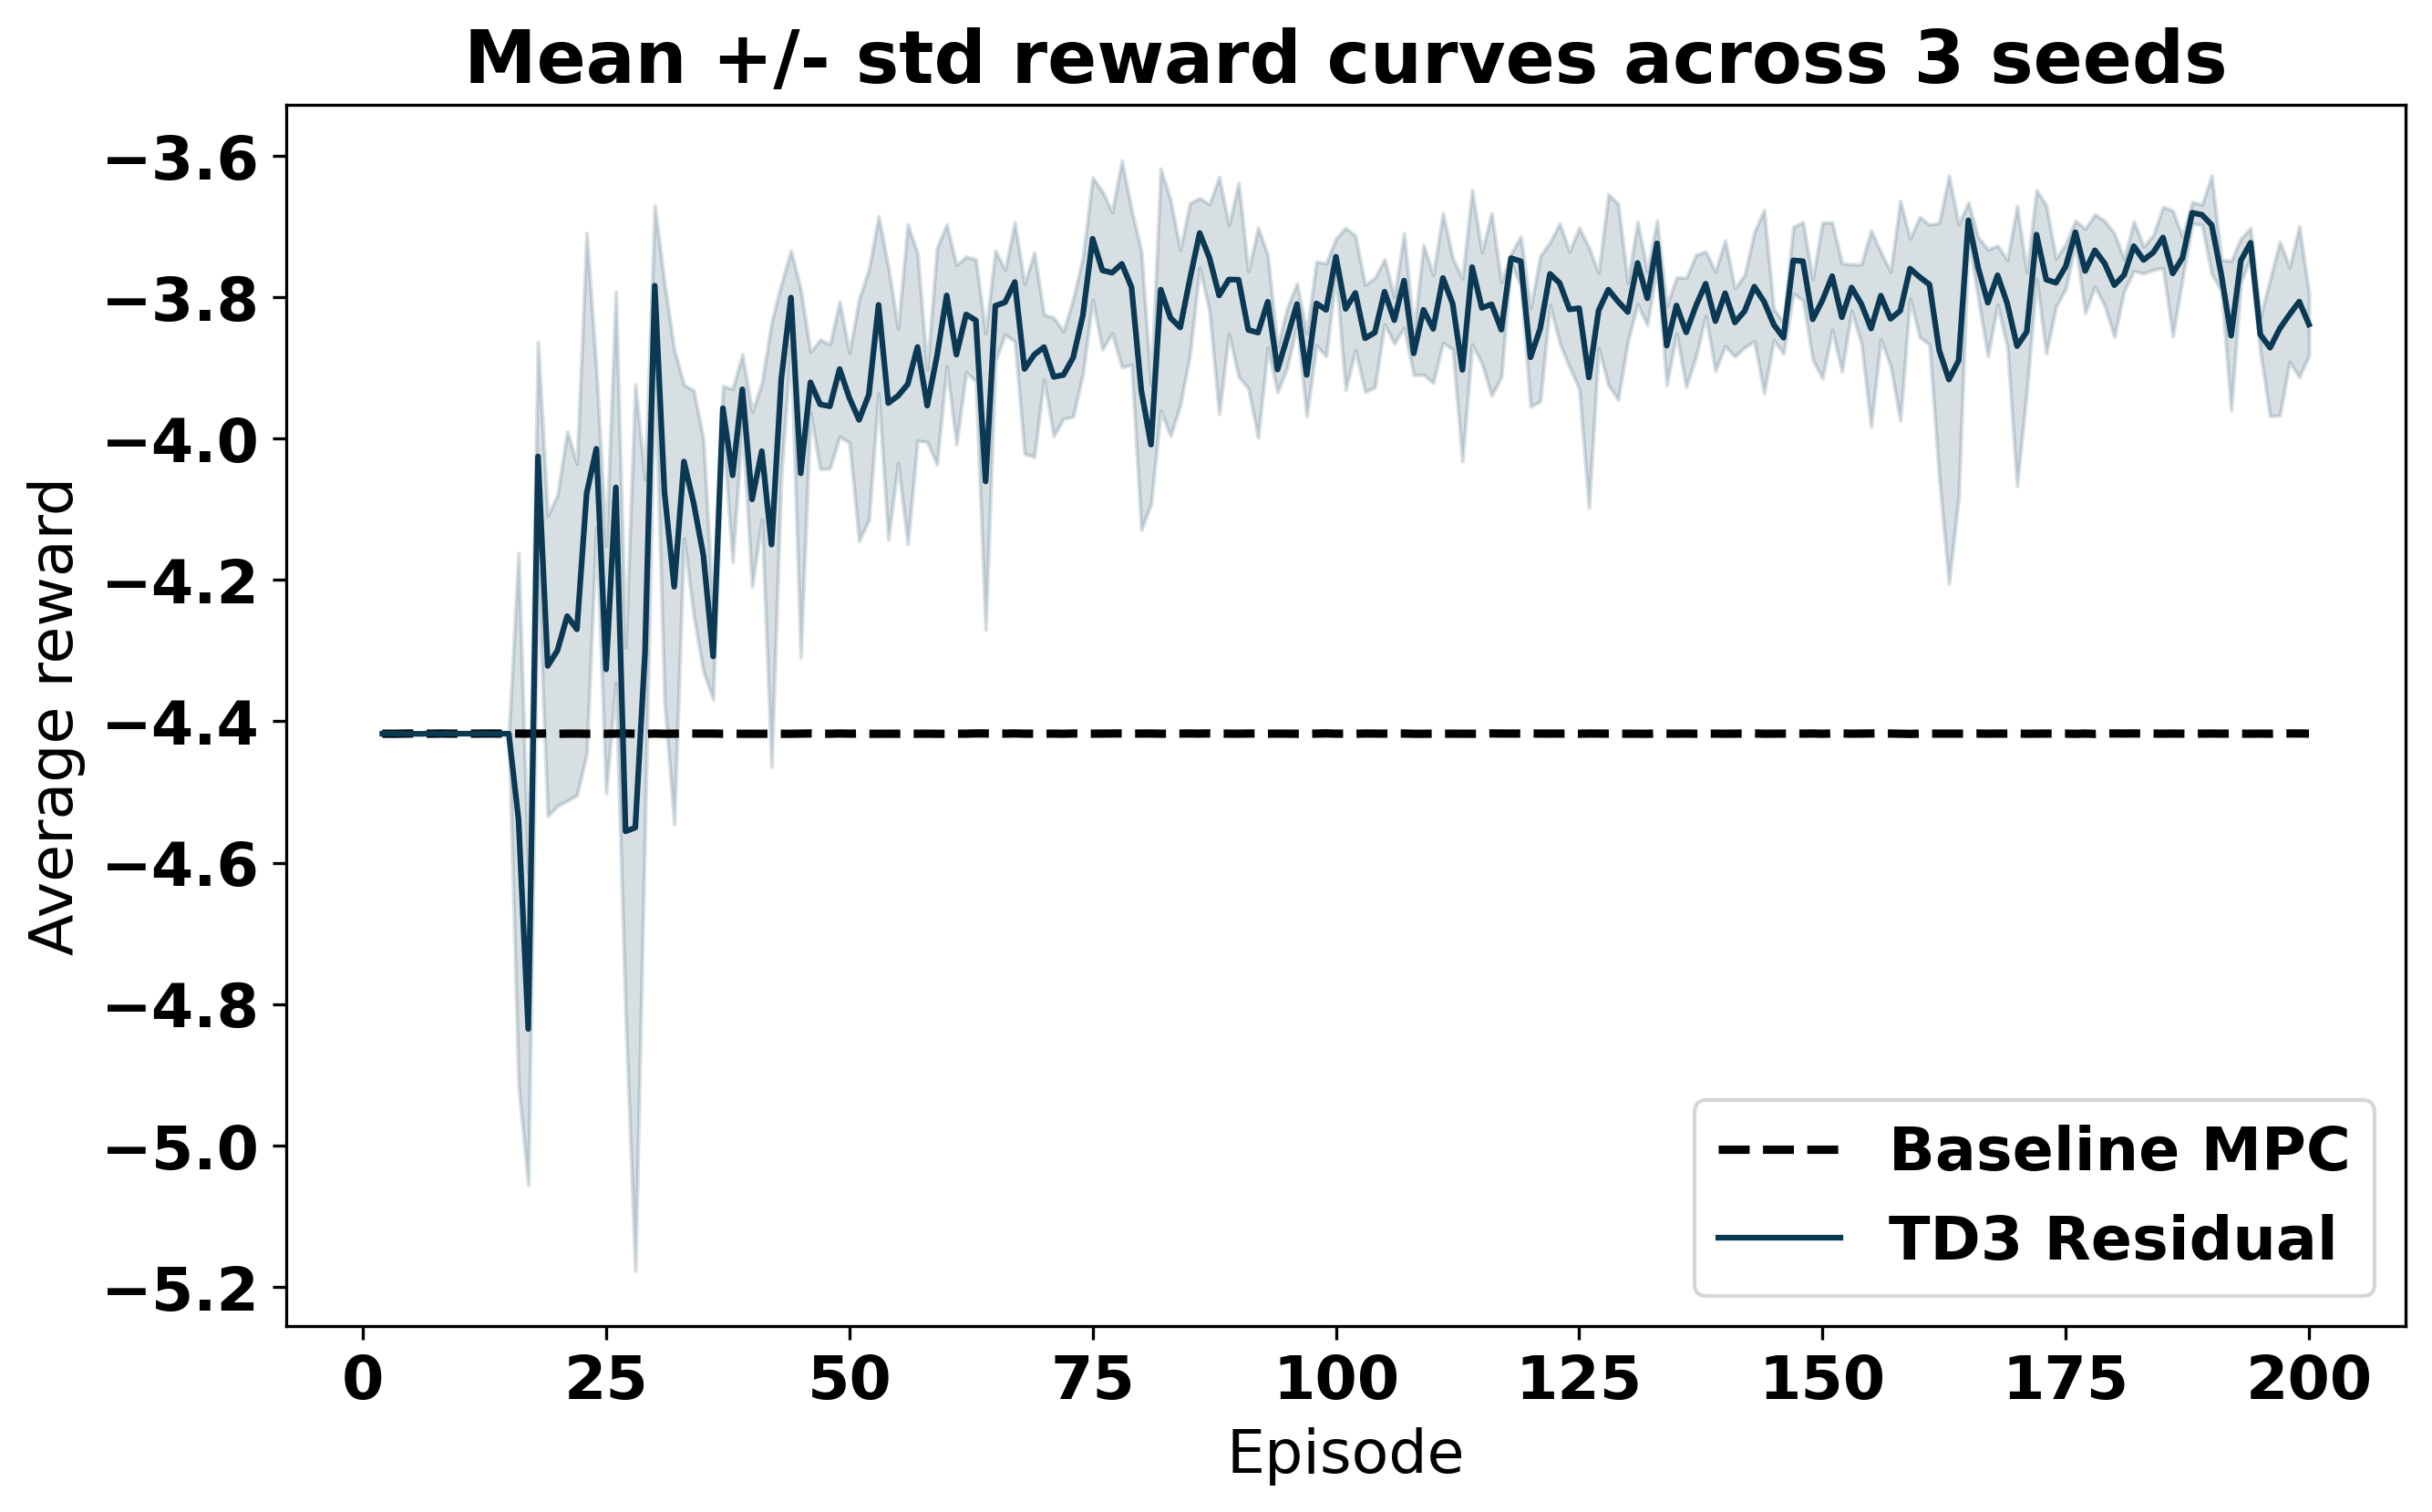
\includegraphics[
  width=\linewidth,
  height=0.20\textheight,
  keepaspectratio,
  trim=10 10 10 10,
  clip
]{figures/polymer_residual_reward.png}

\vspace{0.01cm}
{\tiny \textbf{Reward across seeds:} the residual policy improves from its initial low-reward region, but the final average remains below the horizon and weight agents.}

\vspace{0.02cm}
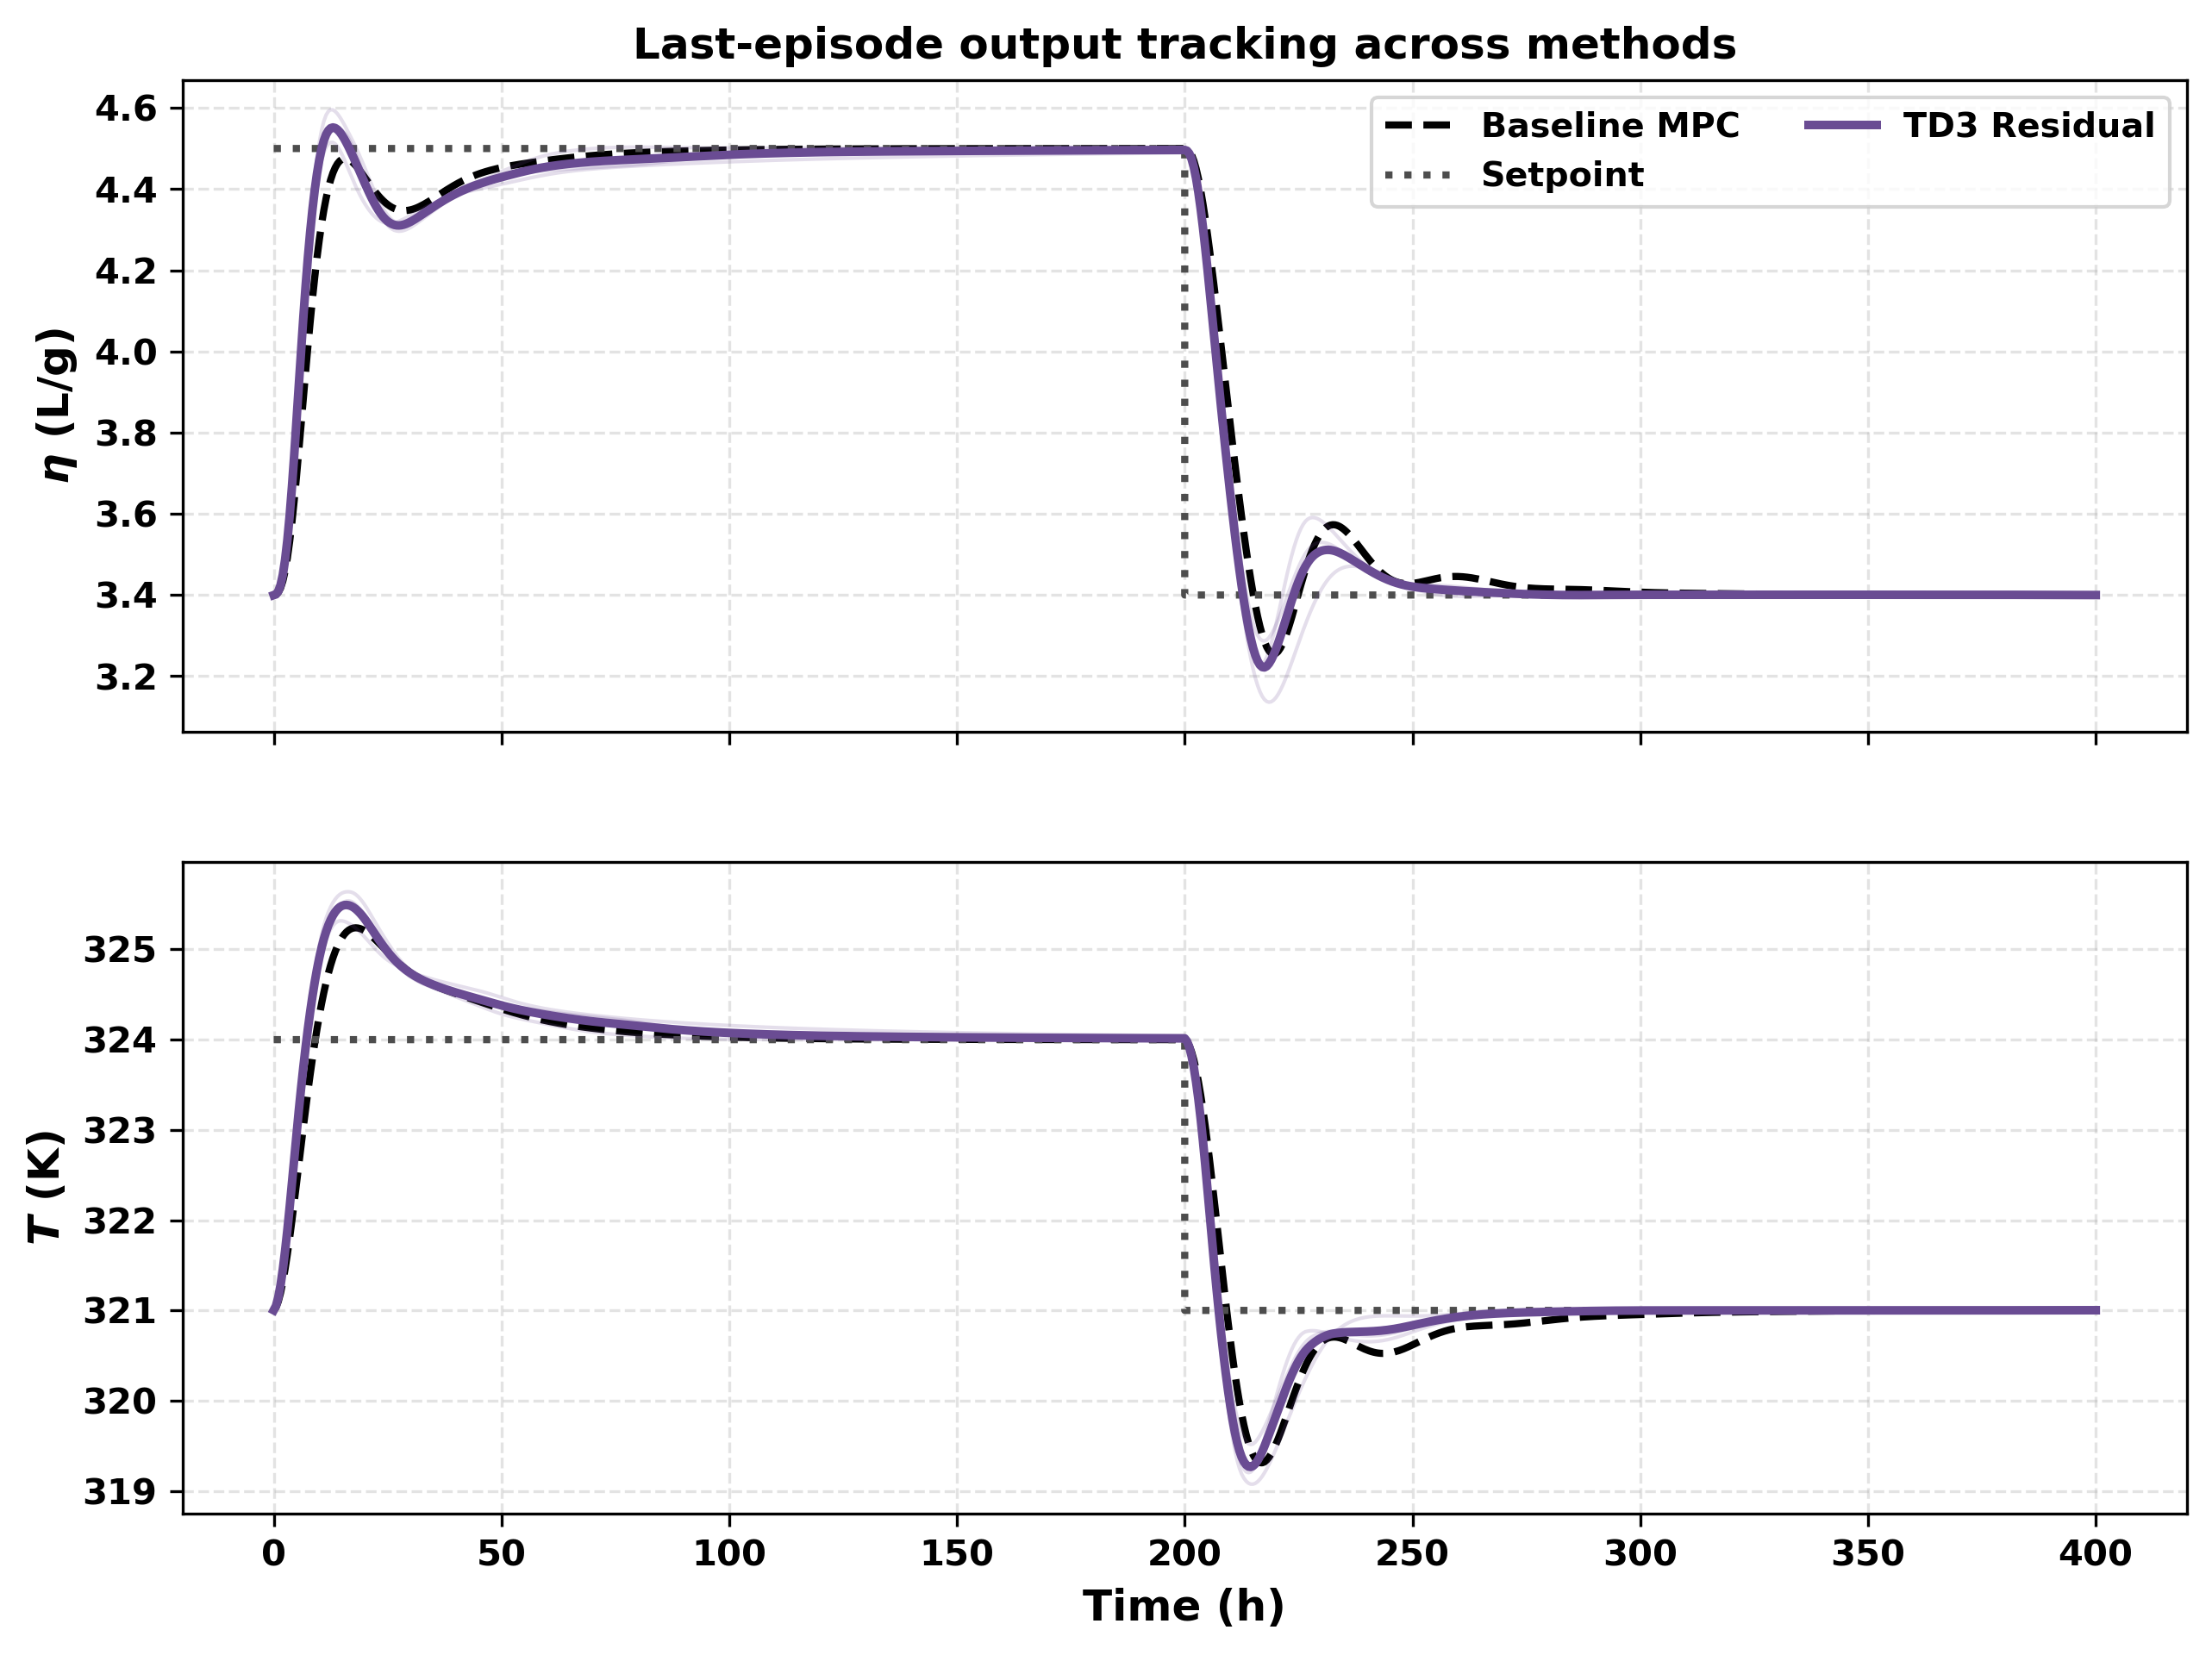
\includegraphics[
  width=\linewidth,
  height=0.31\textheight,
  keepaspectratio,
  trim=10 10 10 10,
  clip
]{figures/polymer_residual_last_episode.png}

\vspace{0.01cm}
{\tiny \textbf{Last-episode evaluation:} the residual action gives a good nominal transient, but the aggregate benefit is smaller than the best supervisory families in this notebook run.}
\end{column}

\end{columns}

\takeawaybox{Residual correction remains useful because it keeps MPC central, but its current polymer gains are weaker than adaptive horizon or adaptive weight tuning.}

\end{frame}

%============================= Slide 22 ============================
\begin{frame}
\setbeamertemplate{blocks}[default]
\setbeamercolor{block body}{fg=black,bg=lightgray}
\frametitle{\large \textbf{Project 3 keeps the direct Lyapunov target inside both MPC and RL deployment}}
\scriptsize
\vspace{-0.28cm}

\begin{columns}[T,onlytextwidth]

\begin{column}{0.47\textwidth}
\centering
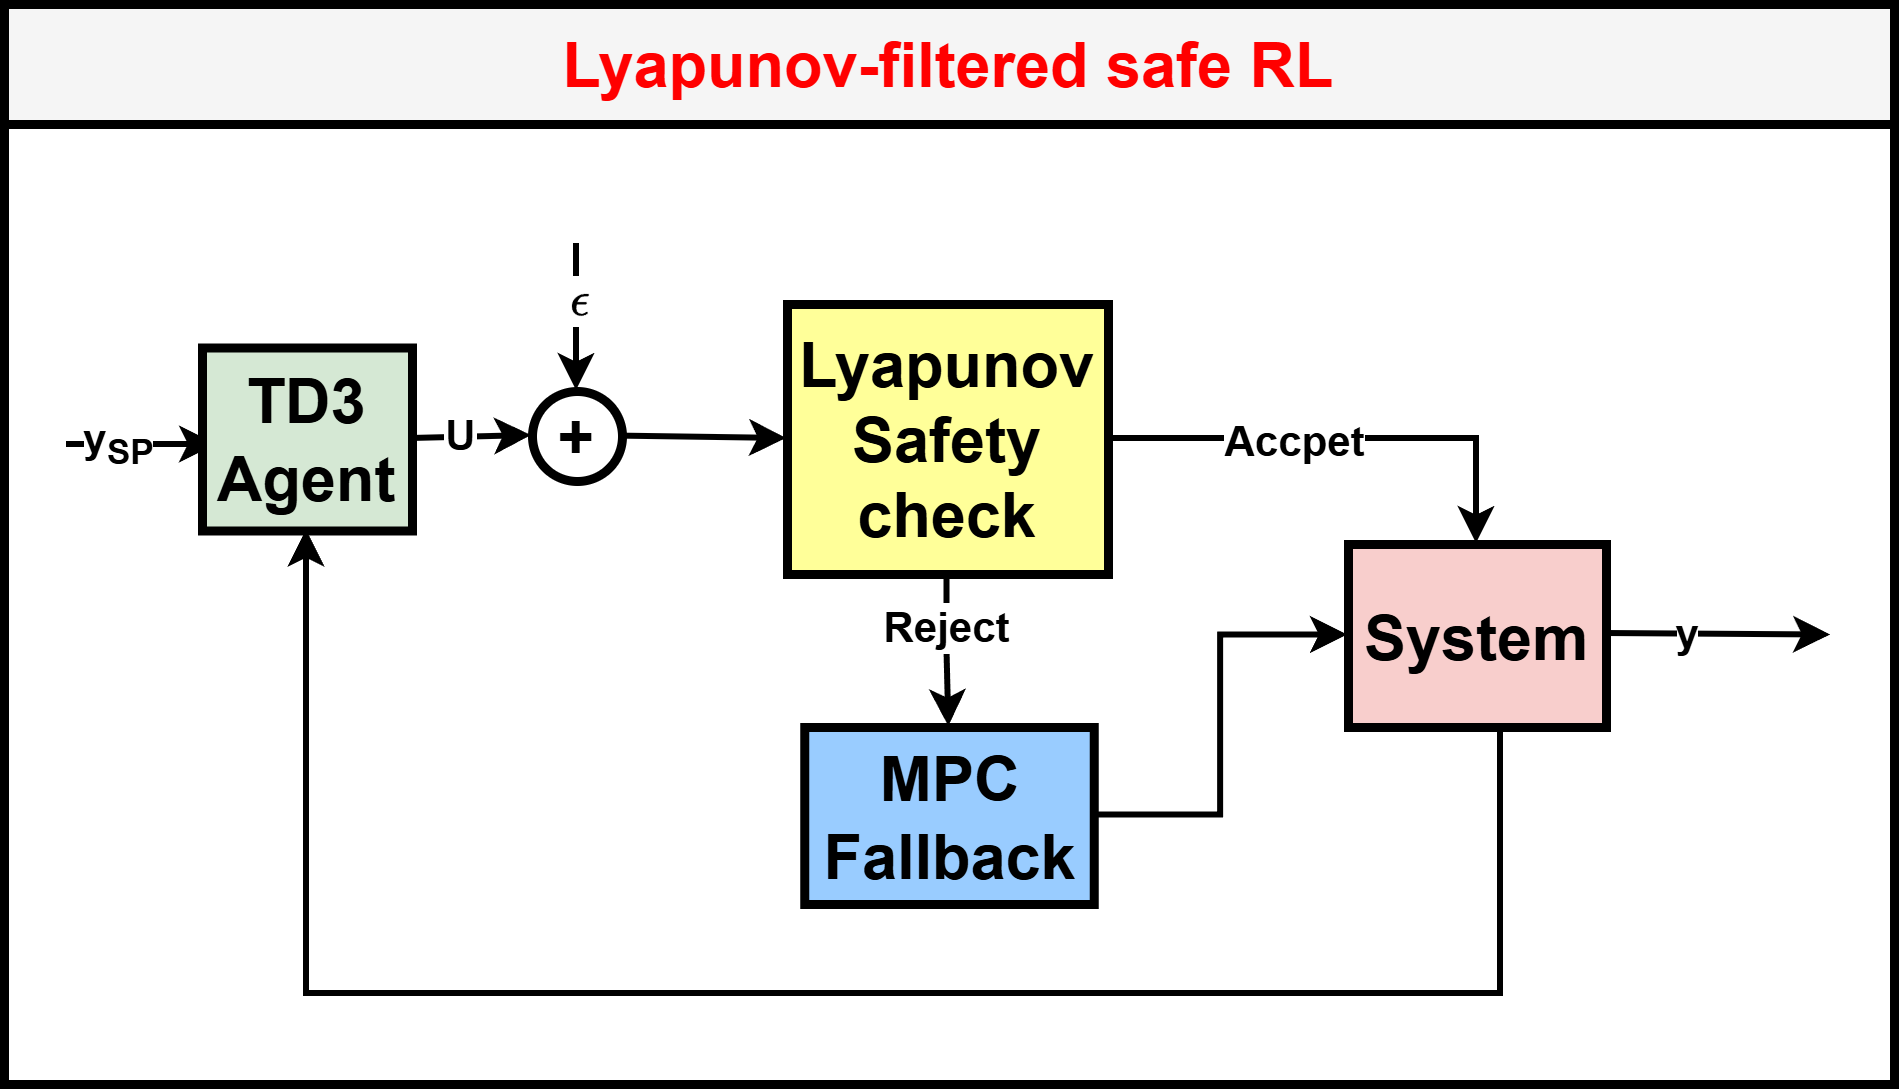
\includegraphics[
  width=\linewidth,
  height=0.58\textheight,
  keepaspectratio
]{SafeRL.png}

\vspace{0.02cm}
{\tiny \textbf{Figure:} the deployment idea is RL propose, direct Lyapunov gate certify, otherwise direct MPC fallback acts.}
\end{column}

\begin{column}{0.49\textwidth}

\begin{block}{Direct-notebook story}
\begin{itemize}\justifying
  \setlength{\itemsep}{0.28ex}
  \item The current work is centered on the direct Lyapunov notebooks, not the earlier QCQP-filter notebooks.
  \item The same hard bounded steady target is used by both the direct MPC study and the direct RL safety-gate study.
  \item The new RL entrypoints are \texttt{DirectLyapunovSafetyGateRL\_Pretrained.ipynb} and \texttt{DirectLyapunovSafetyGateRL\_ColdStart.ipynb}.
\end{itemize}
\end{block}

\vspace{0.02cm}

\begin{block}{Latest method definition}
\begin{itemize}\justifying
  \setlength{\itemsep}{0.28ex}
  \item \textbf{Target layer:} compute an admissible bounded steady target under Rawlings output-disturbance augmentation.
  \item \textbf{Direct MPC layer:} optimize tracking with a hard first-step Lyapunov contraction.
  \item \textbf{RL layer:} use a bounded TD3 action interface aligned with the practical pretrained-RL line from Project 1.
  \item \textbf{Gate:} accept the RL action only if it already satisfies the direct contraction test, otherwise solve direct Lyapunov MPC fallback.
\end{itemize}
\end{block}

\end{column}
\end{columns}

\takeawaybox{Project 3 combines the practical RL action idea with a direct Lyapunov admissible target and a model-based final authority at deployment.}

\end{frame}

%============================= Slide 23 ============================
\begin{frame}
\setbeamertemplate{blocks}[default]
\setbeamercolor{block body}{fg=black,bg=lightgray}
\frametitle{\large \textbf{Mathematics I: the hard bounded steady target is the center of the method}}
\scriptsize
\vspace{-0.30cm}

\begin{columns}[T,onlytextwidth]

\begin{column}{0.50\textwidth}
\begin{block}{Augmented model and target equations}
\justifying
The direct notebooks use Rawlings output-disturbance augmentation:
\[
x_{k+1}=Ax_k+Bu_k,\qquad d_{k+1}=d_k,\qquad y_k=Cx_k+d_k.
\]
At each step, the target stage computes
\[
(x_s,u_s,d_s,y_s)
\]
with frozen disturbance
\[
d_s=\hat d_k
\]
and bounded steady-state consistency
\[
x_s=Ax_s+Bu_s+B_d d_s,\qquad
u_{\min}\le u_s\le u_{\max}.
\]
\end{block}

\vspace{0.02cm}

\begin{block}{Bounded target variants now used}
\justifying
\[
\texttt{bounded\_hard},\qquad
\texttt{bounded\_hard\_u\_prev\_0p1},\qquad
\texttt{bounded\_hard\_xs\_prev\_0p1}.
\]
They differ only in how the bounded least-squares target is regularized:
\[
\lambda_u\|u_s-u_{k-1}\|^2
\quad \text{or} \quad
\lambda_x\|x_s-x_{s,\mathrm{prev}}\|^2.
\]
\end{block}
\end{column}

\begin{column}{0.47\textwidth}
\begin{block}{Why the target matters}
\begin{itemize}\justifying
  \setlength{\itemsep}{0.28ex}
  \item The direct controller does not track the raw setpoint by inventing an unconstrained steady center.
  \item It first chooses an admissible target that respects the model and the input box.
  \item The anchor terms are not cosmetic. They pick a consistent member of the bounded target family and suppress target drift.
\end{itemize}
\end{block}

\vspace{0.02cm}

\begin{block}{Why there are multiple bounded variants}
\begin{itemize}\justifying
  \setlength{\itemsep}{0.28ex}
  \item \texttt{bounded\_hard} is the plain formulation and serves as the baseline direct target.
  \item \texttt{bounded\_hard\_u\_prev\_0p1} adds continuity in the steady input target.
  \item \texttt{bounded\_hard\_xs\_prev\_0p1} adds continuity in the Lyapunov center itself.
\end{itemize}
\end{block}
\end{column}

\end{columns}

\takeawaybox{The key modeling choice is not only Lyapunov contraction. It is selecting a bounded steady target that stays consistent with the current operating region.}

\end{frame}

%============================= Slide 24 ============================
\begin{frame}
\setbeamertemplate{blocks}[default]
\setbeamercolor{block body}{fg=black,bg=lightgray}
\frametitle{\large \textbf{Mathematics II: direct Lyapunov contraction decides what action reaches the plant}}
\scriptsize
\vspace{-0.30cm}

\begin{columns}[T,onlytextwidth]

\begin{column}{0.52\textwidth}
\begin{block}{Direct MPC formulation}
\justifying
The online direct MPC tracks the scheduled setpoint with move suppression:
\[
\min_{\{u_{k+i|k}\}}
\sum_{i=1}^{N_p}\|y_{k+i|k}-y_{sp}\|_{Q_y}^2
+
\sum_{i=0}^{N_c-1}\|\Delta u_{k+i|k}\|_{R_{\Delta u}}^2
\]
subject to the model, bounds, and the hard first-step Lyapunov condition
\[
V_{k+1|k}^{(1)} \le \rho_{\mathrm{lyap}}V_k+\varepsilon_{\mathrm{lyap}},
\qquad
V_k=(\hat x_k-x_s)^\top P_x(\hat x_k-x_s).
\]
The latest direct reports emphasize hard bounded runs with
\[
\rho_{\mathrm{lyap}}\in\{0.98,0.985,0.99\}.
\]
\end{block}

\vspace{0.02cm}

\begin{block}{Direct RL safety gate}
\justifying
For the RL notebook, the candidate action is
\[
u_k^{RL}=\pi_\theta(s_k).
\]
If \(u_k^{RL}\) already satisfies the same direct contraction test, apply it. Otherwise solve the direct Lyapunov MPC fallback around the same \((x_s,u_s)\). If the direct target or fallback solve fails, the notebook keeps the direct semantics and holds the previous input.
\end{block}
\end{column}

\begin{column}{0.44\textwidth}
\begin{block}{Why this is the practical-stability story}
\begin{itemize}\justifying
  \setlength{\itemsep}{0.28ex}
  \item Stability is enforced at deployment through the plant-side acceptance test, not left to reward shaping alone.
  \item The pretrained notebook uses only already-available OF-MPC style data to initialize the RL action path before online learning.
  \item Replay stores the executed action, so the critic learns from what the plant actually received.
\end{itemize}
\end{block}

\vspace{0.02cm}

\begin{block}{Notebook mapping}
\begin{itemize}\justifying
  \setlength{\itemsep}{0.28ex}
  \item \texttt{DirectLyapunovMPC\_FourMethodDisturbance.ipynb} studies the direct target family on the polymer benchmark.
  \item \texttt{DirectLyapunovSafetyGateRL\_Pretrained.ipynb} is the practical deployment notebook because it starts from available data.
  \item \texttt{DirectLyapunovSafetyGateRL\_ColdStart.ipynb} is the contrast case that shows what happens without that initialization.
\end{itemize}
\end{block}
\end{column}

\end{columns}

\takeawaybox{Project 3 aims for practical stability by certifying or replacing each RL move with the same direct Lyapunov target structure used by the direct MPC controller.}

\end{frame}

%============================= Slide 25 ============================
\begin{frame}
\setbeamertemplate{blocks}[default]
\setbeamercolor{block body}{fg=black,bg=lightgray}
\frametitle{\large \textbf{Mathematics III: RL with a direct Lyapunov acceptance gate}}
\tiny
\vspace{-0.30cm}

\begin{columns}[T,onlytextwidth]

\begin{column}{0.54\textwidth}
\begin{block}{State, action, target, and gate}
\justifying
\[
s_k=\big[\hat x_k^{aug},\, y_k^{sp},\, u_{k-1}\big].
\]
\[
a_k=\pi_\theta(s_k),\qquad u_k^{RL}=\mathcal{M}(a_k),
\]
\[
(x_{s,k},u_{s,k},d_{s,k},y_{s,k})=\mathcal{T}(\hat x_k^{aug},y_k^{sp},u_{k-1}).
\]
\[
e_k^x=\hat x_k-x_{s,k},\qquad
V_k=(e_k^x)^\top P_x e_k^x .
\]
\[
\hat x_{k+1|k}^{RL}=A\hat x_k+B u_k^{RL}+B_d d_{s,k},
\]
\[
e_{k+1|k}^{RL}=\hat x_{k+1|k}^{RL}-x_{s,k},
\qquad
V_{k+1|k}^{RL}=(e_{k+1|k}^{RL})^\top P_x e_{k+1|k}^{RL},
\]
\[
V_{k+1|k}^{RL}\le \rho_{\mathrm{lyap}}V_k+\varepsilon_{\mathrm{lyap}}.
\]
\end{block}

\vspace{0.02cm}

\begin{block}{Applied action and replay tuple}
\justifying
\[
u_k^{exec}=
\begin{cases}
u_k^{RL}, & \text{if } V_{k+1|k}^{RL}\le \rho_{\mathrm{lyap}}V_k+\varepsilon_{\mathrm{lyap}},\\
u_k^{LMPC}, & \text{otherwise},
\end{cases}
\]
\[
\tau_k=(s_k,\; a_k^{exec},\; r_k,\; s_{k+1},\; 0),\qquad
a_k^{exec}=\mathcal{M}^{-1}(u_k^{exec}).
\]
\[
s_{k+1}=\big[\hat x_{k+1}^{aug},\, y_k^{sp},\, u_k^{exec}\big].
\]
\end{block}
\end{column}

\begin{column}{0.42\textwidth}
\begin{block}{Reward and replay are intentionally unchanged}
\justifying
\[
r_k=r_{\mathrm{Proj2}}(e_k,\Delta u_k,y_k^{sp}),
\]
\[
e_k=y_k-y_k^{sp},\qquad
\Delta u_k=u_k^{exec}-u_{k-1},\qquad
\mathcal{B}_{k+1}=\mathcal{B}_k\cup\{\tau_k\}.
\]
\end{block}

\vspace{0.02cm}

\begin{block}{Replay-buffer and TD3 update}
\justifying
For a batch \((s_i,a_i,r_i,s_i')\sim\mathcal{B}\),
\[
y_i=r_i+\gamma \min_{j=1,2}Q_{\phi_j^-}\!\left(s_i',\pi_{\theta^-}(s_i')+\epsilon_i\right).
\]
\[
\nabla_\theta J \approx \frac{1}{N}\sum_i \nabla_a Q_{\phi_1}(s_i,a)\vert_{a=\pi_\theta(s_i)}\nabla_\theta \pi_\theta(s_i).
\]
\[
\theta,\phi \leftarrow \mathrm{TD3Train}(\mathcal{B}),\qquad
s_k \rightarrow a_k \rightarrow \mathcal{T} \rightarrow \text{check} \rightarrow u_k^{exec} \rightarrow \tau_k \rightarrow \mathcal{B}.
\]
\end{block}

\vspace{0.02cm}

\begin{block}{Key distinction}
\justifying
Project 3 adds a target-and-Lyapunov gate before the plant, while keeping the Project 2 reward and replay logic.
\end{block}
\end{column}

\end{columns}

\takeawaybox{Project 3 reuses the same Project 2 reward and replay pipeline, but inserts a mathematically explicit target-and-Lyapunov gate between the actor output and the plant.}

\end{frame}

%============================= Slide 26 ============================
\begin{frame}
\setbeamertemplate{blocks}[default]
\setbeamercolor{block body}{fg=black,bg=lightgray}
\frametitle{\large \textbf{Project 3 closes the loop between practical RL initialization and direct Lyapunov deployment}}
\scriptsize
\vspace{-0.28cm}

\begin{columns}[T,onlytextwidth]

\begin{column}{0.56\textwidth}
\begin{block}{Scientific message}
\begin{itemize}\justifying
  \setlength{\itemsep}{0.30ex}
  \item Project 1 showed that pretraining is the practical way to avoid unsafe random online RL initialization.
  \item Project 3 carries that idea into a direct Lyapunov notebook family where every applied move is checked against the admissible target.
  \item The method is therefore built around what is available in practice: an existing OF-MPC policy, plant-side constraints, and limited closed-loop data.
\end{itemize}
\end{block}

\vspace{0.02cm}

\begin{block}{Deployment logic}
\begin{itemize}\justifying
  \setlength{\itemsep}{0.30ex}
  \item Build a bounded steady target that is model-consistent and operationally meaningful.
  \item Use that same target inside either the direct MPC controller or the pretrained RL safety gate.
  \item Apply the RL move only when the direct Lyapunov condition is already satisfied, otherwise revert to the direct controller logic.
\end{itemize}
\end{block}
\end{column}

\begin{column}{0.38\textwidth}
\begin{block}{Current status for the talk}
\begin{itemize}\justifying
  \setlength{\itemsep}{0.30ex}
  \item The direct Lyapunov notebooks now give a clean mathematical definition for Project 3.
  \item This section is intentionally method-only and stops at deployment logic.
  \item Polymer and Aspen Dynamics \(C_2\) studies remain outside this slide sequence.
\end{itemize}
\end{block}

\vspace{0.02cm}

\begin{block}{One-sentence close}
\justifying
Project 1 makes RL practical, Project 2 makes MPC adaptive, and Project 3 adds a direct Lyapunov target-and-gate layer so the final move is bounded, interpretable, and stability-oriented before it reaches the plant.
\end{block}
\end{column}

\end{columns}

\takeawaybox{The Project 3 message is methodological: use available data to initialize learning, then use the direct Lyapunov target-and-gate structure to control what finally reaches the plant.}

\end{frame}

\end{document}
